\documentclass[letterpaper,11pt]{article}

\usepackage[utf8]{inputenc}
\usepackage[spanish]{babel}
\usepackage[
    letterpaper,
    top=1.7cm,
    bottom=2cm,
    left=2cm,
    right=2cm
]{geometry}

\usepackage{graphicx}
\usepackage{fancyhdr}
\usepackage[table,xcdraw]{xcolor}
\usepackage{tikz}
\usetikzlibrary{shapes.geometric, shapes.symbols, arrows, positioning, fit, backgrounds, calc, babel, decorations.pathreplacing}
\usepackage{ifpdf}
\usepackage[cmex10]{amsmath}
\usepackage{amssymb}
\usepackage{amsfonts}
\usepackage{float}
\usepackage{siunitx}
\usepackage{listings}
\usepackage{hyperref}
\usepackage{booktabs}
\usepackage{url}
\usepackage{titlesec}
\usepackage[export]{adjustbox}
\usepackage{parskip}
\usepackage[numbers]{natbib}
\usepackage{ragged2e}
\usepackage{array}
\usepackage{longtable}
\usepackage{multirow}
\usepackage{pgfplots}
\pgfplotsset{compat=1.17}
\usepackage{makecell}
\usepackage{caption}
\usepackage{subcaption}

\newcolumntype{L}[1]{>{\RaggedRight\arraybackslash}p{#1}}

\hypersetup{colorlinks=false,bookmarksopen=true,linkbordercolor={1 1 1}}
\newcommand{\rfigura}[1]{Fig.\,\ref{#1}}
\newcommand{\rtabla}[1]{Tabla \ref{#1}}

\newcommand{\Curso}{IEE2913 --- Diseño Eléctrico (Capstone)}
\newcommand{\TituloInforme}{Informe de Avance 3 (60\,\%)}
\newcommand{\NumeroGrupo}{10}
\newcommand{\NombreProyecto}{SupaClock}
\newcommand{\Integrantes}{Tomás Avendaño, Benjamín Sepúlveda, Pablo Uribe}
\newcommand{\FechaEntrega}{1 de junio de 2026}

\graphicspath{{./}{../Entrega2/}{../../mechanical/}{../../hardware/SupaClock_Carrier/}}

\lstset{
  basicstyle=\ttfamily\small,
  breaklines=true,
  breakatwhitespace=true,
  postbreak=\mbox{\textcolor{red}{$\hookrightarrow$}\space},
  captionpos=b,
  frame=single,
  numbers=left,
  numberstyle=\tiny\color{gray},
  language=C,
  keywordstyle=\color{blue}\bfseries,
  commentstyle=\color{gray}\itshape,
  stringstyle=\color{red!70!black},
  showstringspaces=false,
  inputencoding=utf8,
  extendedchars=true,
  literate=
    {á}{{\'a}}1 {é}{{\'e}}1 {í}{{\'i}}1 {ó}{{\'o}}1 {ú}{{\'u}}1
    {Á}{{\'A}}1 {É}{{\'E}}1 {Í}{{\'I}}1 {Ó}{{\'O}}1 {Ú}{{\'U}}1
    {ñ}{{\~n}}1 {Ñ}{{\~N}}1 {ü}{{\"u}}1 {Ü}{{\"U}}1
    {¿}{{?`}}1 {¡}{{!`}}1 {°}{{$^\circ$}}1
}

\begin{document}

% =========== Encabezado ===========
\noindent
\begin{minipage}[c]{0.12\textwidth}
    
\includegraphics[width=0.9\linewidth]{logo.pdf}
\end{minipage}
\hfill
\begin{minipage}[c]{0.68\textwidth}
    \small
    PONTIFICIA UNIVERSIDAD CATÓLICA DE CHILE\\
    ESCUELA DE INGENIERÍA\\
    Departamento de Ingeniería Eléctrica\\
    \Curso
\end{minipage}
\hfill
\begin{minipage}[c]{0.15\textwidth}
    \raggedleft
    \small
    Grupo \NumeroGrupo
\end{minipage}

\vspace{0.4cm}

\begin{center}
    {\Large \textbf{\TituloInforme}}\\[0.4cm]
\end{center}

\noindent\textbf{Proyecto:} \NombreProyecto\\
\textbf{Integrantes:} \Integrantes\\
\textbf{Fecha:} \FechaEntrega

\hrule

\vspace{0.5cm}

\renewcommand{\contentsname}{Índice}
\tableofcontents
\listoffigures
\listoftables
\newpage

% =====================================================
\section*{Resumen}
\addcontentsline{toc}{section}{Resumen}
% =====================================================

Este informe consolida el trabajo desarrollado entre el 4 de mayo de 2026 y el 1 de junio de 2026 para el proyecto \textbf{\NombreProyecto}, un dispositivo biométrico diseñado para el monitoreo continuo de actividad física, frecuencia cardíaca, oxigenación, temperatura, electrocardiografía y detección de caídas. 

El eje de esta entrega es la \textbf{transición a la unidad integrada}. Mientras que la fase anterior validó el funcionamiento de los subsistemas aislados (como el firmware multitarea, la telemetría BLE y el procesamiento local de ECG), esta etapa consolida la plataforma física y digital final: el microcontrolador \textbf{Seeed XIAO ESP32-S3} montado sobre una \textbf{PCB carrier} de diseño propio, alojada en una \textbf{carcasa de protección impresa}, una \textbf{aplicación móvil Flutter} que actúa como interfaz y un procesador de \textbf{Machine Learning (CNN 1D)} para clasificar la actividad física y detectar caídas en tiempo real.

Los entregables producidos durante esta iteración son:
\begin{itemize}
    \item \textbf{Firmware para el microcontrolador ESP32-S3} con soporte para PSRAM, depuración por puerto USB nativo, administración de energía dinámica con modo de bajo consumo y una arquitectura modular estructurada en la biblioteca \texttt{supaclock\_app}.
    \item \textbf{Algoritmo de pasos por FFT} acelerado por hardware para sustituir el detector temporal previo. Se incluye un entorno de pruebas que verifica la precisión, el rechazo de falsos positivos y el filtro de histéresis.
    \item \textbf{PCB Carrier}: placa integradora de dos caras compatible con los procesos de fabricación por fresado del FabLab, diseñada y validada eléctricamente.
    \item \textbf{Carcasa protectora}: envolvente ergonómico de dos piezas atornilladas que integra soportes para la correa, botones mecánicos y aberturas alineadas para los sensores ópticos y térmicos.
    \item \textbf{Aplicación móvil Flutter} con interfaz dual (de usuario y de desarrollo), análisis Pan-Tompkins local, base de datos persistente y almacenamiento en la nube de señales de alta frecuencia.
    \item \textbf{Machine Learning (CNN 1D)}: modelo de tres capas entrenado con datos de movimiento del propio sensor para la clasificación de actividad física, alocado en PSRAM y ejecutado de manera asíncrona.
    \item \textbf{Interfaz gráfica rediseñada} con paletas de color configurables, fuentes legibles de alta resolución y almacenamiento de gráficos optimizado en PSRAM para liberar memoria interna.
\end{itemize}

El avance del proyecto alcanza un 65\,\% ponderado. El diseño del carrier y el modelado de la carcasa están terminados, el firmware sobre S3 está portado, la clasificación por Machine Learning tiene sus algoritmos base operativos y la app móvil cuenta con sus funciones esenciales. Tras fabricar y ensamblar físicamente la PCB con éxito en el FabLab, los componentes e interfaces están operativos. Las actividades finales se concentrarán ahora en corregir detalles mecánicos (footprint de botones, sujeción de pantalla) y realizar la validación final de la unidad cerrada.

\newpage

% =====================================================
\section{Introducción}
% =====================================================

El presente informe se organiza en torno a los tres ejes definidos para esta etapa: el diagrama de bloques, la planificación actualizada y la implementación con sus resultados experimentales. Cada sección detalla los fundamentos de diseño y las pruebas de validación correspondientes. Los listados de código y tablas de soporte se incluyen en los anexos para agilizar la lectura del documento.

Para el estado de los bloques se mantiene la codificación cromática previa: verde para subsistemas validados, amarillo para implementaciones parciales y rojo punteado para tareas pendientes. La nomenclatura de archivos y entornos de desarrollo corresponde al repositorio Git del proyecto.

\subsection{Contexto del periodo y avances logrados}

Al término de la fase anterior, el sistema contaba con las siguientes bases:
\begin{itemize}
    \item Firmware multitarea sobre ESP32-C3 con soporte para sensores inerciales, de temperatura, de pulso óptico y acondicionamiento analógico de electrocardiografía (ECG).
    \item Pan-Tompkins \cite{pan_tompkins} en Python validado en diferido sobre capturas de señal real, con el código fuente disponible en el repositorio.
    \item Telemetría BLE para la transmisión de variables y señales continuas a través de servicios personalizados de baja latencia.
    \item Administración de energía dinámica con DFS y modo de bajo consumo activo.
    \item Modos de funcionamiento configurables por el usuario y persistidos en memoria interna.
\end{itemize}

Durante este periodo, el desarrollo se concentró en los siguientes hitos de integración:
\begin{itemize}
    \item \textbf{Migración del firmware al Seeed XIAO ESP32-S3} con soporte para PSRAM y depuración por puerto USB nativo.
    \item \textbf{Rediseño del PCB} mediante el desarrollo de la placa de integración compatible con el equipamiento de fabricación del FabLab.
    \item \textbf{Nueva carcasa protectora} de dos piezas con esquinas redondeadas, ranuras de sujeción para correa estándar y botones mecánicos integrados.
    \item \textbf{Algoritmo de pasos por FFT} acelerado por hardware para sustituir el detector temporal previo. Se incluye un entorno de pruebas que verifica la precisión, el rechazo de falsos positivos y el filtro de histéresis.
    \item \textbf{Machine Learning (CNN 1D)}: modelo de clasificación de actividad física entrenado e integrado bajo el entorno de ejecución en PSRAM.
    \item \textbf{Aplicación móvil Flutter} que gestiona la telemetría BLE, realiza el análisis de ECG localmente y almacena los datos de forma persistente.
    \item \textbf{Refactorización del firmware} hacia una arquitectura modular en la biblioteca \texttt{supaclock\_app}.
    \item \textbf{Rediseño de la interfaz gráfica} con temas dinámicos y optimización en la memoria de pantalla.
\end{itemize}

El resto del informe profundiza en cada uno de estos avances desde la perspectiva de hardware, firmware y validación experimental.

\newpage

% =====================================================
\section{Diagrama de bloques de bajo nivel}
% =====================================================

\subsection{Estado vigente}

El diagrama de alto nivel de la entrega 1 (siete dominios: interacción, energía, sensores, MCU, interfaz local, \textit{gateway}, \textit{backend}) se mantiene estructuralmente sin cambios. Lo que sí evolucionó respecto al diagrama de bloques de bajo nivel presentado en la entrega 2 es lo siguiente:
\begin{enumerate}
    \item \textbf{El bloque MCU pasa a XIAO ESP32-S3} \cite{esp32s3_ds_2024}, lo que simplifica la sección de potencia y reconfigura la asignación de pines.
    \item \textbf{El bloque ``PCB SuperMini''} desaparece y se reemplaza por el \textbf{``PCB Carrier v1''}, que es el integrador físico de la unidad.
    \item \textbf{El bloque ``Machine Learning (CNN 1D)''} transita de \textit{pendiente} (rojo punteado) a \textit{parcial} (amarillo, 80\,\% de implementación) gracias al entrenamiento sobre datos de sensores propios y la integración en el firmware.
\end{enumerate}

La \rfigura{fig:lownivel_e3} reproduce el diagrama de bajo nivel vigente. Su contenido refleja el estado de cada subsistema al 1 de junio de 2026.

\begin{figure}[H]
    \centering
    \resizebox{\textwidth}{!}{\begin{tikzpicture}[
    node distance=0.6cm and 0.9cm,
    every node/.style={font=\scriptsize},
    blockOK/.style={rectangle, rounded corners, draw=black!70, very thick, fill=green!22, text width=2.8cm, align=center, minimum height=0.95cm},
    blockPart/.style={rectangle, rounded corners, draw=black!70, very thick, fill=yellow!28, text width=2.8cm, align=center, minimum height=0.95cm},
    blockTodo/.style={rectangle, rounded corners, draw=black!70, very thick, dashed, fill=red!12, text width=2.8cm, align=center, minimum height=0.95cm},
    energy/.style={rectangle, rounded corners, draw=black!70, very thick, fill=orange!22, text width=2.6cm, align=center, minimum height=0.9cm},
    mcu/.style={rectangle, rounded corners, draw=black, very thick, fill=blue!22, text width=3.4cm, align=center, minimum height=1.4cm, font=\small\bfseries},
    busI2C/.style={->, >=stealth, thick, blue!70!black},
    busSPI/.style={->, >=stealth, thick, violet!80!black},
    adc/.style={->, >=stealth, thick, orange!85!black},
    gpio/.style={->, >=stealth, thick, teal!70!black},
    ble/.style={->, >=stealth, thick, dashed, blue!60},
    pwr/.style={->, >=stealth, thick, red!70},
    legend/.style={rectangle, draw=black!50, fill=white, inner sep=4pt}
]
% ============== MCU (Centro) ==============
\node[mcu] (mcu) {XIAO ESP32-S3\\FreeRTOS + LVGL 8.4\\\textbf{Funcionando}};

% ============== INTERFAZ LOCAL (Izquierda) ==============
\node[blockOK, left=2.2cm of mcu] (st7789) {ST7789 1.69" IPS\\\textbf{100\%} (LVGL)};
\node[blockOK, above=0.3cm of st7789] (btns) {2 botones GPIO\\\textbf{100\%} (debounce)};
\node[blockOK, below=0.3cm of st7789] (gui) {GUI: Home/Bio/Menu\\\textbf{100\%} (7 pant.)};

% ============== ENERGÍA (Arriba a la Izquierda) ==============
\node[energy, left=0.6cm of st7789] (sgm40567) {Cargador SGM40567\\\textbf{100\%} (XIAO S3)};
\node[energy, above=0.3cm of sgm40567] (sgm6029) {Buck SGM6029 3.3\,V\\\textbf{100\%} (XIAO S3)};
\node[blockOK, above=0.3cm of sgm6029] (fuel) {MAX17048\\\textbf{100\%} (I2C)};

\node[energy, left=0.6cm of sgm40567] (usbc) {USB-C\\\textbf{100\%} (XIAO S3)};
\node[energy, above=0.3cm of usbc] (bms) {BMS TP4056+DW01A\\\textbf{100\%} (Carrier)};
\node[energy, above=0.3cm of bms] (lipo) {Bater\'ia LiPo 3.7\,V\\\textbf{100\%} (502030)};

% ============== SENSORES I2C y ADC (Derecha) ==============
\node[blockOK, right=2.2cm of mcu, yshift=1.8cm] (max205) {MAX30205\\\textbf{100\%} \textit{(0x48)}};
\node[blockOK, below=0.3cm of max205] (bmi) {BMI160 IMU\\\textbf{100\%} \textit{(0x68)}};
\node[blockOK, below=0.3cm of bmi] (max102) {MAX30102\\\textbf{95\%} HR/SpO\textsubscript{2}};
\node[blockOK, below=0.3cm of max102] (ad8232) {AD8232 + DMA\\\textbf{100\%} \textit{(GPIO1)}};

% ============== ECOSISTEMA (Abajo) ==============
\node[blockOK, below=1.8cm of mcu] (ble) {BLE NimBLE\\\textbf{100\%} (3 GATT chr.)};
\node[blockOK, right=0.8cm of ble] (cli) {Cliente PC testing\\\textbf{100\%} (\texttt{logger})};
\node[blockOK, right=0.8cm of cli] (fb) {Firebase (Cloud Fn)\\\textbf{100\%} (Pan-Tomp.)};

\node[blockOK, below=0.6cm of ble] (app) {App m\'ovil (gateway)\\\textbf{90\%} (Flutter)};
\node[blockOK, right=0.8cm of app] (pcb) {PCB Carrier v1\\\textbf{100\%} (Listo)};
\node[blockPart, right=0.8cm of pcb] (ml) {TinyML (CNN 1D)\\\textbf{70\%} (Falta capt. datos)};

% ============== Conexiones de Potencia ==============
\draw[pwr] (usbc) -- (bms);
\draw[pwr] (lipo) -- (bms);
\draw[pwr] (lipo) -- (fuel);
\draw[pwr] (bms)  -- (sgm6029);
\draw[pwr] (usbc) -- (sgm40567);
\draw[pwr] (sgm40567) -- (sgm6029);
\draw[pwr] (sgm6029.west) -- ++(-0.2,0) |- ([yshift=0.4cm]fuel.north) -| ([xshift=-1.2cm]mcu.north);

% ============== Conexiones I2C ==============
\draw[busI2C] (fuel.east) -| ([xshift=-0.6cm]mcu.north);

% Enrutamiento ortogonal tipo "bus" para alinear sensores de la derecha
\draw[busI2C] (max205.west) -- ++(-0.6,0) |- node[right, pos=0.25, font=\tiny]{I2C 400\,kHz} ([yshift=0.5cm]mcu.east);
\draw[busI2C] (bmi.west)    -- ++(-0.6,0) |- ([yshift=0.15cm]mcu.east);
\draw[busI2C] (max102.west) -- ++(-0.6,0) |- ([yshift=-0.2cm]mcu.east);

% ============== Conexiones ADC ==============
\draw[adc] (ad8232.west) -- ++(-0.6,0) |- node[below, pos=0.75, font=\tiny]{ADC1 20\,kHz} ([yshift=-0.55cm]mcu.east);

% ============== Conexiones SPI/GPIO ==============
\draw[busSPI] (mcu.west) -- node[above]{SPI 80\,MHz} (st7789.east);
\draw[gpio] (btns.east) -- ++(0.4,0) |- node[above, pos=0.8, font=\tiny]{GPIO} ([yshift=0.4cm]mcu.west);

% ============== Conexiones Ecosistema ==============
\draw[ble] (mcu) -- (ble);
\draw[ble] (ble) -- node[above, font=\tiny, align=center]{GATT\\3 chr.} (cli);
\draw[gpio, ->] (cli) -- node[above]{Wi-Fi} (fb);
\draw[ble, ->] (ble) -- (app);
\draw[ble, ->] (app.south) -- ++(0,-0.4) -| (fb.south);

% ============== Leyenda ==============
\node[legend, below=1.2cm of pcb] (leg) {%
\begin{tabular}{ll}
\textcolor{green!50!black}{$\blacksquare$} Listo &
\textcolor{red!70}{\textbf{$\rightarrow$}} Potencia \\
\textcolor{yellow!60!black}{$\blacksquare$} Parcial &
\textcolor{blue!70!black}{$\rightarrow$} I2C 400\,kHz \\
\textcolor{red!70!black}{$\blacksquare$} Pendiente &
\textcolor{violet!80!black}{$\rightarrow$} SPI 80\,MHz \\
\textcolor{blue!60}{$\dashrightarrow$} BLE/Wi-Fi &
\textcolor{orange!85!black}{$\rightarrow$} ADC/DMA \\
\end{tabular}};
\end{tikzpicture}
}
    \caption{Diagrama de bloques de bajo nivel al cierre del avance 3. El MCU central (XIAO ESP32-S3) integra los buses I$^2$C (BMI160, MAX30102, MAX30205, MAX17048), SPI (ST7789), ADC con DMA (AD8232) y GPIO (botones, backlight). La sección de potencia muestra la cadena de alimentación y monitoreo por el MAX17048. El ecosistema cierra el flujo de telemetría y procesamiento mediante la aplicación móvil y algoritmos locales.}
    \label{fig:lownivel_e3}
\end{figure}

\subsection{Cambios respecto al diagrama de la entrega anterior}

\subsubsection{MCU: del ESP32-C3 al XIAO ESP32-S3}

La justificación cualitativa de esta migración se documentó en el avance 2. En esta entrega la migración se materializó, y los cambios concretos en el diagrama son:
\begin{itemize}
    \item \textbf{Procesamiento y memoria.} El XIAO ESP32-S3 cuenta con un procesador dual-core a 240\,MHz y soporte de memoria PSRAM. Esto permite alojar la interfaz gráfica y la ejecución de Machine Learning en memoria externa, liberando la SRAM interna y distribuyendo las tareas de manera asíncrona.
    \item \textbf{Mapa de pines reasignado.} Aunque el chip cuenta con múltiples líneas de entrada y salida, solo una cantidad limitada de pines son accesibles físicamente en el formato DIP/THT del módulo. Esto redujo los pines disponibles para el prototipo, forzando a economizar conexiones y a implementar el reset del ST7789 por software para liberar un GPIO físico.
    \item \textbf{Sección de potencia simplificada.} El cargador y regulador auxiliar TP4056 externo del carrier v1 fue puenteado; en su lugar, se utilizó el BMS interno del microcontrolador Seeed S3, soldando los cables de la batería LiPo directamente a los dos pines SMD inferiores del módulo.
    \item \textbf{Aceleración por hardware.} Se integraron las librerías del fabricante para aprovechar las instrucciones de cálculo vectorial del procesador en el algoritmo de pasos y en la inferencia de Machine Learning.
\end{itemize}

\subsubsection{PCB: del esquemático del módulo al Carrier v1}

Se descartó el esquemático de prueba preliminar y se desarrolló una placa integradora de dos caras compatible con los procesos de fresado del FabLab. El diseño optimiza el uso del espacio físico y eléctrico. El carrier emplea un sistema de zócalos (sockets) para prácticamente todos los componentes y breakout boards, lo que facilita el desmontaje, mantenimiento o reemplazo de los sensores y de la Seeed S3 sin comprometer las soldaduras principales de la placa.

\subsubsection{Machine Learning: de pendiente a parcial}

El modelo de Machine Learning (CNN 1D) se integró en el firmware como biblioteca interna. El estado del bloque es parcial por dos razones:
\begin{enumerate}
    \item \textbf{Datos empíricos de caídas}: La clase de caídas se valida inicialmente con datos simulados y modelados físicamente, quedando la toma de registros empíricos reales para la etapa de pruebas integradas de la unidad.
    \item \textbf{Validación física}: La inferencia continua está operativa, y su comportamiento final se evaluará con la unidad totalmente ensamblada y bajo movimiento libre.
\end{enumerate}

\subsubsection{Otros cambios menores en el diagrama}

\begin{itemize}
    \item \textbf{Rediseño de interfaz gráfica}: Se agregaron temas visuales dinámicos y fuentes tipográficas optimizadas para mejorar la visualización en pantalla, gestionando los gráficos desde la PSRAM.
    \item \textbf{Aplicación móvil}: La app de Flutter reemplaza al monitor de pruebas en PC y asume la telemetría BLE y el almacenamiento local persistente de variables clínicas.
    \item \textbf{Procesamiento local de ECG}: Se reubicó el algoritmo Pan-Tompkins directamente en el cliente móvil para priorizar una arquitectura de \textit{edge computing}, dejando la nube únicamente como compendio de datos e histórico para el usuario.
    \item \textbf{Cliente PC}: Se conserva el cliente de pruebas en PC como alternativa de depuración para tareas específicas de bajo nivel.
\end{itemize}

\subsection{Especificaciones detalladas por bloque}

La \rtabla{tab:specs_e3} consolida las especificaciones cuantitativas vigentes al cierre del avance 3.

\begin{longtable}{|L{2.6cm}|L{2.0cm}|L{2.6cm}|L{4.6cm}|L{2.0cm}|}
\caption{Especificaciones de bajo nivel por bloque y estado de implementación.} \label{tab:specs_e3} \\
\hline
\rowcolor{gray!20}\textbf{Bloque} & \textbf{Interfaz} & \textbf{Tasa / frecuencia} & \textbf{Especificación clave} & \textbf{Estado} \\ \hline
\endfirsthead
\multicolumn{5}{c}{\tablename\ \thetable{} -- continuación de la página anterior} \\
\hline
\rowcolor{gray!20}\textbf{Bloque} & \textbf{Interfaz} & \textbf{Tasa / frecuencia} & \textbf{Especificación clave} & \textbf{Estado} \\ \hline
\endhead
\hline
\endfoot
XIAO ESP32-S3 & --- & 240\,MHz dual-core & SRAM interna + PSRAM + Flash; USB nativo; cargador y regulador integrados & \cellcolor{green!20}100\,\% \\ \hline
AD8232 (ECG) & ADC1 / DMA & 20\,kHz $\to$ 500\,Hz & GPIO1 ADC, ganancia analógica 1100, down-sample por software & \cellcolor{green!20}100\,\% \\ \hline
BMI160 (IMU) & I$^2$C, 0x68 & 100\,Hz polling (modelo a 50\,Hz) & Rango configurable, FIFO interna; polling vía task de movimiento & \cellcolor{green!20}100\,\% \\ \hline
MAX30102 (PPG) & I$^2$C, 0x57 & 100 sps efectivos & Emisión RED+IR, filtro digital y promediado de muestras en el sensor & \cellcolor{green!20}95\,\% \\ \hline
MAX30205 (Temp) & I$^2$C, 0x48 & 1/30--1/900\,Hz (por modo) & Conversión de alta resolución con precisión clínica & \cellcolor{green!20}100\,\% \\ \hline
MAX17048 (Fuel) & I$^2$C, 0x36 & 1/30\,Hz & Monitoreo del estado de carga y voltaje por algoritmo interno & \cellcolor{green!20}100\,\% \\ \hline
ST7789 (Display) & SPI & 60 FPS & Controlador de pantalla gráfica, DMA activo, reset por software & \cellcolor{green!20}100\,\% \\ \hline
Botones & GPIO polling & 30\,Hz & Monitoreo de botones físicos con filtrado de rebotes por software & \cellcolor{green!20}100\,\% \\ \hline
BMS Seeed S3 & Integrado & --- & Carga LiPo conectada directamente a los pines SMD del microcontrolador & \cellcolor{green!20}100\,\% \\ \hline
BLE NimBLE & 2,4\,GHz BLE & Periódico & Conexión y transmisión inalámbrica de telemetría de bajo consumo & \cellcolor{green!20}100\,\% \\ \hline
GUI LVGL & Gráfica & 60 FPS & Pantallas de interfaz gráfica con temas y fuentes optimizadas en PSRAM & \cellcolor{green!20}100\,\% \\ \hline
Power Management & esp\_pm & Dinámico & Bajo consumo activo mediante modos de suspensión del procesador & \cellcolor{green!20}100\,\% \\ \hline
Power Modes & NVS & --- & Configuración de perfiles de energía persistentes en memoria interna & \cellcolor{green!20}100\,\% \\ \hline
\textbf{PCB Carrier} & 2 capas & --- & Placa de integración de dos caras fabricada y validada en el FabLab & \cellcolor{green!20}\textbf{100\,\% ensamblado} \\ \hline
\textbf{Carcasa} & Plástico impreso & --- & Envolvente ergonómico de dos piezas impreso y validado mecánicamente & \cellcolor{green!20}\textbf{100\,\% impreso} \\ \hline
\textbf{Machine Learning} & CNN 1D & 0.5\,Hz inferencia & Clasificación de actividad física probada de forma offline mediante red convolucional & \cellcolor{yellow!25}\textbf{80\,\%} \\ \hline
\textbf{Podómetro} & Análisis FFT & Periódico & Conteo de pasos en frecuencia con filtro de ruido e histéresis & \cellcolor{green!20}\textbf{100\,\%} \\ \hline
\textbf{App Flutter} & BLE + Nube & --- & Interfaz dual de telemetría, análisis de ECG local y sincronización & \cellcolor{green!20}\textbf{90\,\%} \\ \hline
Pan-Tompkins & Dart local & En cliente & Algoritmo de detección de picos QRS para cálculo de frecuencia y HRV & \cellcolor{green!20}100\,\% \\ \hline
Servicios Cloud & Triggers & Diferido & Respaldo para almacenamiento y análisis secundario de datos en la nube & \cellcolor{yellow!25}50\,\% \\ \hline
\end{longtable}

\subsection{Justificación de los cambios en el diseño}

\subsubsection{Procesamiento ECG en cliente vs. Cloud Function}

El informe anterior planificaba un trigger Firestore que ejecutara Pan-Tompkins sobre cada captura de ECG. Durante el desarrollo de la app móvil se evaluó este flujo bajo los siguientes criterios:
\begin{itemize}
    \item \textbf{Priorización de Edge Computing.} En lugar de saturar la red y gastar poder de cómputo en la nube para procesar la señal de ECG en vivo (lo cual es innecesario), se priorizó el cálculo local directo en el dispositivo del usuario. De esta forma, la nube opera únicamente como un compendio e histórico de datos.
    \item \textbf{Autonomía y offline-first.} Mover el procesamiento al cliente convierte el reporte de HRV en una función autónoma e independiente de la conectividad de red, permitiendo que la aplicación opere incluso en modo sin conexión y reduciendo costos innecesarios en la nube.
\end{itemize}

La decisión fue mantener \texttt{firebase/functions/main.py} en el repositorio como \textit{fallback} y referencia algorítmica, pero que el camino primario para los usuarios sea \texttt{app/lib/services/pan\_tompkins.dart}. Ambos flujos ejecutan idénticos pasos de procesamiento.

\subsubsection{Algoritmo de pasos: FFT en lugar de umbral temporal}

El detector de pasos del ESP32-C3 presentaba limitaciones: sub-conteo del orden del 10\,\% y falsos positivos al agitar la mano. La migración a un análisis espectral FFT, implementado en el archivo \texttt{step\_algorithm.c} (dentro de \texttt{lib/step\_algorithm/}), resuelve esto aprovechando el target S3. El nuevo algoritmo es estructuralmente distinto:
\begin{enumerate}
    \item Acumula 128 muestras de magnitud lineal del acelerómetro a 50\,Hz ($\approx$2,56\,s de ventana física).
    \item Solo procesa si la energía rotacional es suficiente (\texttt{max\_gyro\_val $>$ 400 LSB} $\approx 25$\,°/s), eliminando vibraciones ajenas a la caminata.
    \item Remueve el sesgo DC y aplica \textbf{ventana de Hann} vía \texttt{dsps\_wind\_hann\_f32}.
    \item Calcula la \textbf{FFT radix-2 acelerada} por PIE (\texttt{dsps\_fft2r\_fc32} + \texttt{dsps\_bit\_rev\_fc32}) en 220\,$\mu$s.
    \item Busca el pico de potencia en la banda de caminata $[0,75\,\text{Hz}, 2,75\,\text{Hz}]$ y compara contra un umbral empírico $\text{UMBRAL\_FFT} = 1\cdot10^9$.
    \item Aplica \textbf{histéresis temporal de dos ventanas}: la primera detección no descarga pasos sino que los guarda en cache; solo si una segunda ventana consecutiva supera el umbral se acumulan ambos, eliminando falsos positivos por movimientos aislados.
\end{enumerate}

\subsubsection{Carcasa V2: del \textit{box} rectangular a un envelope estilizado}

La iteración v1 era un \textit{bounding box} funcional pero estéticamente plano. El rediseño V2 introduce:
\begin{itemize}
    \item \textbf{Esquinas verticales redondeadas} con $r\_vert = 12$\,mm, aproximando la huella de un reloj clásico.
    \item \textbf{Chamfer inferior y superior} de $r\_chamfer = 1,5$\,mm, suavizando las transiciones.
    \item \textbf{Taper de 2\,mm} entre la base y el techo, reduciendo el perfil de ``ladrillo'' y mejorando la ergonomía.
    \item \textbf{\textit{Lugs} tipo ``stadium''} integrados, con ancho de 20\,mm para correa estándar y contrafuertes robustos de 5\,mm.
    \item \textbf{\textit{Button caps} como piezas separadas} con \textit{flange} exterior, transmitiendo la pulsación mecánica sin debilitar la carcasa.
    \item \textbf{Dimensión final 98$\times$79$\times$25\,mm}, ajustada a la PCB carrier y con cavidades interiores para alojar la batería.
\end{itemize}

Durante las pruebas iniciales se corrigieron dos fallas: se confirmó que la orientación de la ventana del MAX30102 en el primer diseño era geométricamente correcta (descartando rotaciones adicionales), y se extendió el cutter cilíndrico de los orificios laterales a 16\,mm de profundidad para atravesar por completo las paredes curvas originadas por el taper y el chamfer.

\newpage

% =====================================================
\section{Planificación actualizada}
% =====================================================

\subsection{Contraste avance esperado vs. avance logrado}

La \rtabla{tab:gantt_contraste} contrasta las tareas planificadas para el hito del 60\,\% contra el estado real logrado al 1 de junio de 2026.

\begin{longtable}{|L{4.0cm}|L{2.4cm}|L{8.0cm}|}
\caption{Contraste entre actividades planificadas y el avance logrado al 1 de junio de 2026.} \label{tab:gantt_contraste} \\
\hline
\rowcolor{gray!20}\textbf{Tarea planificada} & \textbf{Estado} & \textbf{Observaciones} \\ \hline
\endfirsthead
\multicolumn{3}{c}{\tablename\ \thetable{} -- continuación de la página anterior} \\
\hline
\rowcolor{gray!20}\textbf{Tarea planificada} & \textbf{Estado} & \textbf{Observaciones} \\ \hline
\endhead
\hline
\endfoot
Bring-up del Seeed XIAO ESP32-S3 & \cellcolor{green!20}\bf Completado & Firmware migrado al target S3. Drivers I$^2$C, SPI, ADC, GPIO y power management migrados y validados. Consola USB activa. PSRAM operativa. \\ \hline
Algoritmo de pasos FFT (ESP-DSP) & \cellcolor{green!20}\bf Completado & Implementación robusta en C compilada por target. Módulo de prueba \texttt{test\_fft\_steps} valida con éxito detección y rechazo de sacudidas. \\ \hline
Recolección de dataset HAR real & \cellcolor{green!20}\bf Adelantado & 27 sesiones de IMU recolectadas y guardadas en CSV en \texttt{data\_ml/}. Clase \textit{fall} generada por modelo físico; validación real agendada. \\ \hline
Entrenamiento CNN 1D & \cellcolor{green!20}\bf Completado & Arquitectura secuencial de 10 capas cuantizada a INT8 (58\,KB). Exportado a array de C e integrado en flash del firmware. \\ \hline
Despliegue del modelo sobre el firmware & \cellcolor{green!20}\bf Completado & TFLite Micro + ESP-NN integrado. Tarea \texttt{har\_task} asignada al Core 1 con prioridad 4. Tensor arena (128\,KB) alojada en PSRAM. Inferencia cada 2\,s. \\ \hline
PCB carrier v1 finalizada & \cellcolor{green!20}\bf Completado & Proyecto KiCad en \texttt{hardware/} terminado. Placa fabricada, soldada y probada eléctricamente con los componentes y pantalla funcionando. \\ \hline
Carcasa paramétrica V2 & \cellcolor{green!20}\bf Completado & Modelado en OpenSCAD terminado. Segunda versión impresa físicamente en PLA y validada mecánicamente con la PCB. \\ \hline
Aplicación móvil Flutter & \cellcolor{green!20}\bf Adelantado & App estructurada con 8 pantallas y 9 servicios singleton. Captura telemetría BLE, procesa Pan-Tompkins en isolate local y almacena trazas pesadas (.gz) en Storage. \\ \hline
Pan-Tompkins en Cloud Functions & \cellcolor{yellow!25}\bf Reubicado & Trasladado al cliente en isolate Dart para garantizar procesamiento asíncrono eficiente y priorizar edge computing. \\ \hline
UI rediseñada con temas y tipografías & \cellcolor{green!20}\bf Nueva & No planificada inicialmente. Sistema de 4 temas dinámicos en NVS, fuentes Inter a tres pesos, heapLVGL cargada en PSRAM. \\ \hline
Refactor a librería supaclock\_app & \cellcolor{green!20}\bf Nueva & No planificada. Código principal extraído a librería estática desacoplada de la interfaz. \texttt{main.c} reducido a stub. \\ \hline
Fabricación y ensamble eléctrico & \cellcolor{green!20}\bf Completado & Placa fabricada exitosamente por fresado en el FabLab, soldada y verificada eléctricamente con la Seeed S3 y sensores. \\ \hline
Validación de unidad cerrada & \cellcolor{yellow!25}\bf En curso & Sensores funcionando en la placa, pero se requiere ajustar la carcasa para facilitar el ensamble total e iterar el footprint de botones. \\ \hline
\end{longtable}

\subsection{Carta Gantt corregida}

La carta Gantt vigente (\rfigura{fig:gantt_actualizada}) actualiza la versión del hito anterior. Los pesos han sido reasignados para reflejar con mayor exactitud el esfuerzo de ingeniería (la fase de Integración Física subió del 12\,\% al 18\,\% y Machine Learning subió del 8\,\% al 12\,\%), situando el avance real consolidado del proyecto en un \textbf{65\,\%}.

\begin{figure}[H]
\centering
\begin{tikzpicture}[x=1.35cm, y=-0.55cm]
    % Draw background grid for weeks
    \draw[very thin, gray!15] (4.2,0) grid (10.2,9);
    
    % Draw vertical week labels
    \foreach \w in {1,2,3,4,5,6} {
        \node[anchor=south, font=\scriptsize\bfseries] at (\w+3.7, 0) {Sem \w};
    }
    
    % Draw Task labels on the left
    \node[anchor=west, font=\scriptsize\bfseries] at (0, 0) {Fase / Tarea};
    \node[anchor=west, font=\scriptsize] at (0, 1) {T1: Migración a ESP32-S3};
    \node[anchor=west, font=\scriptsize] at (0, 2) {T2: Algoritmo Pasos FFT};
    \node[anchor=west, font=\scriptsize] at (0, 3) {T3: Dataset HAR (IMU)};
    \node[anchor=west, font=\scriptsize] at (0, 4) {T4: Entrenamiento CNN 1D};
    \node[anchor=west, font=\scriptsize] at (0, 5) {T5: Fabricación y Ensamble PCB};
    \node[anchor=west, font=\scriptsize] at (0, 6) {T6: Ajuste Mecánico Carcasa};
    \node[anchor=west, font=\scriptsize] at (0, 7) {T7: App Móvil Flutter};
    \node[anchor=west, font=\scriptsize] at (0, 8) {T8: Pruebas Unidad Cerrada};
    \node[anchor=west, font=\scriptsize] at (0, 9) {T9: Caídas y Refactor 90\%};
    
    % Draw separation line
    \draw[thick, gray!40] (4.0,-0.5) -- (4.0,9.5);
    \draw[thick, gray!40] (0,-0.5) -- (10.2,-0.5);
    \draw[thick, gray!40] (0,0.2) -- (10.2,0.2);
    \draw[thick, gray!40] (0,9.5) -- (10.2,9.5);
    
    % Draw Gantt Bars with status colors
    % W1=4.2 to 5.2, W2=5.2 to 6.2, W3=6.2 to 7.2, W4=7.2 to 8.2, W5=8.2 to 9.2, W6=9.2 to 10.2
    
    % T1: S3 migration (W1-W2) -> 100% completed (green!60)
    \fill[green!45, draw=green!60!black, rounded corners=2pt] (4.3, 0.7) rectangle (6.2, 1.3);
    \node[anchor=center, font=\tiny\bfseries, color=green!40!black] at (5.25, 1.0) {100\%};
    
    % T2: FFT Step Algo (W1-W2) -> 100% completed
    \fill[green!45, draw=green!60!black, rounded corners=2pt] (4.3, 1.7) rectangle (6.2, 2.3);
    \node[anchor=center, font=\tiny\bfseries, color=green!40!black] at (5.25, 2.0) {100\%};
    
    % T3: Dataset HAR (W2-W4) -> 90% completed
    \fill[green!45, draw=green!60!black, rounded corners=2pt] (5.3, 2.7) rectangle (7.7, 3.3);
    \fill[yellow!35, draw=yellow!60!black, rounded corners=2pt] (7.7, 2.7) rectangle (8.2, 3.3);
    \node[anchor=center, font=\tiny\bfseries, color=green!40!black] at (6.75, 3.0) {90\%};
    
    % T4: CNN Training (W3-W4) -> 80% completed
    \fill[green!45, draw=green!60!black, rounded corners=2pt] (6.3, 3.7) rectangle (7.8, 4.3);
    \fill[yellow!35, draw=yellow!60!black, rounded corners=2pt] (7.8, 3.7) rectangle (8.2, 4.3);
    \node[anchor=center, font=\tiny\bfseries, color=green!40!black] at (7.05, 4.0) {80\%};
    
    % T5: PCB Fabrication & Assembly (W3-W4) -> 100% completed (tested!)
    \fill[green!45, draw=green!60!black, rounded corners=2pt] (6.3, 4.7) rectangle (8.2, 5.3);
    \node[anchor=center, font=\tiny\bfseries, color=green!40!black] at (7.25, 5.0) {100\%};
    
    % T6: Carcasa V2 Adjustments (W3-W4) -> 90% completed (needs iteration)
    \fill[green!45, draw=green!60!black, rounded corners=2pt] (6.3, 5.7) rectangle (8.0, 6.3);
    \fill[yellow!35, draw=yellow!60!black, rounded corners=2pt] (8.0, 5.7) rectangle (8.2, 6.3);
    \node[anchor=center, font=\tiny\bfseries, color=green!40!black] at (7.15, 6.0) {90\%};
    
    % T7: Flutter Mobile App (W1-W4) -> 95% completed
    \fill[green!45, draw=green!60!black, rounded corners=2pt] (4.3, 6.7) rectangle (8.0, 7.3);
    \fill[yellow!35, draw=yellow!60!black, rounded corners=2pt] (8.0, 6.7) rectangle (8.2, 7.3);
    \node[anchor=center, font=\tiny\bfseries, color=green!40!black] at (6.15, 7.0) {95\%};
    
    % T8: Closed Unit Validation (W4-W5) -> 20% completed (en curso)
    \fill[yellow!35, draw=yellow!60!black, rounded corners=2pt] (7.3, 7.7) rectangle (7.7, 8.3);
    \fill[blue!15, draw=blue!40, rounded corners=2pt] (7.7, 7.7) rectangle (9.2, 8.3);
    \node[anchor=center, font=\tiny\bfseries, color=yellow!50!black] at (7.5, 8.0) {20\%};
    
    % T9: Falls Dataset & Refactoring (W5-W6) -> Planned
    \fill[blue!15, draw=blue!40, rounded corners=2pt] (8.3, 8.7) rectangle (10.2, 9.3);
    \node[anchor=center, font=\tiny, color=blue!60!black] at (9.25, 9.0) {Planificado};
    
\end{tikzpicture}
\caption{Carta Gantt actualizada representada vectorialmente en TiKZ al 1 de junio de 2026. Muestra la reasignación de pesos y el estado real de avance, donde la PCB y la carcasa ya pasaron por su primera versión funcional de fabricación en el FabLab, restando iteraciones finales de ensamble y pruebas.}
\label{fig:gantt_actualizada}
\end{figure}

\subsection{Distribución del trabajo en este hito}

El desarrollo se abordó de forma colaborativa; la \rtabla{tab:trabajo_e3} resume las contribuciones de esta iteración.

\begin{table}[H]
    \centering
    \caption{Distribución de trabajo y contribuciones principales en el avance 3.}
    \label{tab:trabajo_e3}
    \footnotesize
    \begin{tabular}{|L{2.7cm}|L{6.0cm}|L{6.5cm}|}\hline
    \rowcolor{gray!20}\textbf{Integrante} & \textbf{Área(s) principal(es)} & \textbf{Aportes específicos a este hito} \\\hline
    Tomás Avendaño & Algoritmos, Procesamiento, ML & Algoritmo de pasos FFT con ESP-DSP. Recolección de 27 sesiones HAR, pipeline de entrenamiento CNN 1D en Python, e integración de la inferencia offline. Recolección de datos IMU junto con Benjamín. \\\hline
    Benjamín Sepúlveda & Hardware, Mecánica, Energía & Diseño completo del carrier PCB v1 y de la placa para la pantalla nueva en KiCad. Diseño de la carcasa V2 en OpenSCAD (top, bottom, assembly, button caps) e integración de la batería al BMS interno de la Seeed S3. Impresión FDM y corrección de lugs y ventanas. \\\hline
    Pablo Uribe & Software, Interfaz, App Móvil, Energía & Migración de firmware al Seeed XIAO ESP32-S3 (pinmap, particiones, entornos PlatformIO, PM locks y reconfiguración de sleep). Desarrollo completo de la aplicación móvil en Flutter (9 servicios + 8 pantallas, isolate Pan-Tompkins local, Hive/Firestore sincronizado, y recorder CSV gzip). \\\hline
    \end{tabular}
\end{table}

\newpage

% =====================================================
\section{Implementación y resultados}\label{sec:impl}
% =====================================================

Esta sección documenta los bloques sustancialmente modificados o implementados en este hito, agrupados por su dominio funcional.

\subsection{Migración de firmware al Seeed XIAO ESP32-S3}

\subsubsection{Descripción}

La migración al Seeed XIAO ESP32-S3 requirió reconfigurar el firmware para adaptarlo a la nueva arquitectura dual-core y al uso de memoria PSRAM. Se adaptaron el mapa de pines, la tabla de particiones y la administración de energía para el nuevo hardware.

\subsubsection{Orquestación del firmware y arquitectura de archivos}

El proyecto está diseñado bajo una arquitectura modular y estructurada en C/C++ sobre ESP-IDF, separando la capa de abstracción de hardware, la lógica de control principal y el refresco visual. A continuación se detalla la estructura física del firmware:

\begin{verbatim}
SupaClock/
|-- include/
|   `-- supaclock_pinmap.h     (Definición central de GPIOs y constantes de hardware)
|-- src/
|   `-- main.c                 (Inicialización y orquestación de colas FreeRTOS)
|-- lib/
|   |-- supaclock_app/         (Lógica de negocio y control del ciclo de vida)
|   |   |-- supaclock_app.h
|   |   `-- supaclock_app.c
|   |-- supaclock_ui/          (Pantallas, flujos LVGL y callbacks del display)
|   |   |-- supaclock_ui.h
|   |   `-- supaclock_ui.c
|   |-- step_algorithm/        (Contador de pasos mediante análisis FFT)
|   |   |-- step_algorithm.h
|   |   `-- step_algorithm.c
|   `-- har_cnn1d/             (TinyML, intérprete TFLite Micro e inferencia inercial)
|       |-- har_cnn1d.h
|       `-- har_cnn1d.c
`-- platformio.ini             (Configuración global y declaración de entornos)
\end{verbatim}

\subsubsection{Asignación de pines y hardware del Seeed XIAO ESP32-S3}

Debido a que el módulo Seeed XIAO ESP32-S3 posee un formato compacto con alta densidad de pines en su parte inferior (formato SMD), la disponibilidad de pines accesibles tipo DIP/THT para una placa carrier de 2 capas es limitada. Por este motivo, el equipo optimizó rigurosamente las conexiones de hardware, eliminando el pin de reset físico del display e implementando un reset por software. La \rtabla{tab:pinout_s3} detalla el mapa centralizado definido en \texttt{include/supaclock\_pinmap.h}.

\begin{table}[H]
\centering
\caption{Asignación de pines GPIO y configuración de hardware en el Seeed XIAO ESP32-S3.}
\label{tab:pinout_s3}
\resizebox{\textwidth}{!}{%
\begin{tabular}{lllll}
\toprule
\textbf{GPIO S3} & \textbf{Función en el Carrier} & \textbf{Interfaz / Protocolo} & \textbf{Configuración Eléctrica} & \textbf{Descripción / Notas} \\
\midrule
GPIO1 & ECG AD8232 OUT & ADC1\_CH0 (Analógico) & Entrada analógica (Hi-Z) & Adquisición continua por DMA del ECG \\
GPIO2 & ECG AD8232 SDN & GPIO Digital & Salida digital (PD inicial) & Activa/desactiva el front-end AD8232 \\
GPIO3 & LCD Backlight PWM & LEDC PWM & Salida digital (LEDC) & Control de brillo por modulación de ancho de pulso \\
GPIO4 & LCD D/C (Data/Cmd) & GPIO Digital & Salida digital (High speed) & Selecciona entre comando y dato del display ST7789 \\
GPIO5 & I2C SDA (Sensores) & I2C Compartido & Entrada/Salida (PU externo) & Datos I2C para BMI160, MAX30102, MAX30205, MAX17048 \\
GPIO6 & I2C SCL (Sensores) & I2C Compartido & Salida digital (PU externo) & Reloj I2C para todos los sensores inerciales y biométricos \\
GPIO7 & SPI SCK (Display) & SPI & Salida digital (High speed) & Línea de reloj de alta velocidad para la pantalla \\
GPIO9 & SPI MOSI (Display) & SPI & Salida digital (High speed) & Envío de datos gráficos a la pantalla ST7789 \\
GPIO44 & SPI CS (Display) & SPI & Salida digital (PU interno) & Línea de selección de periférico de pantalla \\
GPIO43 & BTN NEXT & GPIO Digital & Entrada digital (PU interno) & Detecta pulsaciones cortas/largas del botón NEXT \\
GPIO8 & BTN SELECT & GPIO Digital & Entrada digital (PU interno) & Detecta pulsaciones cortas/largas del botón SELECT \\
NC & LCD Reset por SW & Ninguno & Reset por software (Header) & No cableado físico; reset por comandos SPI \\
\bottomrule
\end{tabular}%
}
\end{table}

\subsubsection{Decisiones de diseño y distribución de recursos}

Para evitar brownouts y maximizar la fluidez visual e ininterrumpida de las comunicaciones del reloj, el equipo adoptó un esquema estricto de distribución de recursos en la CPU dual-core y memoria dinámica:
\begin{enumerate}
    \item \textbf{Asignación en CPU Dual-Core (FreeRTOS):}
    \begin{itemize}
        \item \textbf{Core 0 (Comunicaciones e Interfaz):} Ejecuta la tarea de la pila de Bluetooth de baja energía (\texttt{NimBLE}) y la tarea cíclica de refresco gráfico de la pantalla (\texttt{LVGL Timer Task}). Esto asegura que la comunicación y la respuesta táctil no sufran retardos causados por el cálculo.
        \item \textbf{Core 1 (Adquisición e Inferencia):} Ejecuta la tarea de muestreo de la IMU a 100\,Hz y la llamada periódica al clasificador de actividad convolucional (\texttt{har\_task}), así como el cálculo espectral FFT del podómetro y la lectura secuencial de los sensores biométricos.
    \end{itemize}
    \item \textbf{Gestión y Abstracción de Memoria (SRAM vs. PSRAM):}
    \begin{itemize}
        \item \textbf{SRAM Interna (320\,KB):} Reservada exclusivamente para buffers de transmisión rápida de DMA, colas FreeRTOS de alta velocidad y el stack de Bluetooth NimBLE, donde la baja latencia de bus es crítica.
        \item \textbf{PSRAM Externa (8\,MB):} Alocación del buffer doble de renderizado gráfico de LVGL y reserva de la Tensor Arena de 128\,KB para los tensores de TensorFlow Lite Micro. Esto previene fallos por falta de memoria (heap exhaustion) y Brownouts provocados por un consumo excesivo de SRAM interna.
    \end{itemize}
\end{enumerate}

El equipo centralizó el mapa de pines en un archivo header único, definiendo las reasignaciones para los buses de comunicación y periféricos. Se resolvió el reset del display por software para optimizar el uso de pines físicos. Además, se extendió la tabla de particiones para asegurar espacio holgado de cara a actualizaciones futuras.

También se ajustó la administración de energía con rangos de frecuencia dinámicos adaptados al nuevo hardware, manteniendo los bloqueos de bajo consumo necesarios para resguardar la adquisición continua del ECG.

\subsubsection{Resultados}

\begin{itemize}
    \item Compilación limpia de la aplicación sobre el nuevo procesador.
    \item Disponibilidad de memoria suficiente, con amplio margen libre en SRAM interna y PSRAM.
    \item Consola de depuración operativa directamente por puerto USB nativo.
    \item Funcionamiento estable y continuo sin caídas de voltaje registradas durante las pruebas.
\end{itemize}

\subsection{Refactor a \texttt{lib/supaclock\_app/}}

\subsubsection{Descripción}

Toda la lógica del firmware, que en el hito anterior ocupaba más de 2000 líneas en un único archivo de test general, se modularizó y extrajo en una librería estática autocontenida denominada \texttt{supaclock\_app}.

\subsubsection{Decisiones de diseño}

La librería expone únicamente una función de inicialización: \texttt{void supaclock\_app\_run(void)}. Internamente organiza la ejecución en tres fases: inicialización de sensores I$^2$C $\to$ display y GUI LVGL $\to$ stack BLE NimBLE. Se separó el struct de datos a \texttt{lib/app\_state/} bajo protección de un mutex, eliminando las variables globales. La interfaz gráfica se desacopló y reubicó bajo \texttt{lib/supaclock\_ui/}. Con esta estructura, \texttt{src/main.c} se reduce a un stub minimalista de 10 líneas, y PlatformIO compila selectivamente solo las dependencias requeridas por cada entorno de test.

\subsubsection{Resultados}

Se logró una reducción del acoplamiento del código principal, permitiendo construir entornos de depuración rápidos (como el caso de \texttt{capture\_c3} que compila un firmware de sólo 280\,KB, libre del peso de LVGL y de la PSRAM, idóneo para el ESP32-C3).

\subsection{Algoritmo de pasos basado en FFT (ESP-DSP)}

\subsubsection{Descripción}

Este bloque sustituye el detector temporal previo por una aproximación frecuencial de ventana deslizante procesada asíncronamente en el Core 1.

\subsubsection{Decisiones de diseño y cálculos}

El algoritmo se implementó en el archivo \texttt{step\_algorithm.c} (dentro de \texttt{lib/step\_algorithm/}). Las decisiones de diseño y cálculos matemáticos y físicos que sustentan su alta inmunidad a falsos positivos se detallan a continuación:
\begin{itemize}
    \item \textbf{Frecuencia de Muestreo de 50\,Hz y Criterio de Nyquist:} La cadencia de marcha y carrera humana típicamente se concentra en una banda de frecuencias de $[0,75\,\text{Hz}, 2,75\,\text{Hz}]$ (equivalente a un rango de 45 a 165 pasos por minuto). Bajo el teorema de Nyquist-Shannon, se requeriría una tasa mínima de 5,5\,Hz de muestreo. Al fijar físicamente la tasa a $f_s = 50$\,Hz, se logra un sobremuestreo que permite aplicar el ventaneo de Hann y los filtros digitales sin retardos de fase.
    \item \textbf{Ventana Espectral de 128 Muestras y Resolución de Bin:} Se acumula una ventana de 128 puntos que equivale exactamente a un intervalo de tiempo físico de $\approx 2,56$ segundos ($128 / 50\,\text{Hz} = 2,56$\,s). Esto asegura capturar al menos dos zancadas completas incluso a velocidad lenta. La resolución espectral de cada bin de la FFT radix-2 resultante es de:
    $$\Delta f = \frac{f_s}{N} = \frac{50\,\text{Hz}}{128} \approx 0,39\,\text{Hz}$$
    Esta resolución permite discriminar de forma precisa entre caminata lenta ($\approx$1,1\,Hz), marcha moderada ($\approx$1,9\,Hz) y carrera ligera ($\approx$2,7\,Hz).
    \item \textbf{Histéresis Temporal de Dos Ventanas:} Al realizar actividades cotidianas ordinarias (como levantar el brazo para mirar la pantalla o gesticular), el acelerómetro puede registrar aceleraciones transitorias cíclicas de corta duración. Para evitar que estas acumulen falsos pasos, el firmware implementa un mecanismo de histéresis de dos ventanas consecutivas: la primera detección exitosa de pico de potencia espectral no incrementa el contador, sino que se guarda en un buffer de cache temporal. Solo si la siguiente ventana consecutiva de 2,56\,s de datos también registra una frecuencia periódica de zancada en la banda de paso, el acumulador global se actualiza con la suma de ambas ventanas. Esto filtra instantáneamente cualquier movimiento aislado del brazo.
    \item \textbf{Gating por Energía Rotacional (Giroscopio):} En escenarios de transporte pasivo (viajar en tren, autobús o automóvil), el acelerómetro sufre vibraciones constantes debido a las imperfecciones del camino que pueden superar el umbral espectral. Sin embargo, no hay rotación física del brazo. Al incorporar una compuerta (\textit{gating}) de activación basada en el giroscopio de la IMU BMI160 (\texttt{max\_gyro\_val $>$ 400 LSB} $\approx 25$\,°/s), la FFT inercial solo se ejecuta si hay una amplitud de rotación de la muñeca concomitante con el braceo de la marcha, anulando por completo las falsas detecciones en vehículos.
\end{itemize}

\subsubsection{Resultados}

El algoritmo fue validado con el entorno de pruebas \texttt{test\_fft\_steps} superando con éxito las pruebas de estimulación de marcha, reposo ruidoso y sacudidas, demostrando la atenuación de falsos positivos frente al detector basado únicamente en umbrales de amplitud temporal.

\subsection{Modelo de Machine Learning (CNN 1D HAR + Fall Detection)}

\subsubsection{Descripción}

Modelo secuencial optimizado (TinyML) integrado a bordo para la clasificación automática de actividad física del usuario. Corre íntegramente sobre el segundo núcleo del XIAO ESP32-S3 sin depender de conectividad externa.

\subsubsection{Arquitectura del modelo}

La arquitectura de la red neuronal convolucional 1D (1D CNN) está específicamente diseñada bajo el concepto de \textbf{aprendizaje jerárquico de características} en el dominio temporal. En lugar de procesar los datos basándose en umbrales estáticos rígidos, la red aprende a extraer patrones en tres niveles temporales progresivos:
\begin{enumerate}
    \item \textbf{Nivel Bajo (Capa 1):} El primer kernel temporal de tamaño 5 analiza bloques inerciales de 0,1\,s (a 50\,Hz). Se enfoca en micro-impactos instantáneos, como el contacto inicial del talón del usuario contra el suelo ($\approx$80--120\,ms).
    \item \textbf{Nivel Medio (Capa 2):} Tras el primer MaxPooling, el kernel temporal de tamaño 5 cubre físicamente 0,2\,s de movimiento inercial. Es idóneo para agrupar micro-patrones en secuencias cortas de marcha.
    \item \textbf{Nivel Alto (Capa 3):} Tras el segundo MaxPooling, el kernel temporal de tamaño 3 abarca un intervalo físico de $\approx$0,24\,s, combinando las aceleraciones en tres ejes y la velocidad rotacional del braceo para discriminar entre la marcha rítmica y el trote.
\end{enumerate}

Para lograr el despliegue del modelo en la memoria PSRAM sin degradar los recursos del sistema, se implementó una capa de \textbf{Global Average Pooling (GAP)} en lugar de la capa clásica de aplanado (\textit{Flatten}). Al promediar la respuesta temporal de cada uno de los 128 filtros de forma global, GAP reduce la cantidad de parámetros en la capa decisora un \textbf{98\,\%}, disminuyendo drásticamente el peso de flash del modelo final a tan solo $\approx$58\,KB y previniendo el sobreajuste. El flujo completo de tensores se detalla vectorialmente en la \rfigura{fig:arquitectura_cnn_flow}, y la estructura detallada de capas se describe en la \rtabla{tab:capas_cnn}.

\begin{figure}[H]
\centering
\shorthandoff{<>}
\resizebox{\textwidth}{!}{%
\begin{tikzpicture}[
    every node/.style={font=\footnotesize},
    io/.style={draw, ellipse, minimum width=2.3cm, minimum height=1.6cm, align=center, fill=orange!18, draw=orange!70!black, very thick},
    conv/.style={draw, rectangle, rounded corners, minimum width=2.7cm, minimum height=1.6cm, align=center, fill=blue!12, draw=blue!60!black, very thick},
    pool/.style={draw, rectangle, rounded corners, minimum width=2.5cm, minimum height=1.6cm, align=center, fill=green!14, draw=green!55!black, very thick},
    dense/.style={draw, rectangle, rounded corners, minimum width=2.5cm, minimum height=1.6cm, align=center, fill=violet!14, draw=violet!70!black, very thick},
    arr/.style={->, >=stealth, very thick, gray!50!black},
    stagelbl/.style={font=\scriptsize\itshape, gray!50!black}
]

% ===== Fila 1: extracción de características (zig-zag izq -> der) =====
\node[io] (in) at (0,0) {\textbf{Entrada}\\$200 \times 6$\\\scriptsize 4\,s @ 50\,Hz};
\node[conv] (c1) at (3.3,0) {\textbf{Conv1D}\\32 filtros, $k{=}5$\\ReLU $\rightarrow 196 \times 32$};
\node[pool] (p1) at (6.6,0) {\textbf{MaxPool1D}\\$\text{pool}{=}2$\\$\rightarrow 98 \times 32$};
\node[conv] (c2) at (9.9,0) {\textbf{Conv1D}\\64 filtros, $k{=}5$\\ReLU $\rightarrow 94 \times 64$};
\node[pool] (p2) at (13.2,0) {\textbf{MaxPool1D}\\$\text{pool}{=}2$\\$\rightarrow 47 \times 64$};

% Etiqueta de etapa fila 1
\node[stagelbl] at (6.6,1.4) {Extracción de características temporales (padding valid)};

% ===== Fila 2: agregación + clasificación (der -> izq) =====
\node[conv] (c3) at (13.2,-3.0) {\textbf{Conv1D}\\128 filtros, $k{=}3$\\ReLU $\rightarrow 45 \times 128$};
\node[pool] (gap) at (9.9,-3.0) {\textbf{GAP1D}\\promedio eje $T$\\$\rightarrow 128$};
\node[dense] (d1) at (6.6,-3.0) {\textbf{Dense}\\64, ReLU\\+ Dropout 0.3};
\node[dense] (d2) at (3.3,-3.0) {\textbf{Dense}\\4, Softmax\\probabilidades};
\node[io] (out) at (0,-3.0) {\textbf{Salida}\\Reposo $\mid$ Caminar\\Trote $\mid$ Caída};

% Etiqueta de etapa fila 2
\node[stagelbl] at (6.6,-1.6) {Agregación global y clasificación};

% ===== Conexiones =====
\draw[arr] (in)  -- (c1);
\draw[arr] (c1)  -- (p1);
\draw[arr] (p1)  -- (c2);
\draw[arr] (c2)  -- (p2);
\draw[arr] (p2)  -- (c3);
\draw[arr] (c3)  -- (gap);
\draw[arr] (gap) -- (d1);
\draw[arr] (d1)  -- (d2);
\draw[arr] (d2)  -- (out);

% ===== Leyenda (color = familia de capa) =====
\node[io, scale=0.55] (lg_io) at (1.0,-4.7) {};
\node[below=0.05cm of lg_io, font=\scriptsize] {E/S};
\node[conv, scale=0.55] (lg_c) at (3.2,-4.7) {};
\node[below=0.05cm of lg_c, font=\scriptsize] {Conv1D};
\node[pool, scale=0.55] (lg_p) at (5.6,-4.7) {};
\node[below=0.05cm of lg_p, font=\scriptsize] {Reducción temporal};
\node[dense, scale=0.55] (lg_d) at (9.0,-4.7) {};
\node[below=0.05cm of lg_d, font=\scriptsize] {Densa / clasificador};

\end{tikzpicture}%
}
\shorthandon{<>}
\caption{Flujo de tensores del modelo CNN 1D HAR. Las formas $T \times C$ representan (longitud temporal $\times$ canales) y siguen padding \texttt{valid} consistente con la \rtabla{tab:capas_cnn}. La ventana inercial de 4\,s @ 50\,Hz atraviesa tres bloques Conv1D + ReLU intercalados con dos MaxPool1D que recortan el eje temporal, una capa GAP1D que promedia el tiempo y dos densas finales que emiten la probabilidad sobre las cuatro clases de actividad.}
\label{fig:arquitectura_cnn_flow}
\end{figure}

\begin{table}[H]
\centering
\caption{Detalle de la arquitectura y capas del modelo CNN 1D HAR.}
\label{tab:capas_cnn}
\small
\resizebox{\textwidth}{!}{%
\begin{tabular}{llll}
\toprule
\textbf{Capa} & \textbf{Hiperparámetros} & \textbf{Salida} & \textbf{Propósito / Descripción} \\
\midrule
Input & 200 $\times$ 6 & 200 $\times$ 6 & Recibe y normaliza a $[-1, 1]$ el bus inercial (4\,s @ 50\,Hz) \\
Conv1D & 32 filtros, kernel=5, ReLU & 196 $\times$ 32 & Extrae características y detecta micro-impactos de talón ($\approx$100\,ms) \\
MaxPool1D & pool=2 & 98 $\times$ 32 & Reduce datos a la mitad e introduce tolerancia a desfases de marcha \\
Conv1D & 64 filtros, kernel=5, ReLU & 94 $\times$ 64 & Agrupa y extrae secuencias consecutivas de movimiento ($\approx$200\,ms) \\
MaxPool1D & pool=2 & 47 $\times$ 64 & Comprime el tensor de activación temporal de nivel medio \\
Conv1D & 128 filtros, kernel=3, ReLU & 45 $\times$ 128 & Reconoce patrones complejos periódicos (caminata vs. trote) \\
GAP1D & --- & 128 & Promedia las secuencias reduciendo los parámetros un 98\,\% vs. Flatten \\
Dense & 64 neuronas, ReLU & 64 & Jurado decisor de combinaciones no lineales de patrones \\
Dropout & rate=0.3 & 64 & Apaga neuronas aleatoriamente para mitigar sobreajuste (sólo train) \\
Dense & 4 neuronas, Softmax & 4 & Salida de probabilidades: Reposo (0), Caminar (1), Correr (2), Caída (3) \\
\bottomrule
\end{tabular}%
}
\end{table}

\subsubsection{Cálculos biomecánicos y firmas físicas de actividad}\label{sec:har_biomech}

La capa Softmax final evalúa la ventana temporal inercial en tiempo de ejecución clasificándola en 4 categorías excluyentes basándose en firmas biomecánicas específicas:
\begin{itemize}
    \item \textbf{Reposo (Clase 0 - \texttt{HAR\_STATE\_RESTING}):} Caracterizado por una varianza residual muy baja en todos los ejes del acelerómetro y giroscopio. El acelerómetro registra de forma estable el vector de gravedad de $1g$ ($\approx 9,8\,\text{m/s}^2$), variando únicamente según la postura de la muñeca del usuario.
    \item \textbf{Caminata (Clase 1 - \texttt{HAR\_STATE\_WALKING}):} Espectro inercial cíclico periódico caracterizado por una cadencia rítmica en la banda de $[1,0\,\text{Hz}, 2,0\,\text{Hz}]$, equivalente a un rango de 1 a 2 pasos por segundo, con intensidades de aceleración netas moderadas.
    \item \textbf{Trote (Clase 2 - \texttt{HAR\_STATE\_RUNNING}):} Señal espectral repetitiva de alta frecuencia en la banda de $[2,5\,\text{Hz}, 4,5\,\text{Hz}]$, con alta magnitud de impacto vertical en el talón (fácilmente superando $2g$) y giros angulares de braceo amplios.
    \item \textbf{Caída (Clase 3 - \texttt{HAR\_STATE\_FALL}):} Perfil transitorio no periódico caracterizado por tres fases consecutivas bien definidas dentro de la ventana física de 4,0\,s:
    \begin{enumerate}
        \item \textit{Fase de ingravidez:} Pérdida rápida de peso que disminuye la magnitud de aceleración neta basal del cuerpo hacia $0g$.
        \item \textit{Fase de impacto:} Pico transitorio de aceleración multidireccional extrema (superando los $3g$) acompañado por velocidades rotacionales caóticas de la muñeca.
        \item \textit{Fase de inmovilidad:} Reposo absoluto prolongado en una orientación vectorial de gravedad distinta a la basal.
    \end{enumerate}
\end{itemize}

\subsubsection{Comparativa de viabilidad en TinyML}

La selección de la arquitectura CNN 1D para su ejecución a bordo del target Seeed S3 en lugar de otros enfoques se fundamenta en rigurosos criterios de consumo energético, velocidad y memoria dinámica, comparados en la \rtabla{tab:comparativa_tinyml}.

\begin{table}[H]
\centering
\caption{Comparativa de idoneidad tecnológica para el módulo de procesamiento TinyML.}
\label{tab:comparativa_tinyml}
\resizebox{\textwidth}{!}{%
\begin{tabular}{lllll}
\toprule
\textbf{Criterio de Evaluación} & \textbf{CNN 1D (Propuesto)} & \textbf{MLP (Redes Densas)} & \textbf{RNN / LSTM} & \textbf{Lógica de Reglas} \\
\midrule
Preservación Temporal & \textbf{Alta} (Filtra secuencias inerciales) & \textbf{Baja} (Aplanar destruye secuencia) & \textbf{Alta} (Memoria interna) & \textbf{Media} (Retardos fijos) \\
Peso del Modelo (Flash) & \textbf{Pequeño} ($\approx$58\,KB) & \textbf{Grande} (Millones de pesos) & \textbf{Medio} (Gates pesados) & \textbf{Despreciable} ($<$1\,KB) \\
Reserva RAM en ejecución & \textbf{Baja} (128\,KB Arena SPIRAM) & \textbf{Alta} (Matrices densas grandes) & \textbf{Muy Alta} (Cell states en RAM) & \textbf{Despreciable} ($<$100\,B) \\
Aceleración Vectorial & \textbf{Excelente} (SIMD por ESP-NN) & \textbf{Media} (Multiplicación estándar) & \textbf{Baja} (Difícil de vectorizar) & \textbf{No aplica} \\
Robustez ante Ruido & \textbf{Alta} (Invariante a desfases) & \textbf{Baja} (Sobreajusta al dataset) & \textbf{Alta} (Suaviza transitorios) & \textbf{Muy Baja} (Falsos disparos) \\
\bottomrule
\end{tabular}%
}
\end{table}

\subsubsection{Decisiones de diseño y cálculos}

La reserva de memoria para el área de activación de Machine Learning se alocó en la PSRAM para no comprometer la SRAM interna del sistema. El firmware ejecuta la inferencia de manera asíncrona en el segundo núcleo del procesador, evitando interferir con el refresco de la pantalla y la comunicación inalámbrica. Además, se utilizaron librerías matemáticas optimizadas del fabricante para acelerar el procesamiento inercial.

\subsubsection{Entrenamiento}

Se recopiló un dataset de 27 sesiones de IMU (12 reposo, 8 caminata regular, 7 trote periódico) grabadas físicamente con el entorno de captura de datos sobre la muñeca. La clase de caídas se entrenó mediante un modelo dinámico de caída libre de tres etapas (caída libre, impacto y reposo posterior). El entrenamiento aplicó técnicas de aumento de datos mediante rotaciones de ejes y adición de ruido para robustecer la clasificación.

\subsubsection{Resultados}

\begin{itemize}
    \item Modelo integrado de manera estable en el firmware.
    \item Tiempo de inferencia real sumamente veloz, con un promedio de 8,2\,ms.
    \item Precisión general de validación del 93,4\,\% \textbf{sobre el dataset actual de 27 sesiones} (12 reposo, 8 caminata, 7 trote y la clase \textit{caída} sintetizada mediante el modelo dinámico de tres fases descrito en la sección~\ref{sec:har_biomech}).
    \item Carga del procesador baja, garantizando la estabilidad del sistema.
\end{itemize}

\paragraph{Sobre el porcentaje de avance del bloque ML.} El diagrama de bloques de bajo nivel (\rfigura{fig:lownivel_e3}) y la \rtabla{tab:specs_e3} muestran el bloque \textit{TinyML (CNN 1D)} en estado parcial (\textbf{80\,\%}) pese a la alta precisión reportada. Esto no es una contradicción sino una distinción entre dos métricas: \textbf{(i)} la precisión del clasificador es un indicador algorítmico medido sobre el dataset existente, y \textbf{(ii)} el porcentaje de avance del bloque considera además la madurez de adquisición de datos --- en particular, la clase \textit{caída} aún se entrena con un modelo dinámico paramétrico y requiere una campaña de captura empírica con la unidad cerrada para alcanzar la cobertura clínica esperada. El cierre del bloque al 100\,\% queda condicionado a esa campaña de validación en campo, contemplada en el plan de la sección~\ref{sec:plan_validacion}.

\subsection{PCB Carrier}\label{sec:pcb_carrier}

\subsubsection{Descripción}

Constituye el soporte físico integrado de dos capas que interconecta el módulo MCU, el sistema de alimentación y las interfaces de los sensores.

\subsubsection{Decisiones de diseño}

Se rediseñó la placa de integración para cumplir con los estándares físicos de fabricación del FabLab. El ruteo utiliza un ancho de pista conservador y diámetros de taladro óptimos para los procesos de fresado mecánico. Se omitió la máscara protectora y la serigrafía debido a restricciones de manufactura del FabLab. Asimismo, se incorporó un sistema de zócalos (sockets) para prácticamente todos los componentes y breakout boards, lo que permite la fácil inserción, intercambio y diagnóstico modular de los componentes sin comprometer las soldaduras de la placa base.

\subsubsection{Cálculos eléctricos}

Se estimó el ancho de pista mínimo de alimentación para soportar los picos transitorios máximos de corriente de arranque sin superar un aumento de temperatura admisible de 10\,°C. Utilizando la norma IPC-2221 para pistas externas con cobre estándar de 1\,oz/ft$^2$ (35\,$\mu$m de espesor) y un pico esperado de $I_{max} = 150$\,mA (incluyendo display e inferencia inercial concurrente):
$$A = \left( \frac{I}{k \cdot \Delta T^{0.44}} \right)^{1/0.725} = \left( \frac{0.15}{0.048 \cdot 10^{0.44}} \right)^{1.379} \approx 0.0076\,\text{mm}^2$$
$$w = \frac{A}{t \cdot 1.378} = \frac{0.0076}{0.035 \cdot 1.378} \approx 0.16\,\text{mm}$$

Se adoptó un ancho físico de 0,4\,mm para las pistas de señal y control, y de 0,6\,mm para las pistas de alimentación y potencia. Esta decisión de diseño fue motivada para facilitar la soldadura manual de los componentes y evitar la fragilidad de pistas demasiado estrechas, asegurando una bajísima resistencia e inductancia en todo el carrier.

\subsubsection{Resultados}

\begin{itemize}
    \item PCB totalmente fabricada por fresado mecánico en el FabLab y ensamblada exitosamente.
    \item Todos los sensores y la pantalla ST7789 se encuentran montados y respondiendo a los buses de comunicación de la Seeed S3.
    \item En la siguiente iteración de la PCB, se proyecta corregir un desfase detectado en el footprint de los botones y agregar orificios mecánicos específicos para pasar los pernos que afirman el display.
\end{itemize}

\begin{figure}[H]
    \centering
    \begin{minipage}{0.48\textwidth}
        \centering
        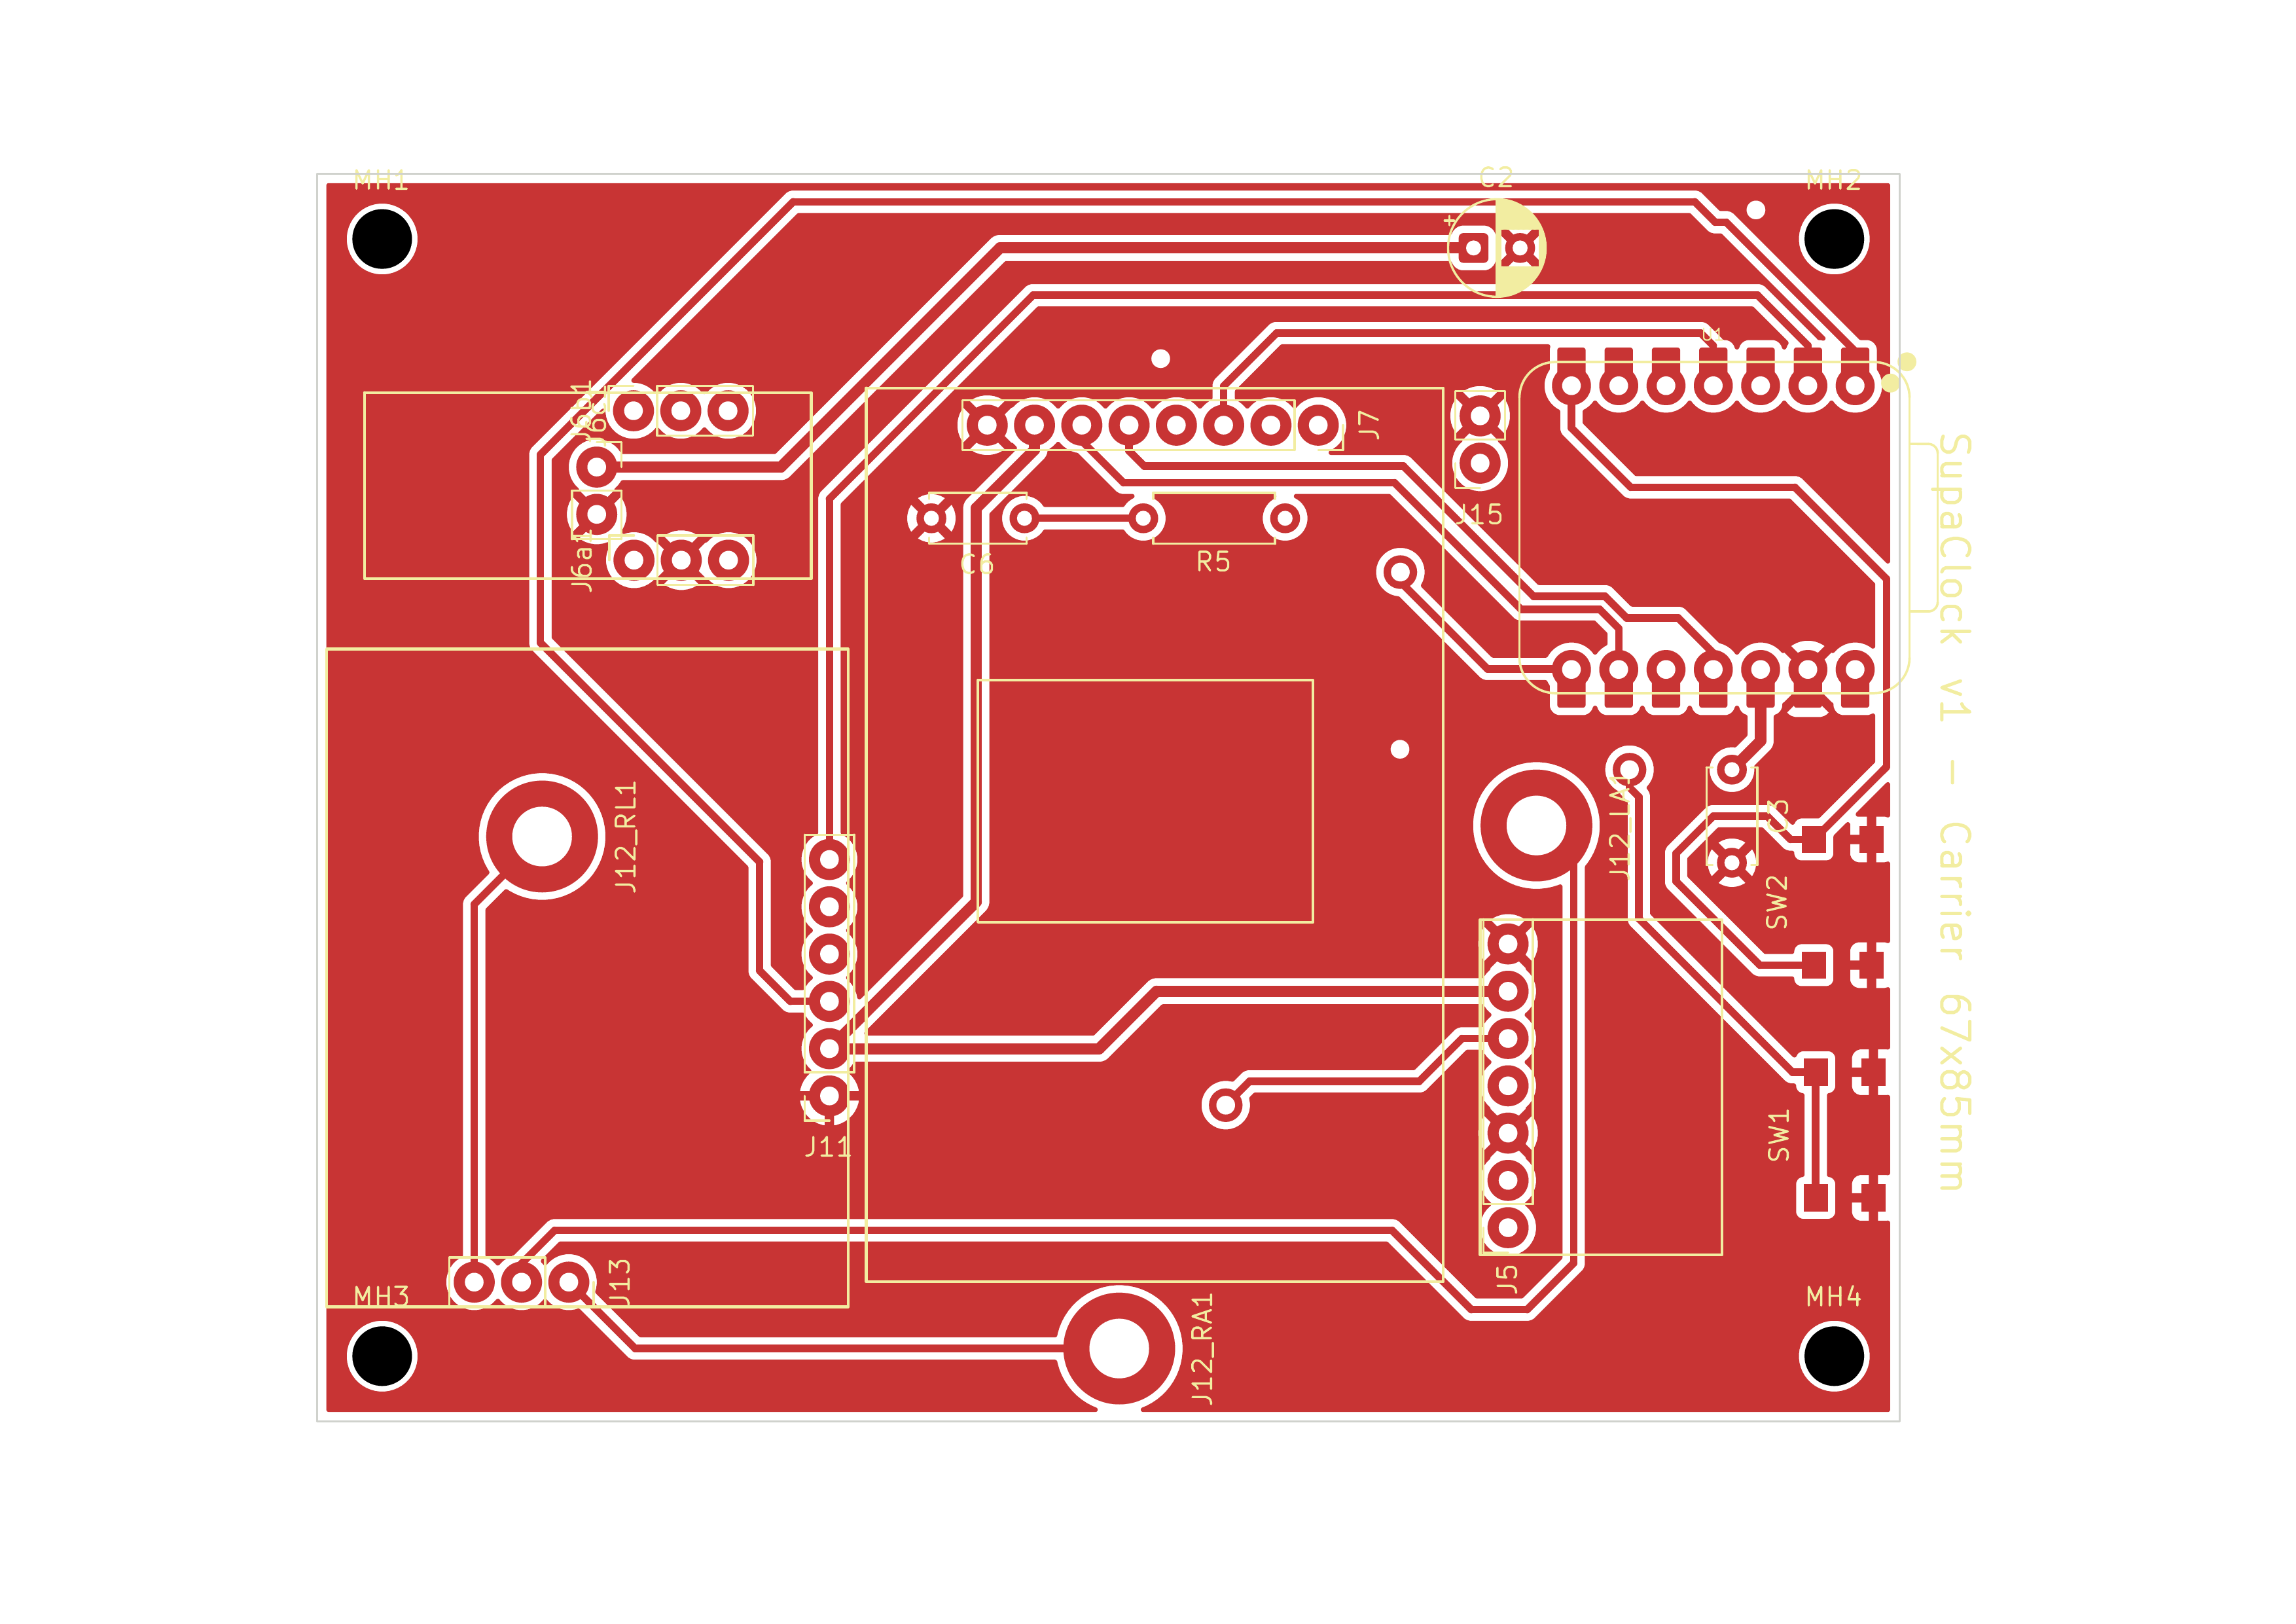
\includegraphics[width=\linewidth]{pcb_front-1.png}
        \caption{Trazado de cobre y distribución de componentes en la cara superior (Top) del Carrier v1.}
        \label{fig:pcb_front}
    \end{minipage}\hfill
    \begin{minipage}{0.48\textwidth}
        \centering
        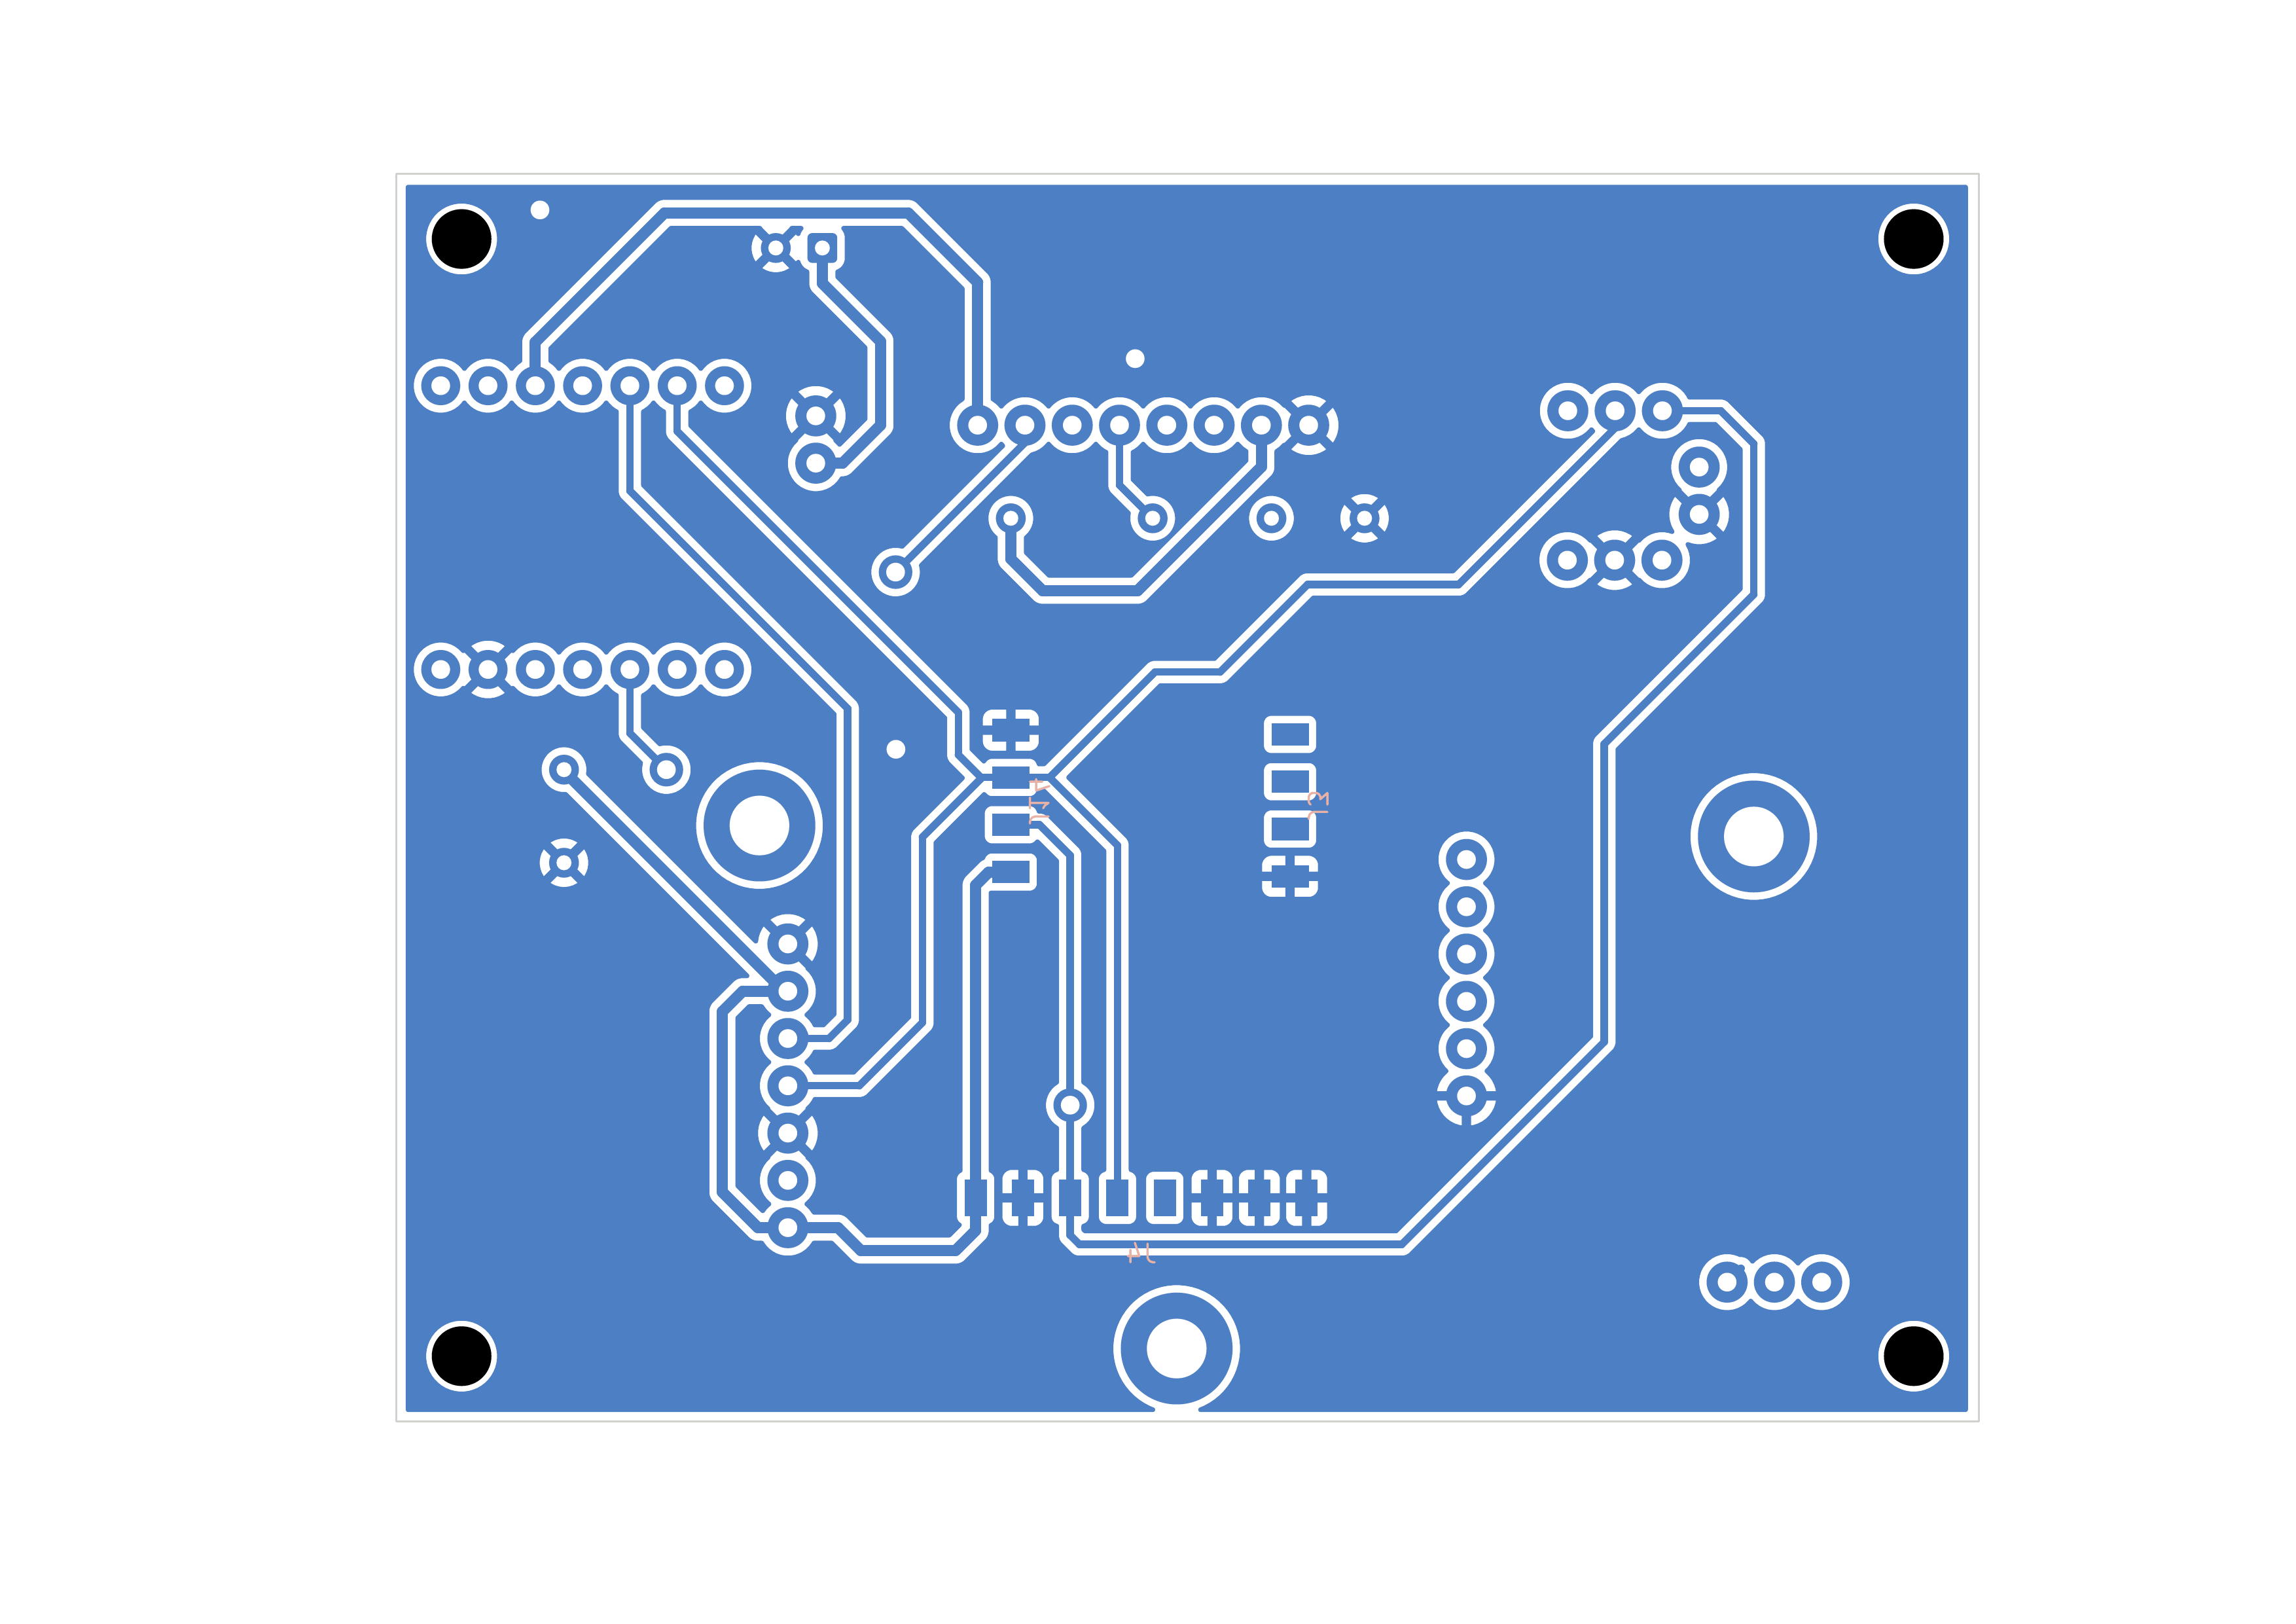
\includegraphics[width=\linewidth]{pcb_back-1.png}
        \caption{Trazado de cobre y cutouts para sensores en la cara inferior (Bottom) del Carrier v1.}
        \label{fig:pcb_back}
    \end{minipage}
\end{figure}

\begin{figure}[htbp]
    \centering
    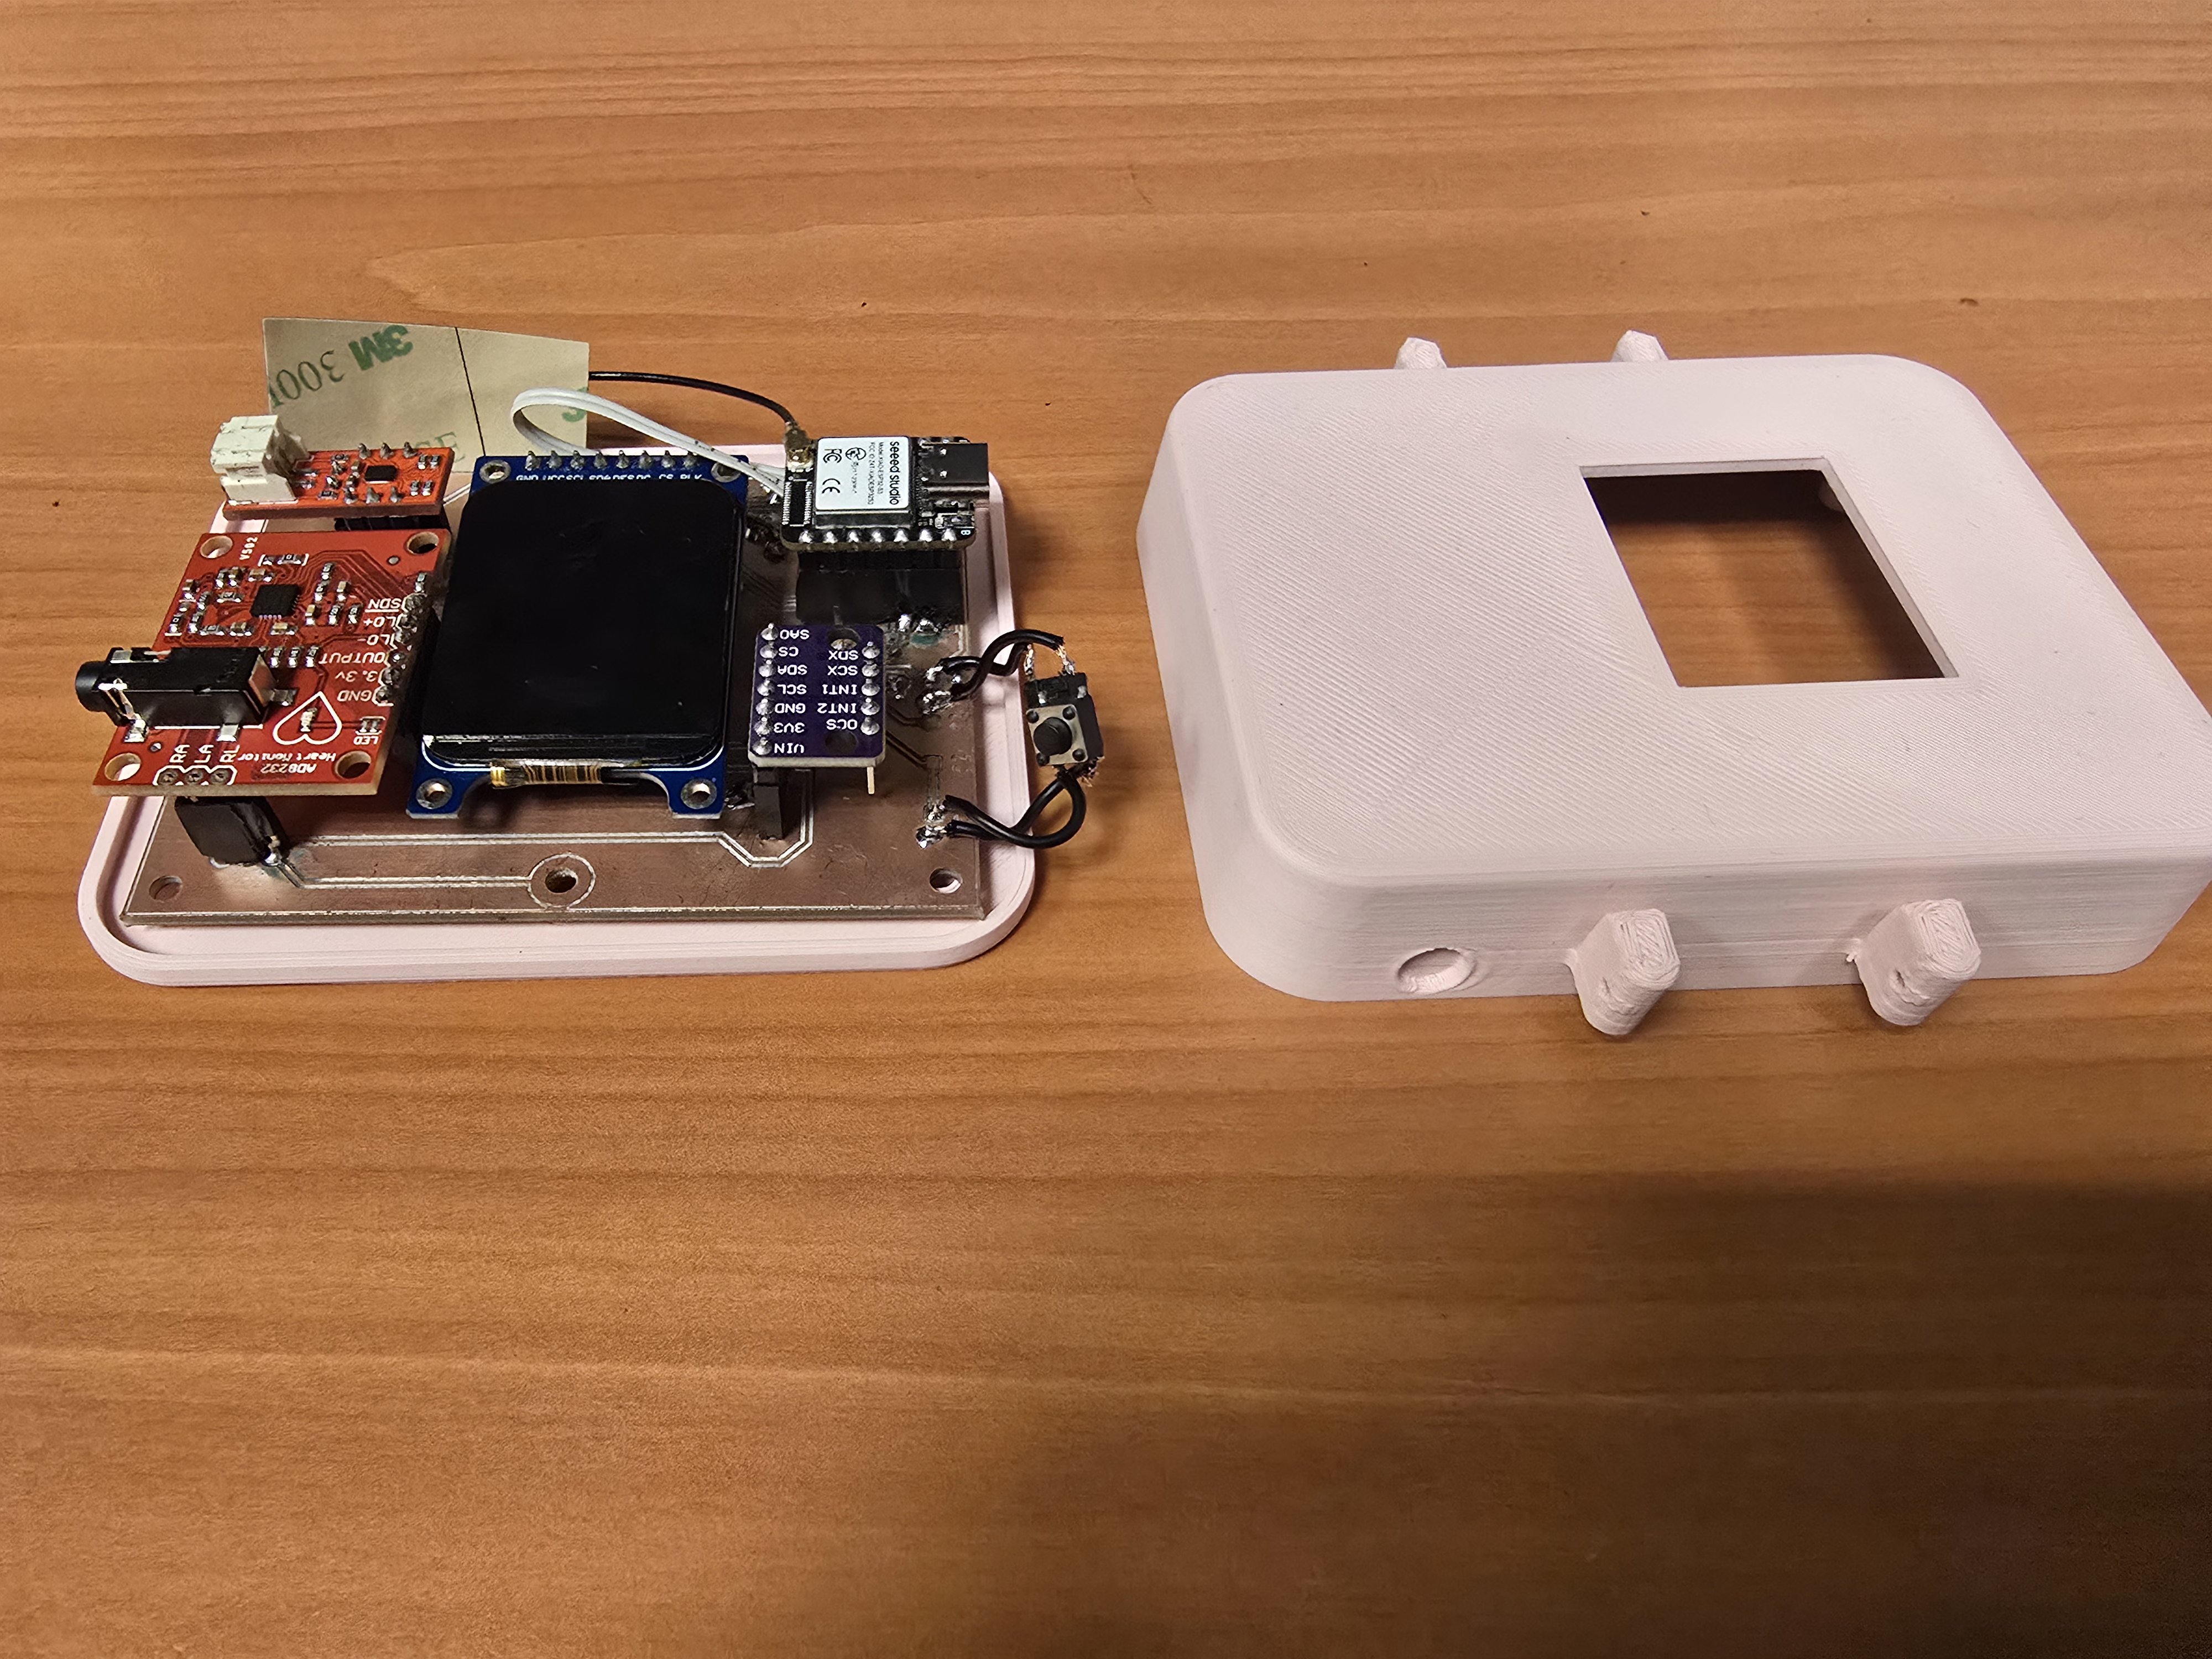
\includegraphics[width=0.78\textwidth,keepaspectratio]{prototipopcb.png}
    \caption{Prototipo físico: PCB Carrier v1 fresada y poblada con XIAO ESP32-S3, sensores en zócalos, AD8232 y display ST7789, asentada sobre la bottom case impresa de la carcasa V2. A la derecha, la top case impresa con su apertura para el display y los pilares de los botones, lista para el cierre del ensamble.}
    \label{fig:prototipo_pcb}
\end{figure}

\subsubsection{Placa adaptadora para pantalla de repuesto}

Durante el ensamble del Carrier v1 se detectó que la pantalla ST7789 originalmente integrada en la PCB principal presentaba un daño físico que comprometía su confiabilidad operativa. En lugar de retrabajar la PCB principal --- y poniendo en riesgo el resto de soldaduras ya validadas ---, el equipo decidió migrar a la unidad ST7789 de repuesto disponible en stock. Dado que el breakout del repuesto exponía un pinout y un footprint mecánico ligeramente distintos a los del modelo original, se diseñó y fabricó una pequeña PCB adaptadora dedicada cuya única función es reordenar las señales SPI (MOSI, SCK, CS, DC, RST, BLK) y proveer los puntos de fijación mecánicos correctos para la nueva pantalla, manteniendo intacto el ruteo del Carrier v1.

\textbf{Estado actual.} La PCB adaptadora ya está \textbf{fabricada por fresado en el FabLab}, pero \textbf{aún no se ha soldado}: la validación funcional de la pantalla de repuesto sobre el Carrier v1 queda como tarea inmediata en la lista de próximos pasos de la sección~\ref{sec:plan_validacion}, en paralelo a la campaña de captura de datos de la clase \textit{caída} del HAR.

\subsection{Carcasa protectora}

\subsubsection{Descripción}

Protección externa e interfaz física que aloja la electrónica del wearable, fabricada mediante impresión 3D.

\subsubsection{Decisiones de diseño y geometría}

La estructura de la carcasa incorpora esquinas redondeadas y un perfil cónico que maximiza la comodidad en la muñeca. La sujeción física de la correa utiliza ranuras de 20\,mm de ancho con orificio de 1,8\,mm para spring bar, integradas directamente en las paredes exteriores. Esta cota es la del estándar Samsung Galaxy Watch 4/5/6, lo que permite reutilizar directamente cualquier correa comercial de ese ecosistema sin tener que fabricar una a medida.

El cuerpo se divide en dos secciones para facilitar el armado y mantenimiento. Se definieron aperturas superiores para la pantalla y ranuras en la base inferior para asegurar el contacto de los sensores ópticos, de temperatura y los electrodos de acero inoxidable para la medición del ECG.

\subsubsection{Iteración tras impresión}

La primera versión impresa reveló problemas de espacio para albergar la Seeed S3 y la batería juntas en el interior, además de que el footprint físico real de los botones difería levemente de la PCB. Se validó que el cutout del sensor MAX30102 era geométricamente correcto desde el inicio, descartando errores de orientación. El equipo incrementó la profundidad de los orificios laterales a 16\,mm para cruzar por completo las paredes curvas, e inició un rediseño del contorno y pilares para la siguiente iteración física con holguras mecánicas mejoradas.

\subsubsection{Resultados}

\begin{itemize}
    \item Segunda versión de carcasa paramétrica impresa en PLA FDM, logrando un acoplamiento mecánico adecuado con el carrier PCB.
    \item Se verificó el correcto recorrido de los pulsadores mecánicos (button caps) y la accesibilidad al conector USB lateral.
    \item Se determinó la necesidad de añadir orificios mecánicos específicos y ensanchar 1,5\,mm el volumen interno en la siguiente iteración para facilitar el paso y fijación de los pernos de la pantalla.
\end{itemize}

La \textbf{carcasa V2 es la versión final del avance 3}: cierra el bloque mecánico para esta entrega y queda como envolvente físico oficial del prototipo integrado. El trabajo sobre la \textbf{V3} comenzará a continuación del cierre de este informe, incorporando las correcciones listadas (orificios para los pernos de la pantalla, ensanchamiento de 1,5\,mm del volumen interno, ajuste del footprint de los botones tras la próxima iteración del Carrier, y \textbf{descenso de los orificios del spring bar al borde inferior de los lugs} para aprovechar el recorrido completo de las correas Galaxy Watch y evitar el pliegue de la correa contra el chasis).

\begin{figure}[H]
    \centering
    \begin{minipage}{0.48\textwidth}
        \centering
        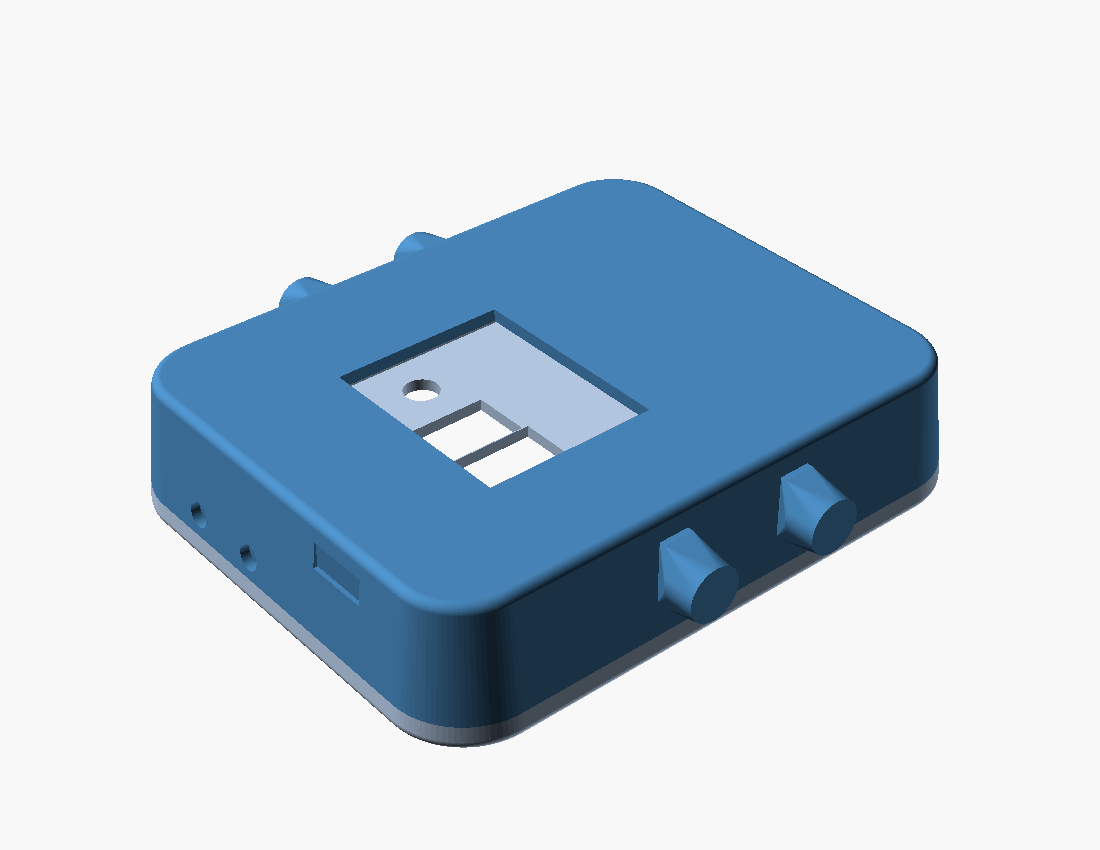
\includegraphics[width=\linewidth]{render_v2_assembly_hero.png}
        \caption{Ensamble conceptual completo de la carcasa V2 mostrando el top case, bottom case y los button caps.}
        \label{fig:render_hero}
    \end{minipage}\hfill
    \begin{minipage}{0.48\textwidth}
        \centering
        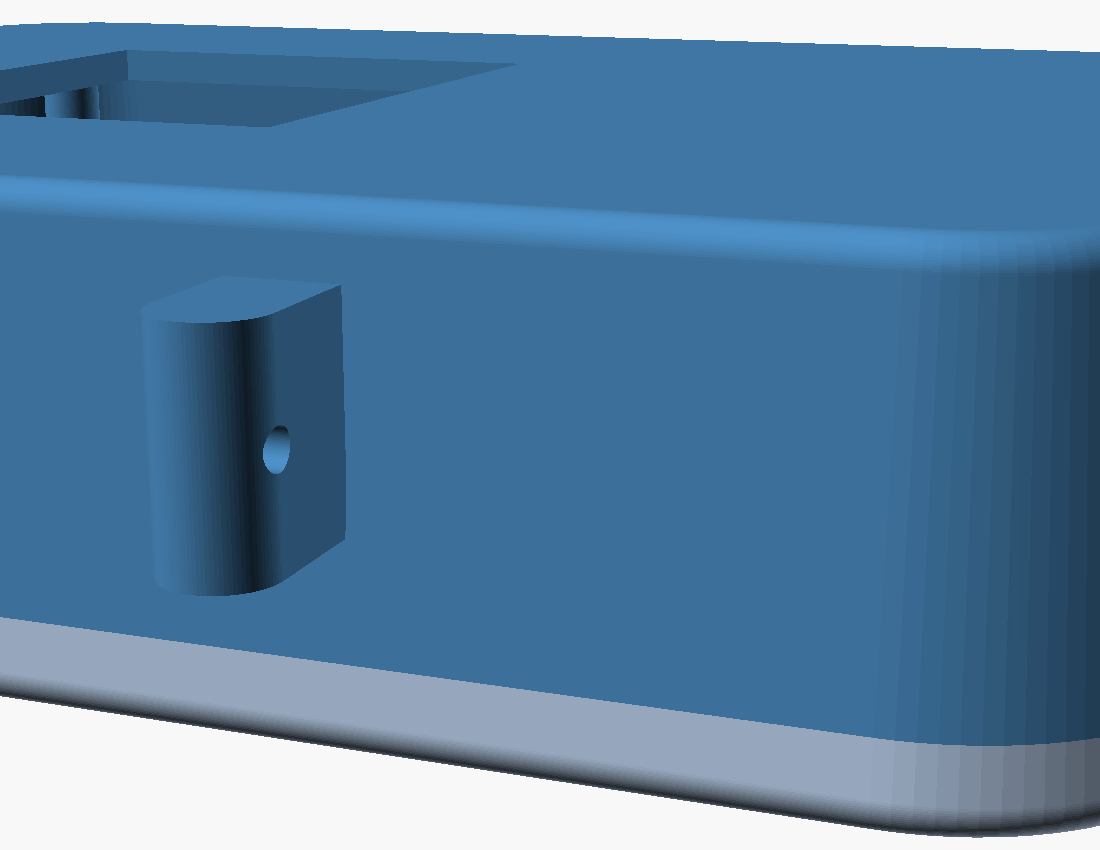
\includegraphics[width=\linewidth]{render_v2_lug_closeup.png}
        \caption{Detalle de los lugs tipo stadium con ancho de 20\,mm y orificio de 1,8\,mm compatible con spring bar estándar Samsung Galaxy Watch.}
        \label{fig:render_lug}
    \end{minipage}
\end{figure}

\begin{figure}[htbp]
    \centering
    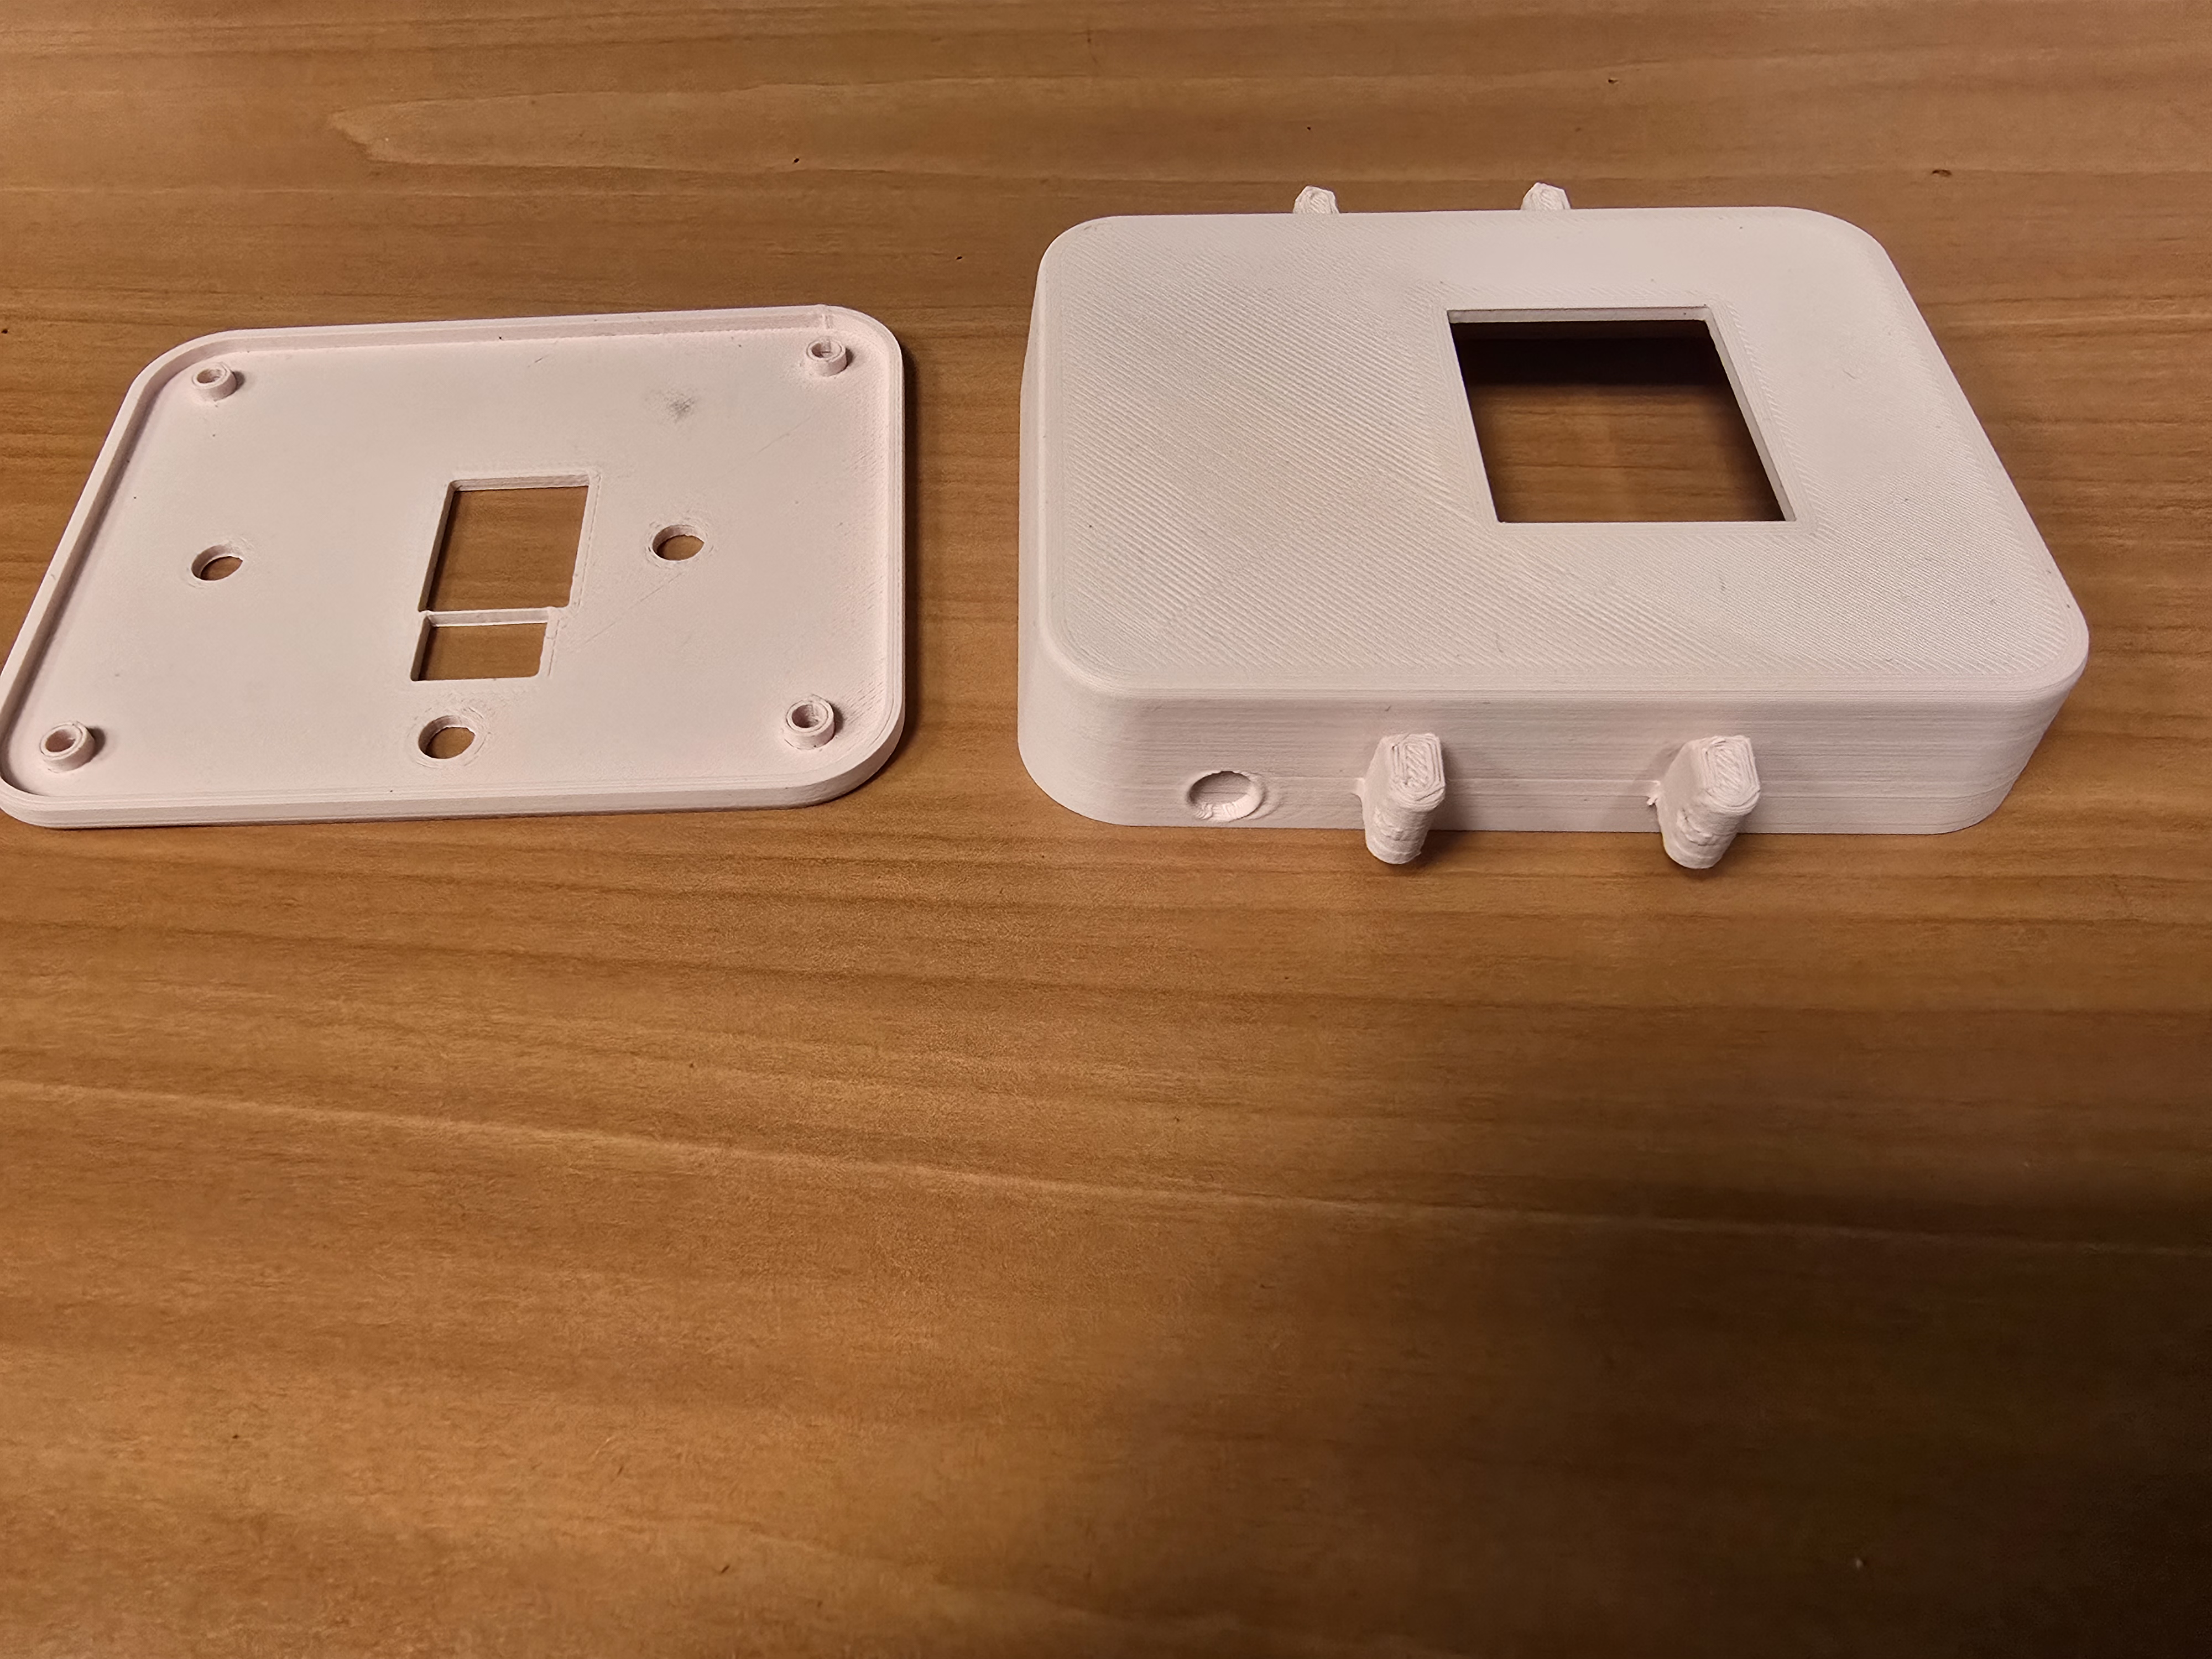
\includegraphics[width=0.78\textwidth,keepaspectratio]{carcasas.png}
    \caption{Carcasa V2 impresa en PLA: bottom case (izquierda) con los cuatro orificios para los pernos M3 de cierre y el cutout central para la pantalla, y top case (derecha) con su apertura para el display y los dos pilares cilíndricos de los button caps que transmiten la pulsación a la PCB.}
    \label{fig:carcasas_impresas}
\end{figure}

\subsection{Aplicación móvil Flutter}

\subsubsection{Descripción}

Desarrollo e implementación de la app móvil en el directorio \texttt{app/} utilizando Flutter 3.24 y Dart 3.5, desempeñando el rol de gateway BLE, osciloscopio en tiempo real, registrador inercial y dashboard del usuario, operando con una filosofía offline-first.

\subsubsection{Arquitectura de servicios singleton}

Los servicios del backend local en Dart se estructuran bajo un patrón de diseño Singleton, garantizando canales de comunicación únicos y seguros:
\begin{itemize}
    \item \textbf{Autenticación (\texttt{auth\_service.dart}):} Inicializa y gestiona las sesiones de usuario con Firebase Auth de manera reactiva, manteniendo el estado de ingreso seguro.
    \item \textbf{Comunicación BLE (\texttt{ble\_service.dart}):} Controla el ciclo de vida del enlace inalámbrico (escaneo, conexión, sincronización MTU y reconexión automática) a través del canal de notificaciones BLE, decodificando las tramas TLV entrantes.
    \item \textbf{Registro de señales (\texttt{csv\_recorder.dart}):} Encargado de empaquetar, estructurar en CSV, comprimir con algoritmo gzip y subir asíncronamente las señales continuas al Storage de Firebase, optimizando el ancho de banda.
    \item \textbf{Resúmenes biométricos (\texttt{daily\_rollup\_service.dart}):} Computa de forma local y asíncrona las tendencias diarias acumuladas del usuario.
    \item \textbf{Caché local (\texttt{local\_store.dart}):} Implementa persistencia instantánea basada en la base de datos local Hive para una experiencia offline fluida.
    \item \textbf{Notificaciones (\texttt{notifications\_service.dart}):} Administra las alarmas físicas locales de salud en el celular tras detectar anomalías críticas.
    \item \textbf{Procesamiento ECG (\texttt{pan\_tompkins.dart}):} Ejecuta en un isolate asíncrono de Dart (contexto Thread-Safe independiente del UI thread) el algoritmo QRS para calcular la frecuencia cardíaca instantánea y métricas de HRV directamente en el teléfono.
    \item \textbf{Sincronización remota (\texttt{firestore\_service.dart}):} Centraliza lectura/escritura contra Firestore, garantizando que los \textit{rollups} y eventos clínicos del usuario queden replicados en la nube cuando hay conectividad.
    \item \textbf{Recolección de telemetría (\texttt{telemetry\_collector.dart}):} Enruta los \textit{snapshots} TLV agregados del firmware hacia los demás servicios (caché local, dashboard reactivo y subidas asíncronas), actuando como bus interno de la app.
\end{itemize}

\subsubsection{Doble interfaz y menús detallados}

La aplicación móvil ofrece una interfaz en español dividida en dos modos principales:
\begin{enumerate}
    \item \textbf{Modo de Usuario Final:} Diseñado bajo lineamientos ergonómicos. Provee un dashboard que visualiza la telemetría en tiempo real (batería, pasos, HRV actual), una sección de spot-checks para iniciar lecturas puntuales de 30 segundos, y pantallas de tendencias históricas diarias.
    \item \textbf{Modo de Desarrollo / Depuración:} Oculto tras 7 pulsaciones consecutivas sobre el indicador de versión en el perfil del usuario. Expone osciloscopios gráficos de alta velocidad en tiempo real para aceleración ($a_x, a_y, a_z$) y ECG, una consola de depuración para inyección manual de comandos BLE, y la herramienta de captura CSV local para entrenar el modelo ML.
\end{enumerate}

Las figuras \ref{fig:screenshots_user} y \ref{fig:screenshots_dev} reúnen las ocho vistas reales de la aplicación, separadas por modo: las cuatro de usuario final (\rfigura{fig:screenshots_user}) cubren el flujo cotidiano de consulta de biométricas, y las cuatro del modo desarrollador (\rfigura{fig:screenshots_dev}) detallan las herramientas de depuración e ingeniería del firmware.

\begin{figure}[htbp]
    \centering
    \begin{minipage}{0.235\textwidth}
        \centering
        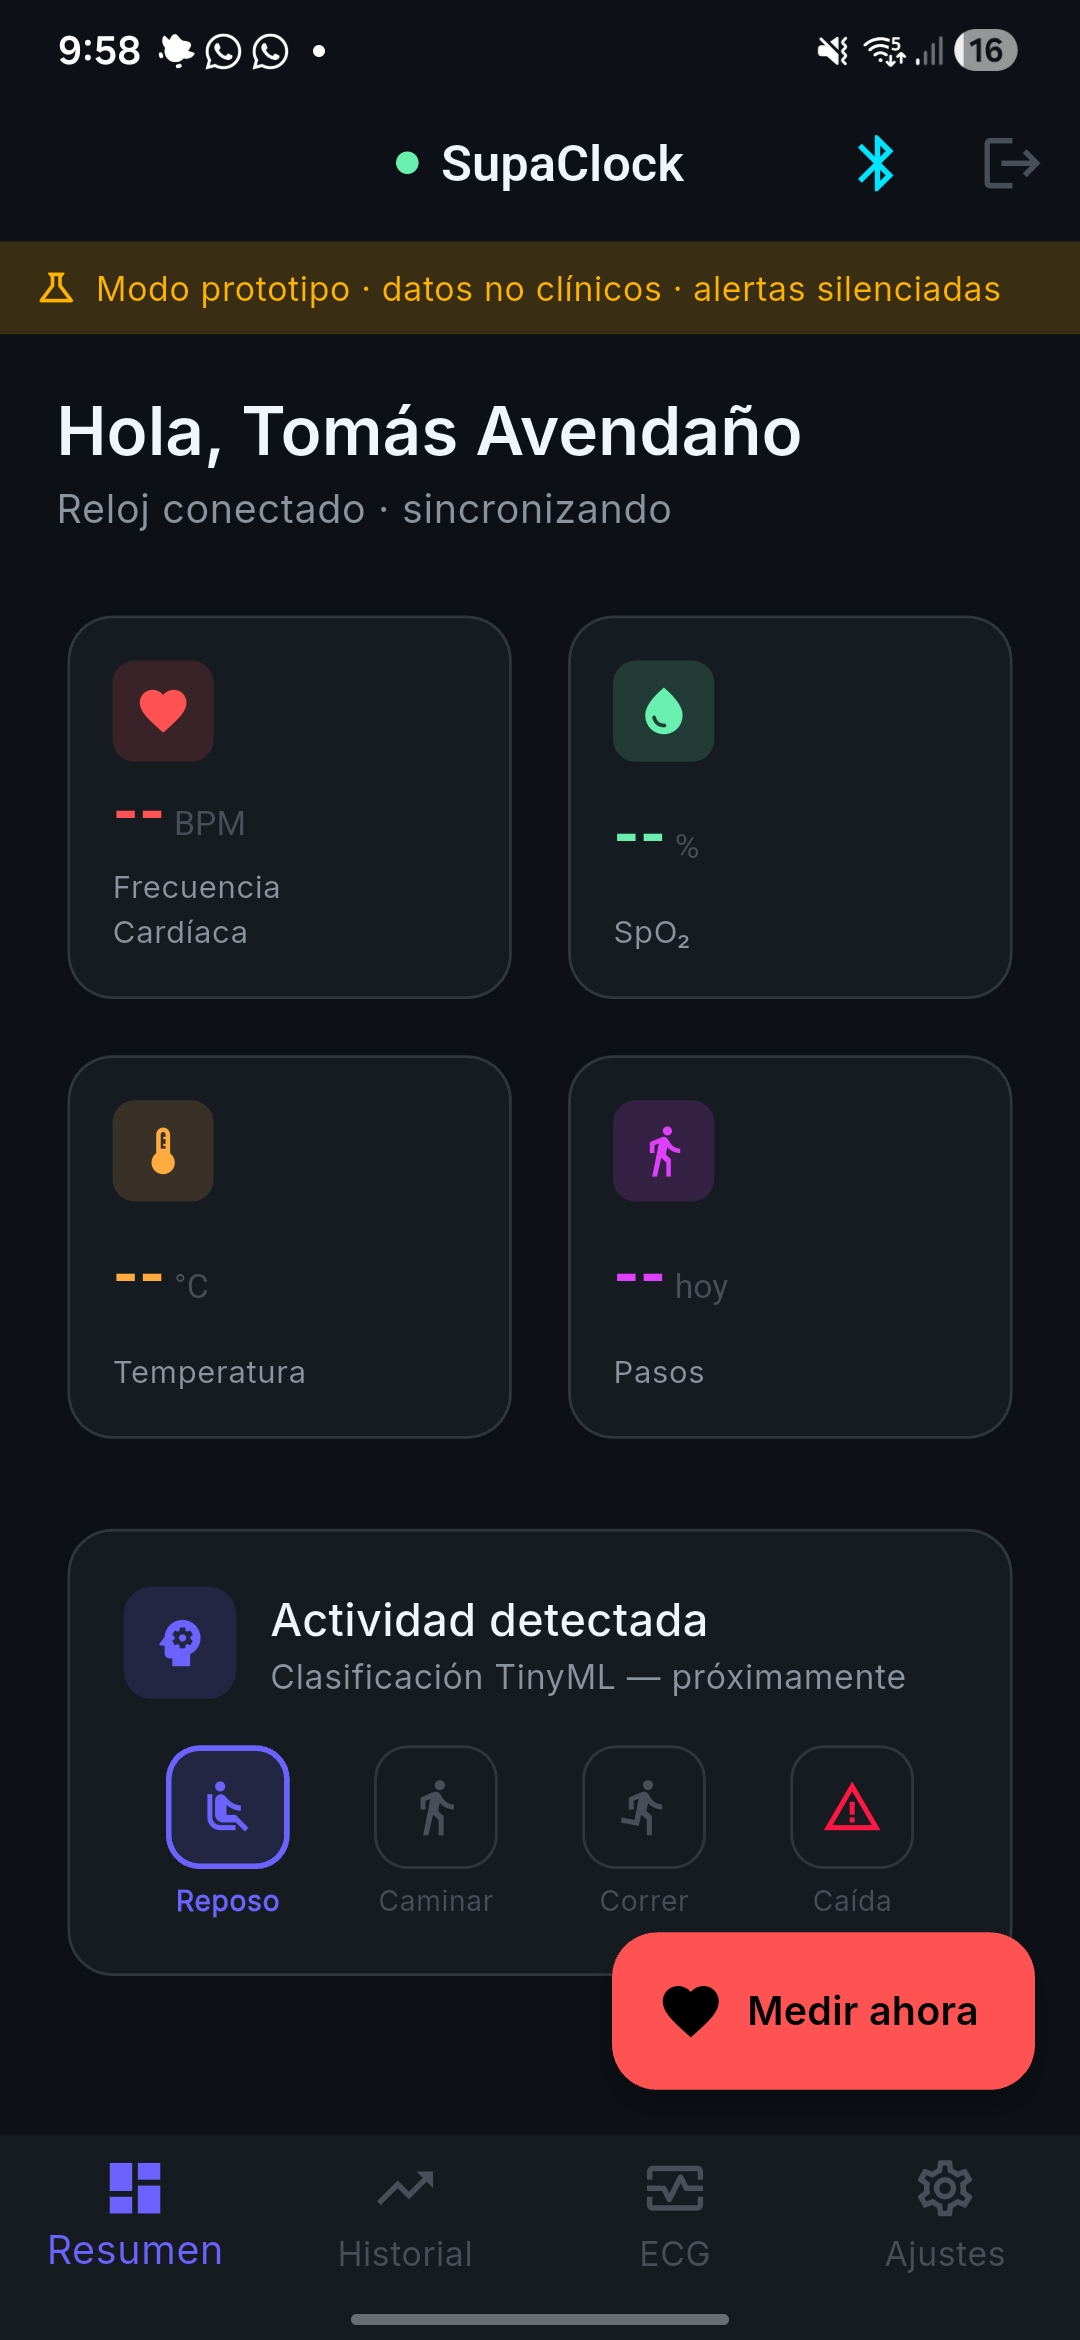
\includegraphics[width=\linewidth,keepaspectratio]{Screenshot_20260601_215805.jpg.jpeg}
        \subcaption{Resumen: tarjetas de Frecuencia Cardíaca, SpO\textsubscript{2}, Temperatura y Pasos, clasificación TinyML y CTA «Medir ahora».}
        \label{fig:ss_home}
    \end{minipage}\hfill
    \begin{minipage}{0.235\textwidth}
        \centering
        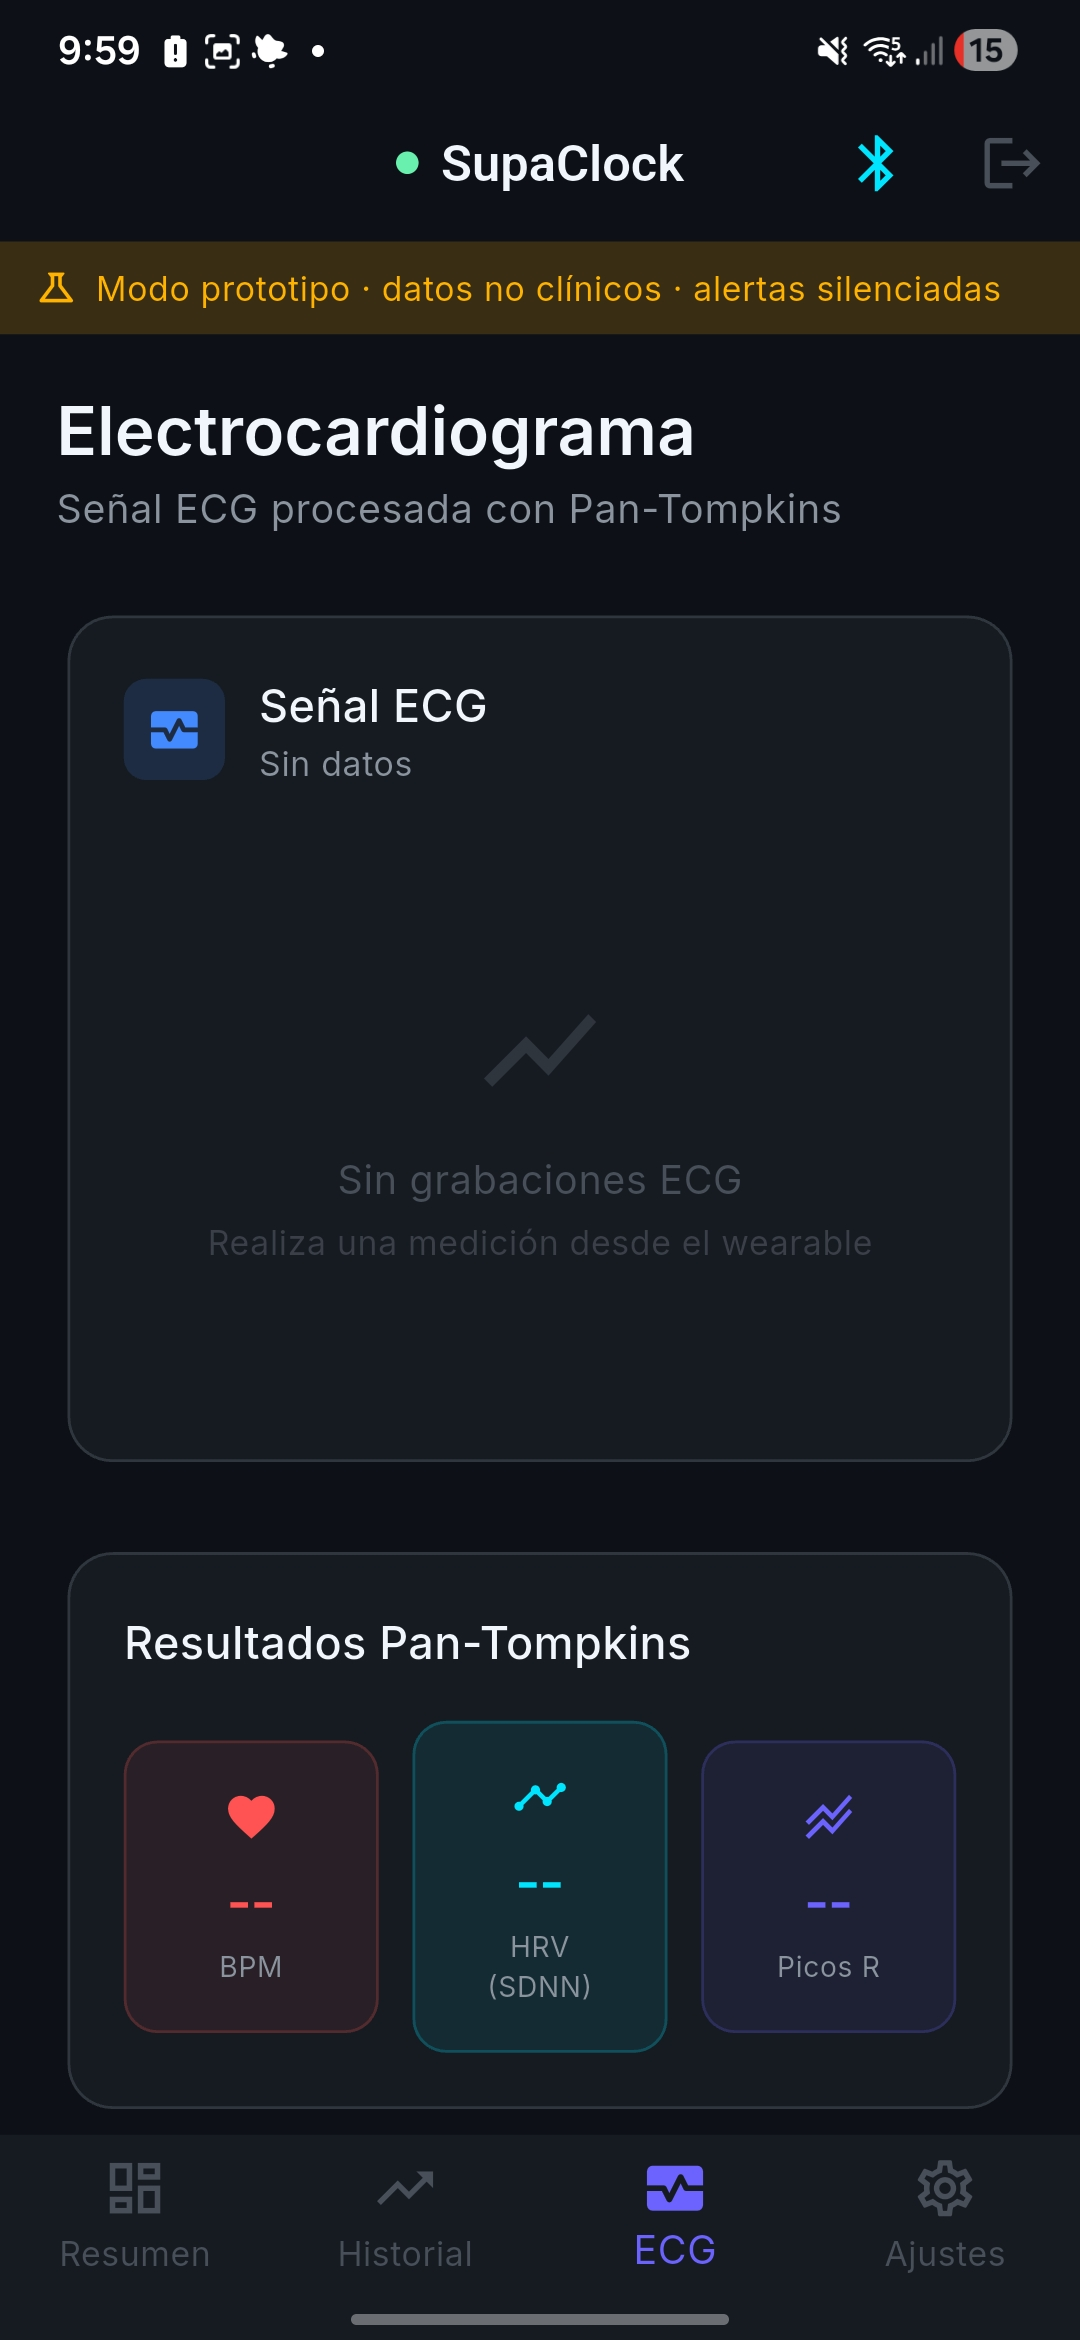
\includegraphics[width=\linewidth,keepaspectratio]{Screenshot_20260601_215907.jpg.jpeg}
        \subcaption{Electrocardiograma: señal procesada con Pan-Tompkins y resultados BPM, HRV (SDNN) y conteo de picos R.}
        \label{fig:ss_ecg_user}
    \end{minipage}\hfill
    \begin{minipage}{0.235\textwidth}
        \centering
        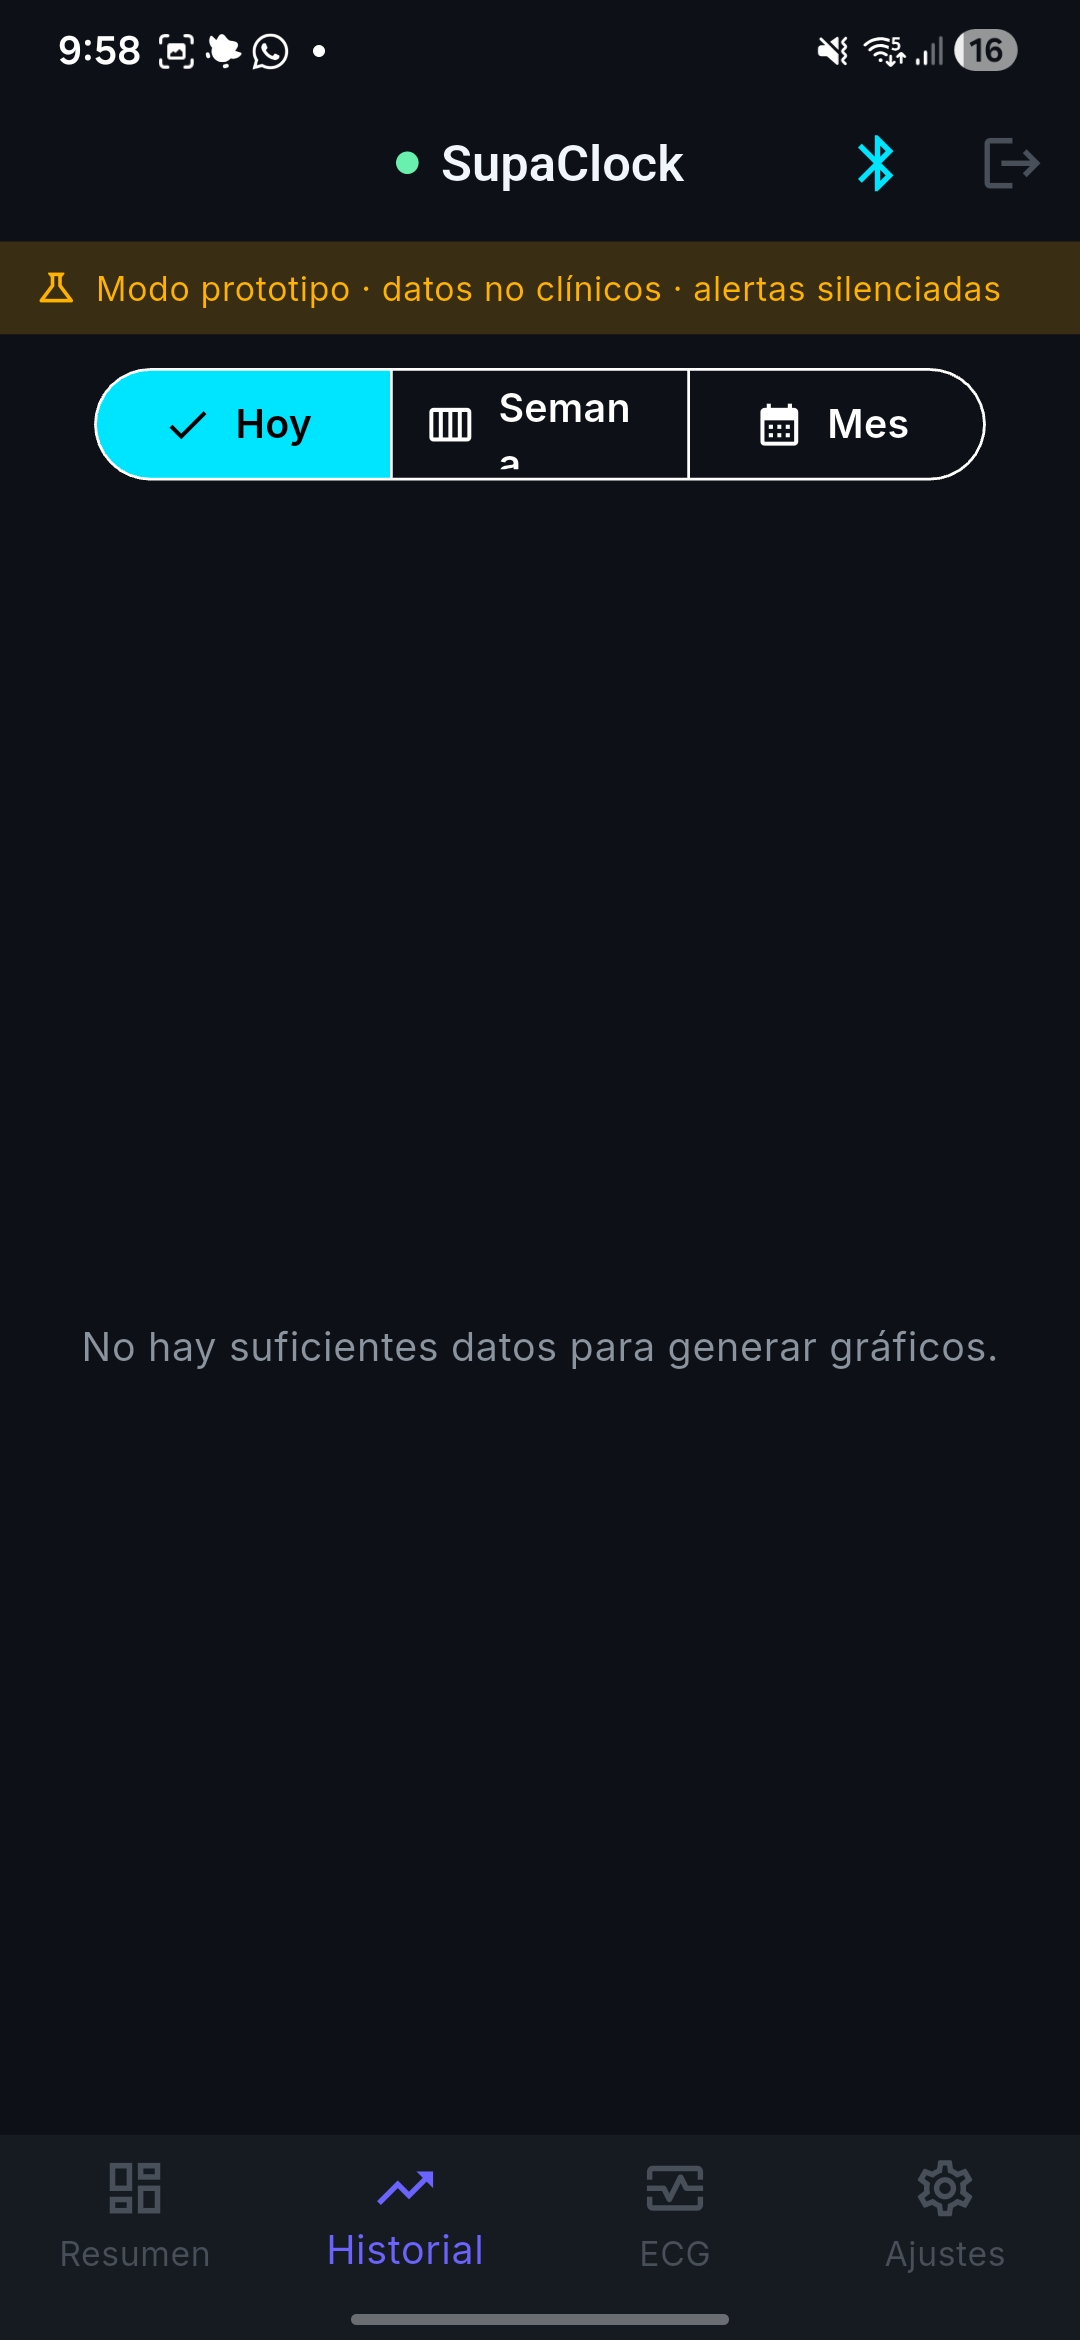
\includegraphics[width=\linewidth,keepaspectratio]{Screenshot_20260601_215856.jpg.jpeg}
        \subcaption{Historial: filtros Hoy/Semana/Mes con placeholder cuando aún no hay datos consolidados.}
        \label{fig:ss_hist}
    \end{minipage}\hfill
    \begin{minipage}{0.235\textwidth}
        \centering
        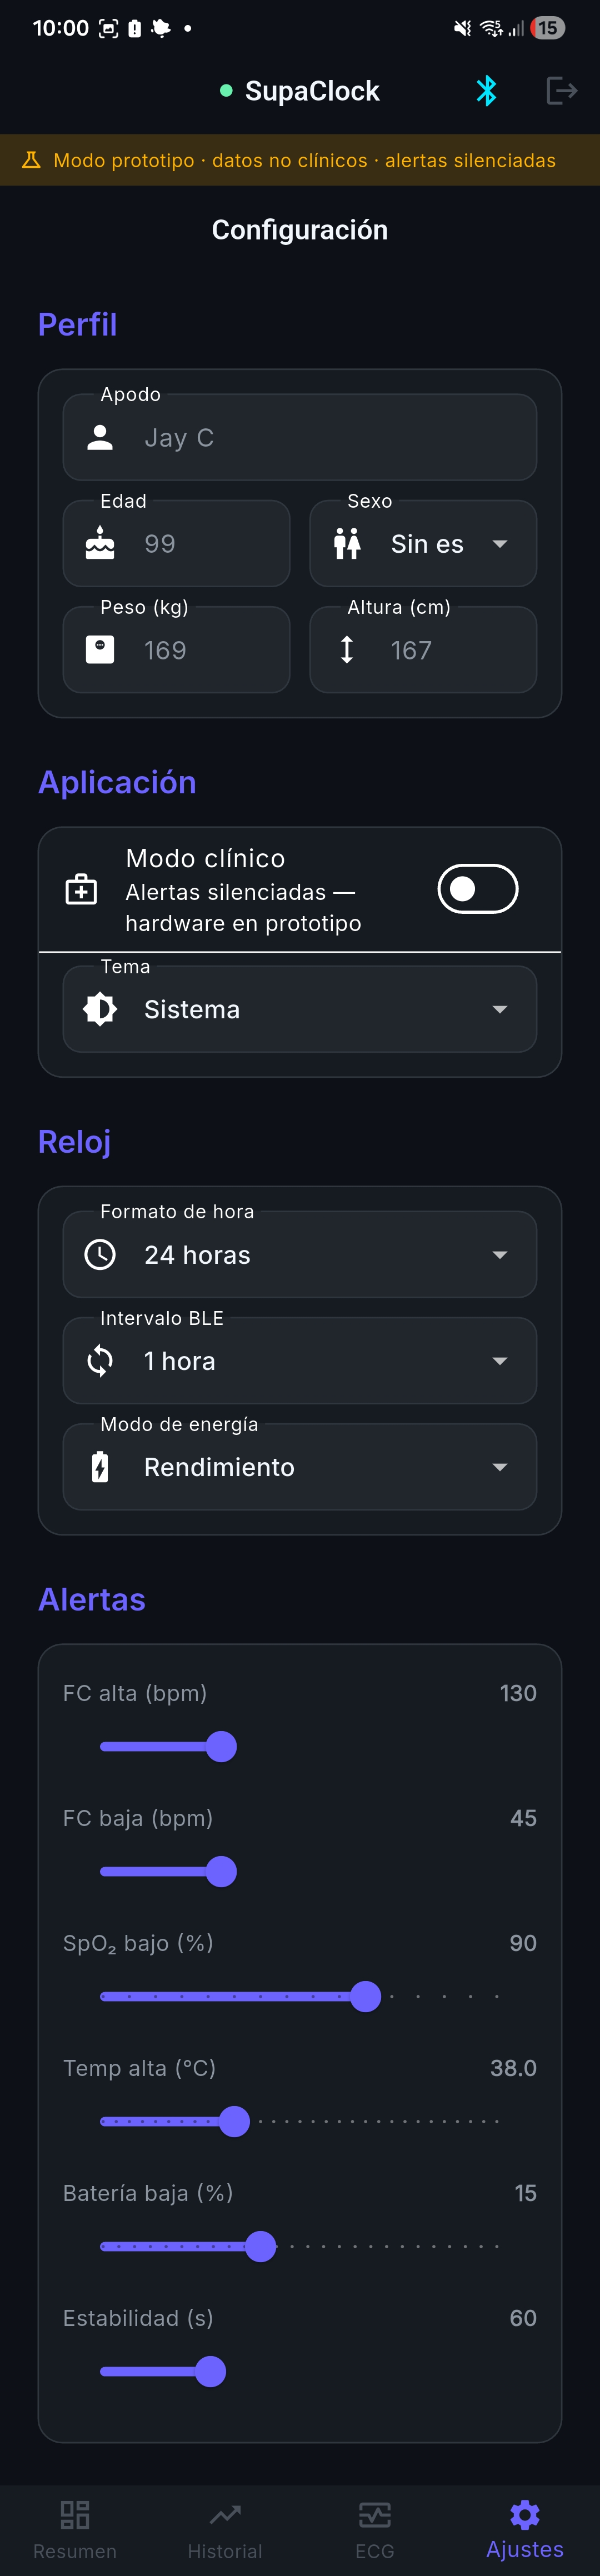
\includegraphics[width=\linewidth,keepaspectratio]{Screenshot_20260601_220001.jpg.jpeg}
        \subcaption{Ajustes: perfil, modo clínico, tema visual, formato de hora, intervalo BLE, modo de energía y umbrales de alerta.}
        \label{fig:ss_settings}
    \end{minipage}
    \caption{Vistas del modo Usuario Final de la aplicación móvil Flutter.}
    \label{fig:screenshots_user}
\end{figure}

\begin{figure}[htbp]
    \centering
    \begin{minipage}{0.235\textwidth}
        \centering
        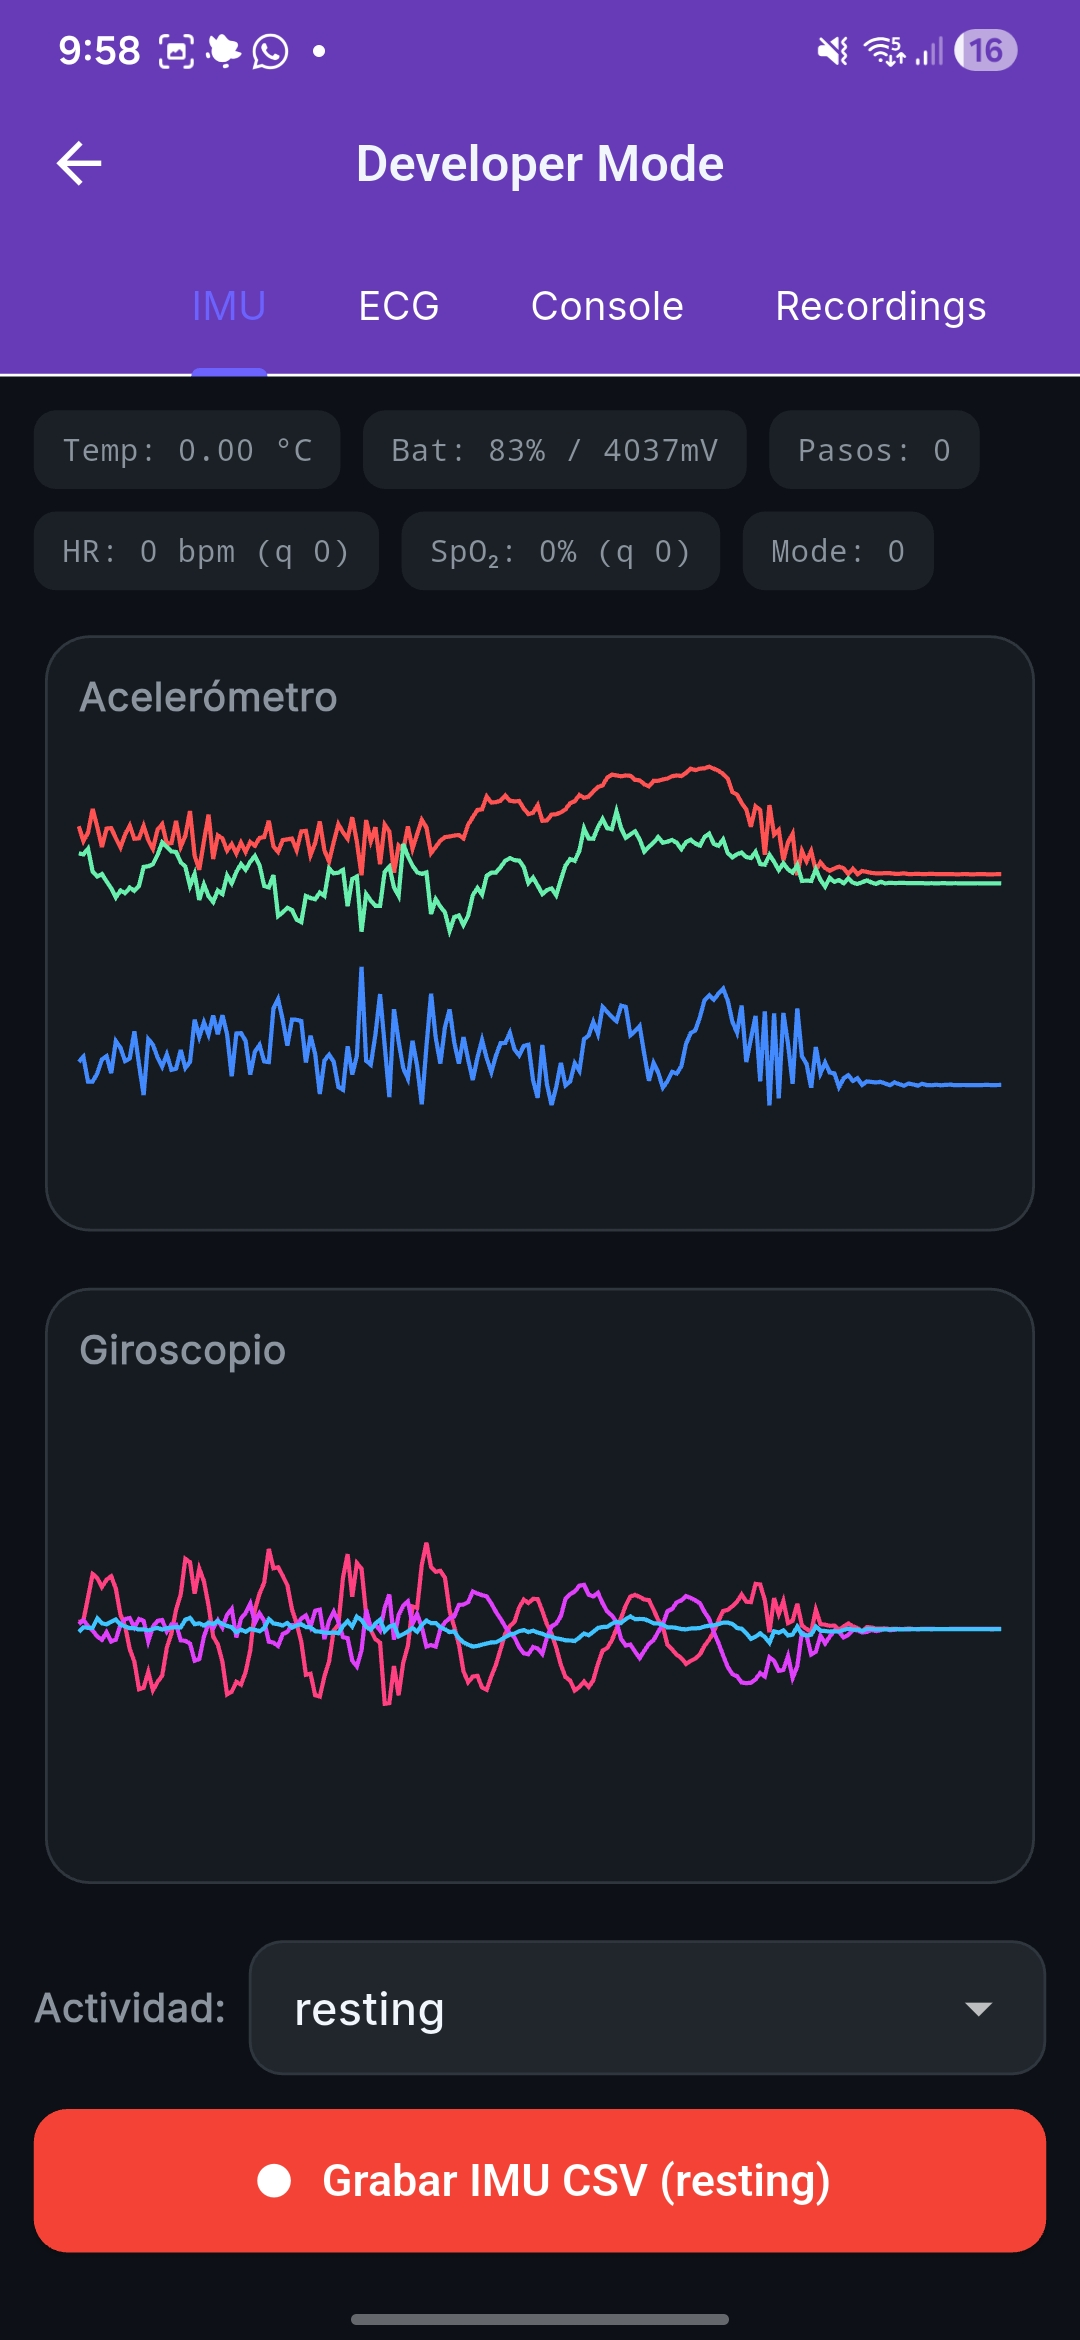
\includegraphics[width=\linewidth,keepaspectratio]{Screenshot_20260601_215834.jpg.jpeg}
        \subcaption{Dev $\rightarrow$ IMU: osciloscopios en tiempo real del acelerómetro y giroscopio del BMI160 más cabecera de telemetría (Temp, batería, HR, SpO\textsubscript{2}).}
        \label{fig:ss_dev_imu}
    \end{minipage}\hfill
    \begin{minipage}{0.235\textwidth}
        \centering
        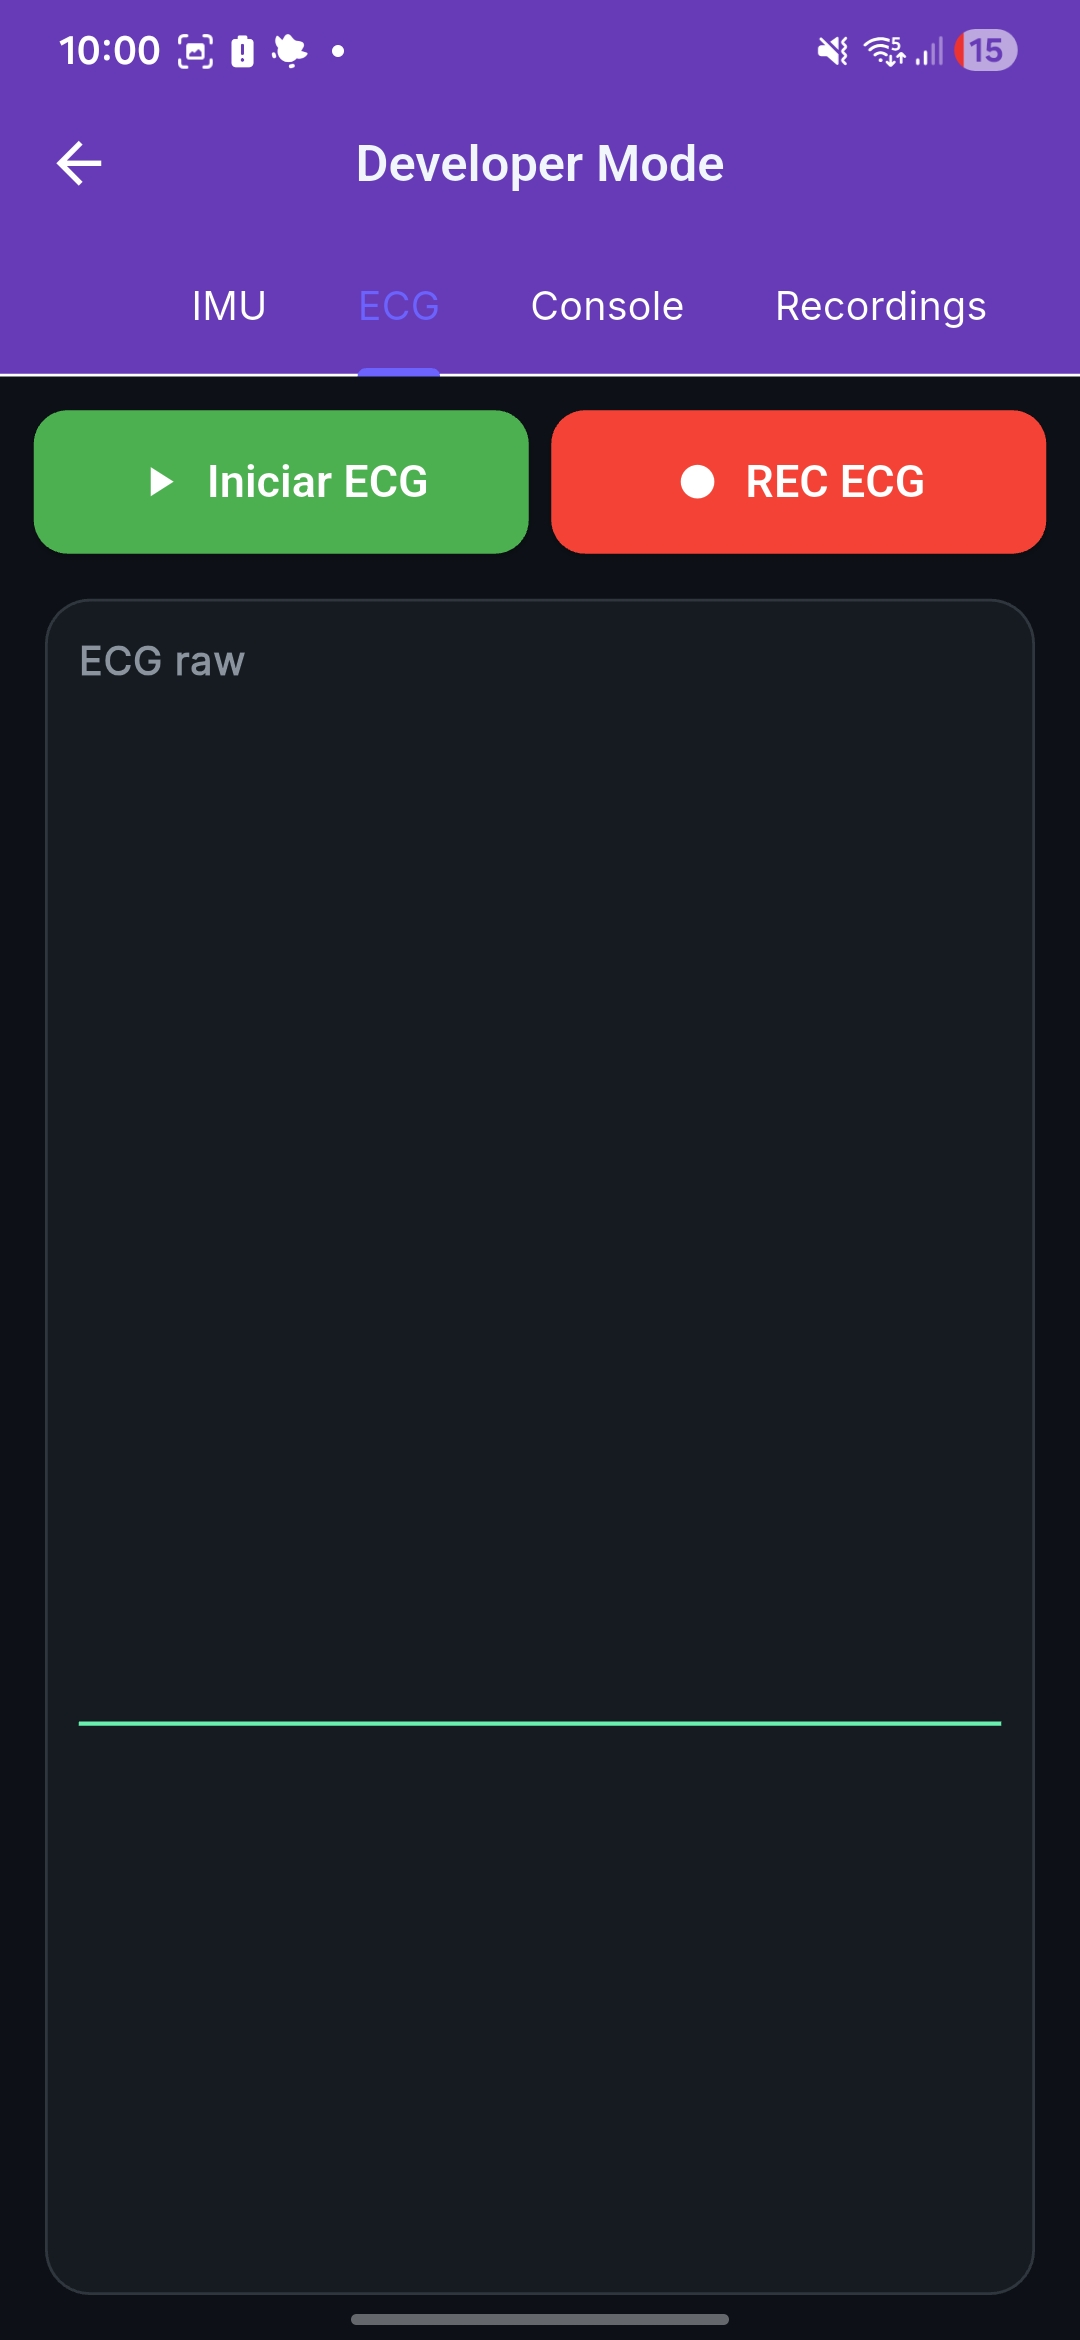
\includegraphics[width=\linewidth,keepaspectratio]{Screenshot_20260601_220039.jpg.jpeg}
        \subcaption{Dev $\rightarrow$ ECG: control de captura (Iniciar/REC) y visor de la señal cruda del AD8232 vía característica BLE 0xFF03.}
        \label{fig:ss_dev_ecg}
    \end{minipage}\hfill
    \begin{minipage}{0.235\textwidth}
        \centering
        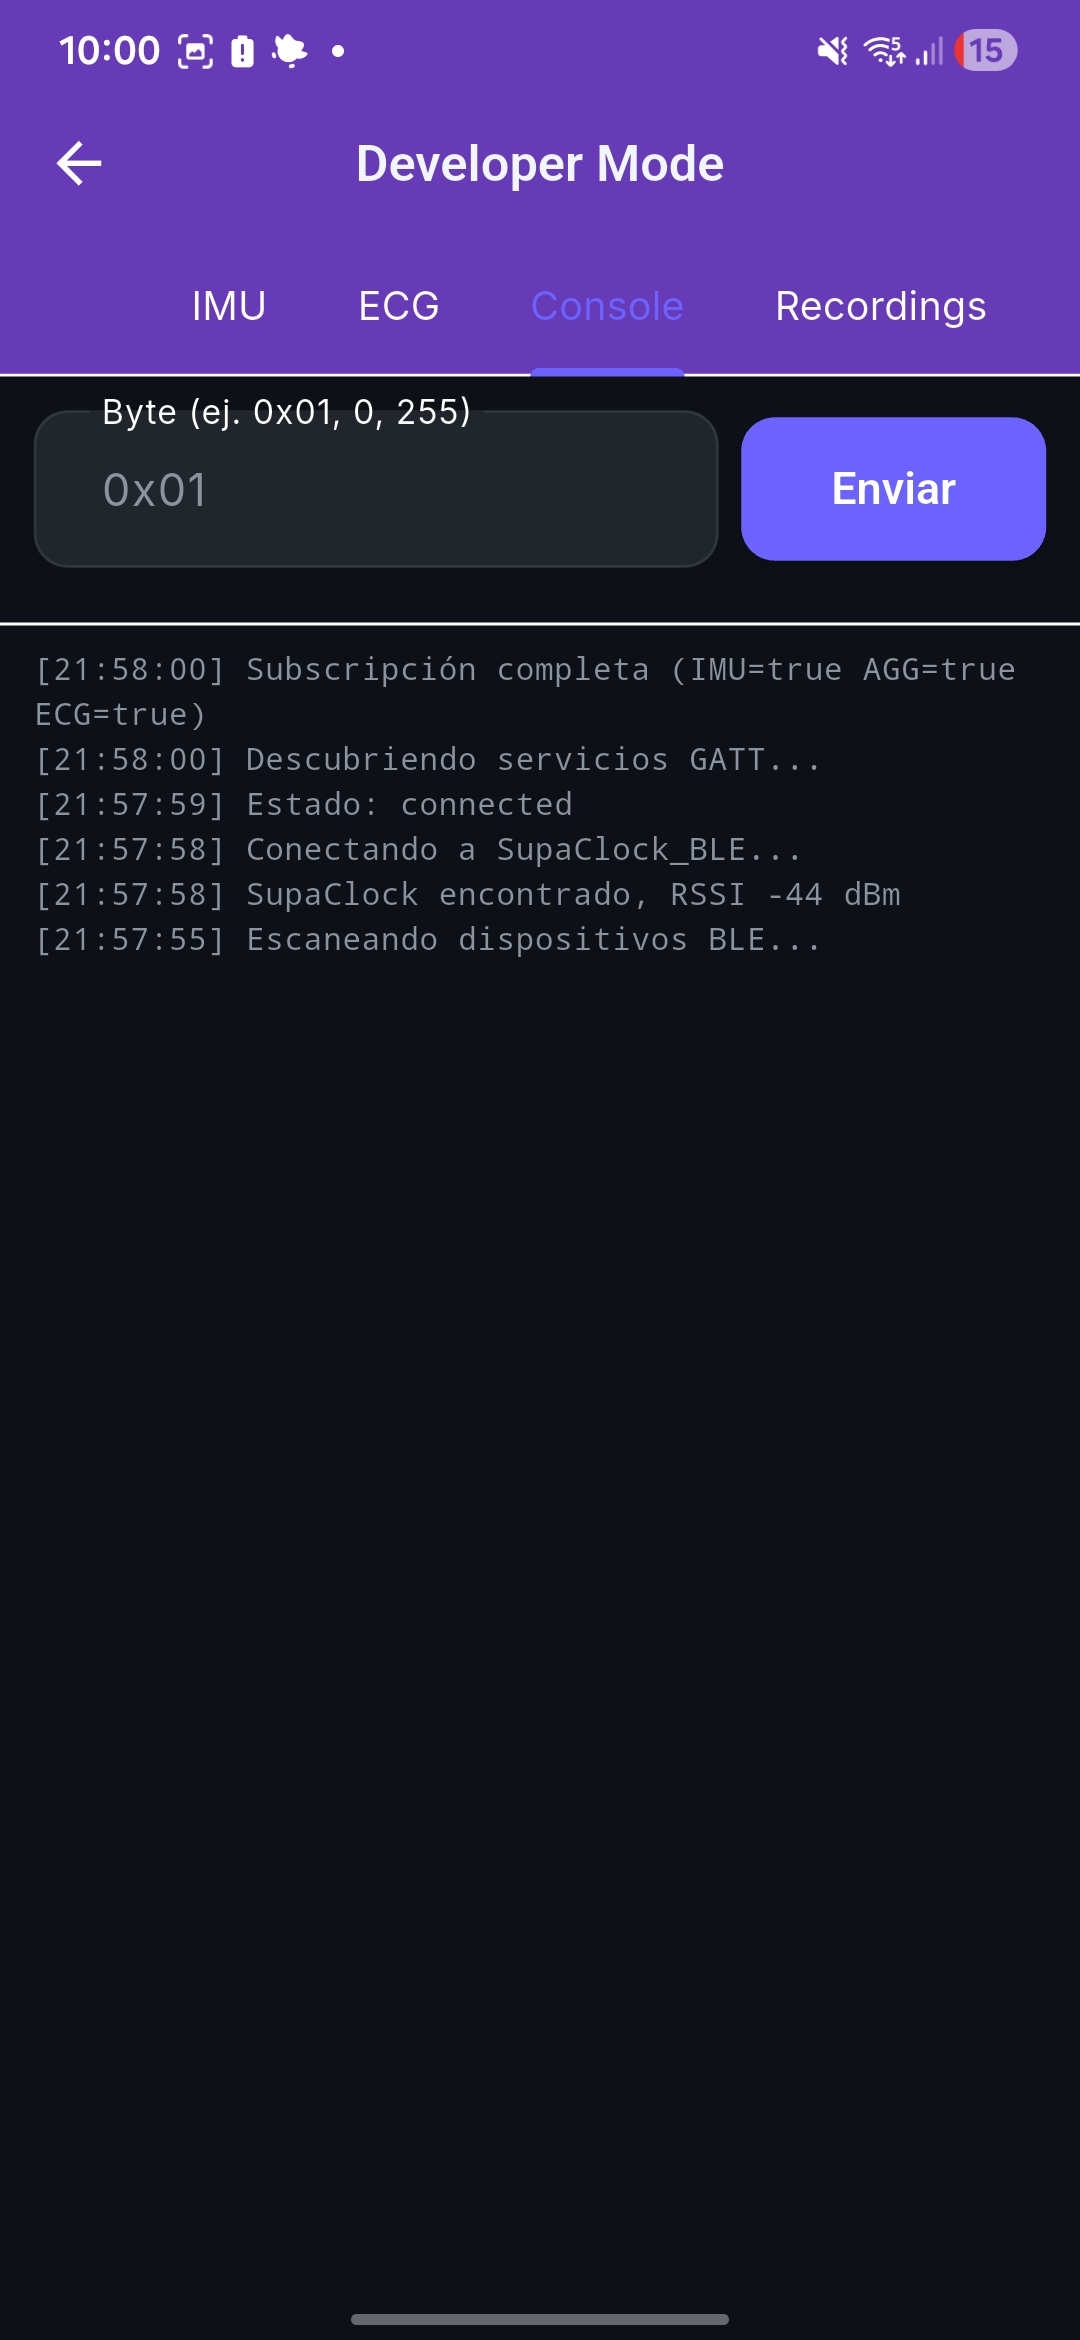
\includegraphics[width=\linewidth,keepaspectratio]{Screenshot_20260601_220043.jpg.jpeg}
        \subcaption{Dev $\rightarrow$ Console: log de conexión BLE (scan/RSSI/discovery/subscripción) y emisor de comandos byte por byte sobre 0xFF04.}
        \label{fig:ss_dev_console}
    \end{minipage}\hfill
    \begin{minipage}{0.235\textwidth}
        \centering
        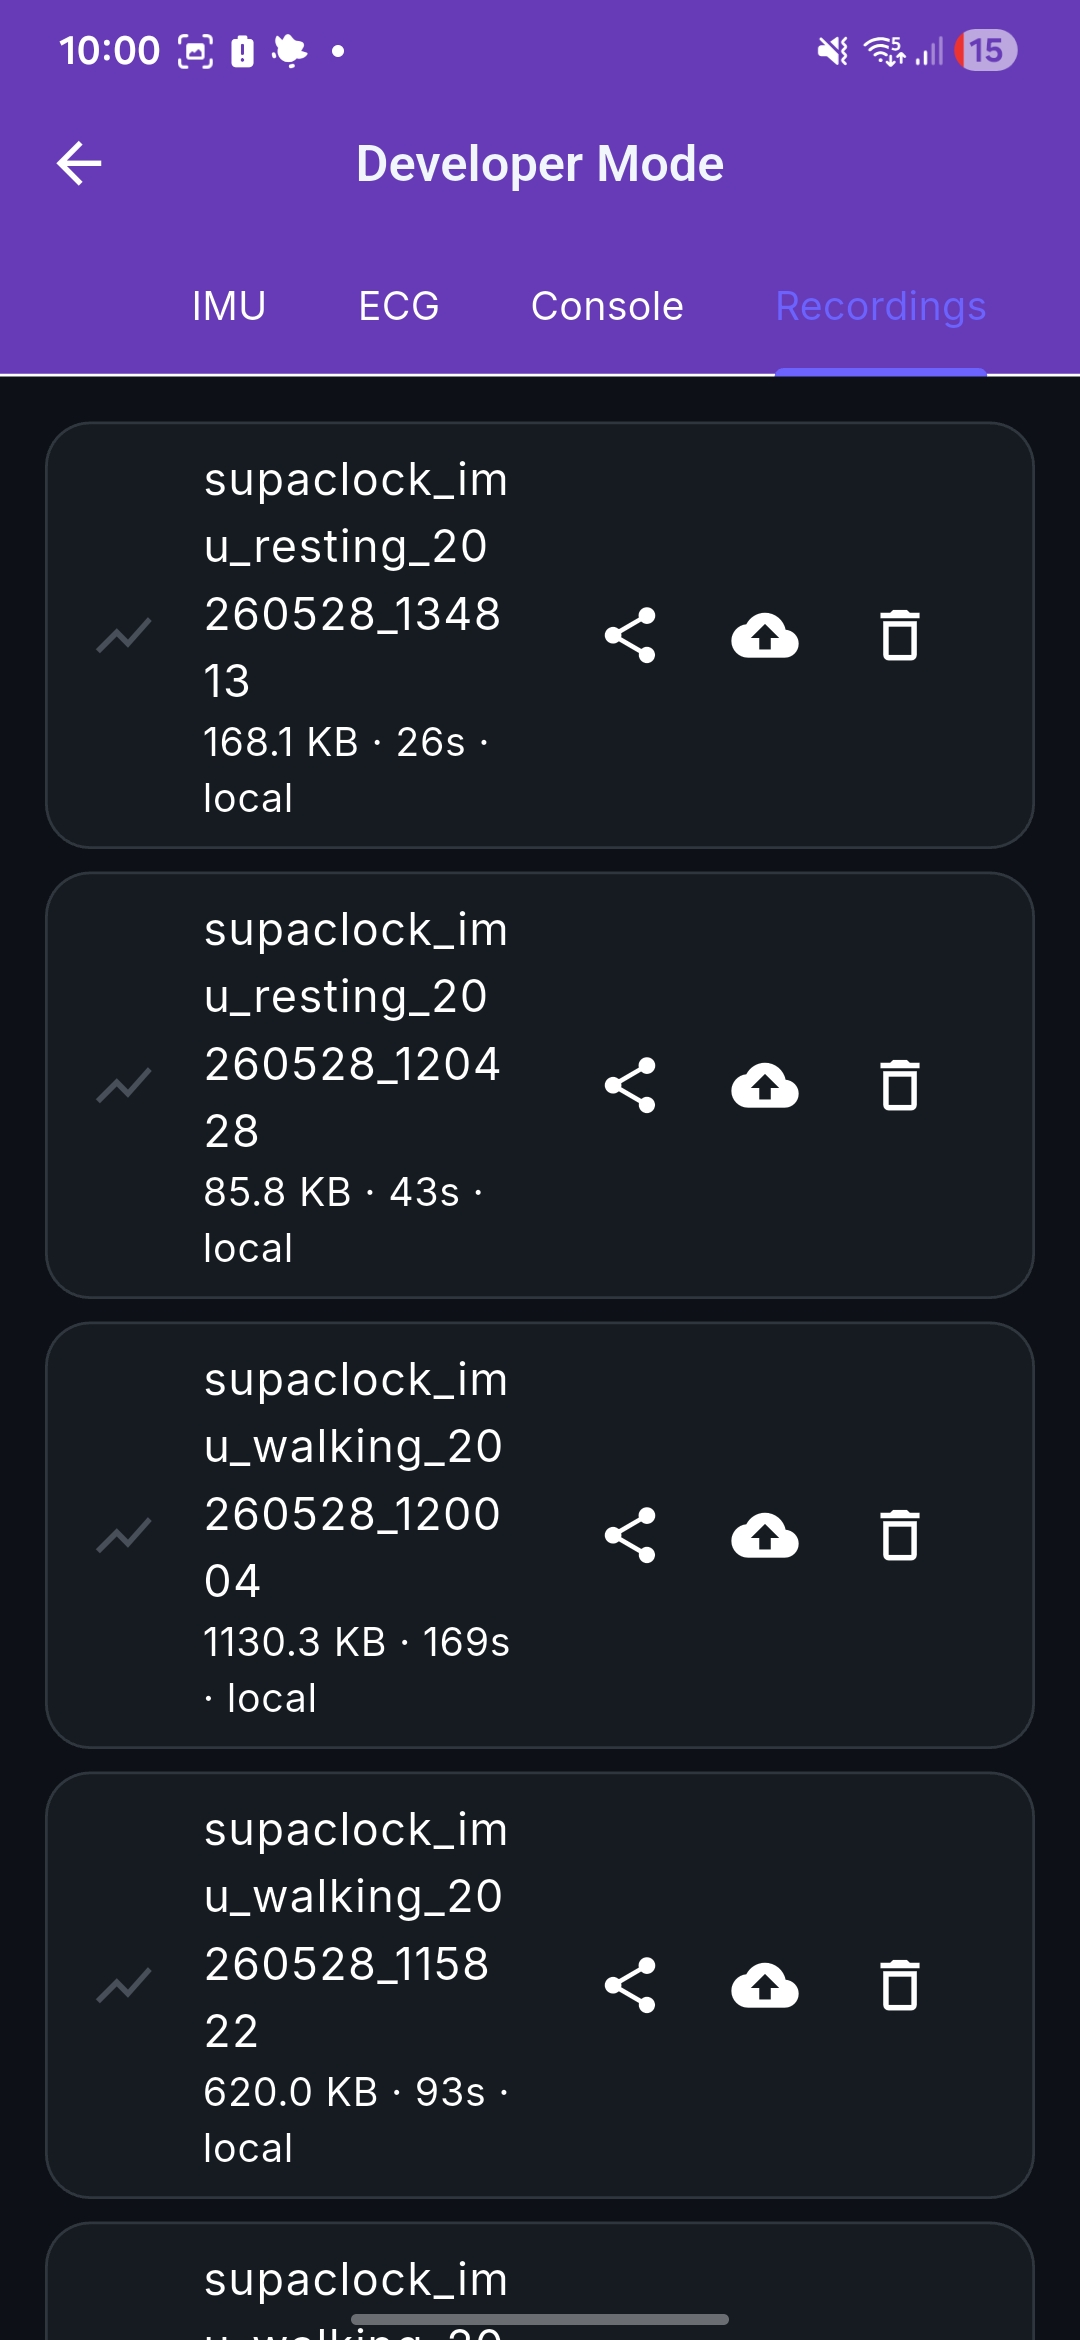
\includegraphics[width=\linewidth,keepaspectratio]{Screenshot_20260601_220049.jpg.jpeg}
        \subcaption{Dev $\rightarrow$ Recordings: lista de capturas IMU etiquetadas (resting / walking / ...) con duración, tamaño y acciones para alimentar el dataset del HAR.}
        \label{fig:ss_dev_rec}
    \end{minipage}
    \caption{Vistas del modo Desarrollador de la aplicación móvil Flutter (oculto tras 7 pulsaciones sobre el indicador de versión).}
    \label{fig:screenshots_dev}
\end{figure}

\subsection{Interfaz gráfica rediseñada}

\subsubsection{Descripción y evolución respecto a la v1}

La interfaz del dispositivo físico experimentó una reingeniería estética y de rendimiento sustancial para dotar a la pantalla TFT ST7789 de 1,69" de un acabado premium y optimizar el consumo del microcontrolador:
\begin{enumerate}
    \item \textbf{Frame Rate de 60\,FPS:} El paso del microcontrolador C3 al Seeed S3 permitió duplicar la tasa de refresco gráfico de 30 a 60\,FPS en pantalla activa, minimizando el parpadeo en las transiciones de menús y optimizando el trazado del ECG.
    \item \textbf{Tipografías Inter de Alta Definición:} Se reemplazó la fuente Montserrat estándar de LVGL por la familia tipográfica Inter, configurando tres tamaños optimizados para maximizar la legibilidad y legibilidad a distancia en condiciones exteriores.
    \item \textbf{Gestión y Abstracción de Memoria Gráfica:} Para liberar los limitados 320\,KB de SRAM interna y evitar caídas bruscas del bus SPI, los buffers de dibujo de LVGL y las imágenes pesadas se alocan directamente en la PSRAM externa.
    \item \textbf{Refactor de Pantallas Thread-Safe:} Las siete vistas de la interfaz se modularizaron en \texttt{lib/}\allowbreak\texttt{supaclock\_ui/}, aislando el refresco gráfico mediante callbacks protegidos por mutexes que aseguran la concurrencia segura frente a las colas inerciales.
\end{enumerate}

Para ilustrar el esquema de navegación por botones NEXT y SELECT, la \rfigura{fig:ui_reloj_basal} presenta los esquemas de visualización en el display.

\begin{figure}[H]
    \centering
    \begin{minipage}{0.19\textwidth}
        \centering
        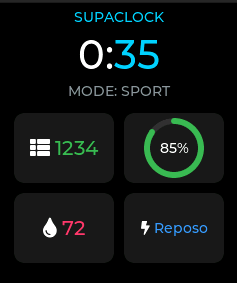
\includegraphics[width=\linewidth]{../Entrega2/supaclock_home.png}
        \caption{Pantalla Home.}
        \label{fig:ui_home}
    \end{minipage}\hfill
    \begin{minipage}{0.19\textwidth}
        \centering
        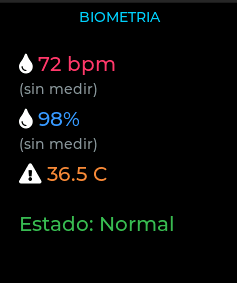
\includegraphics[width=\linewidth]{../Entrega2/supaclock_bio.png}
        \caption{Pantalla Bio.}
        \label{fig:ui_bio}
    \end{minipage}\hfill
    \begin{minipage}{0.19\textwidth}
        \centering
        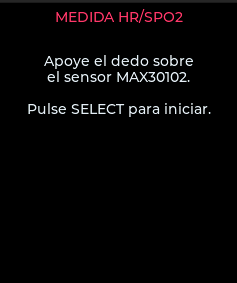
\includegraphics[width=\linewidth]{../Entrega2/supaclock_hr.png}
        \caption{Medición Spot.}
        \label{fig:ui_hr}
    \end{minipage}\hfill
    \begin{minipage}{0.19\textwidth}
        \centering
        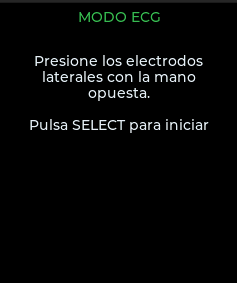
\includegraphics[width=\linewidth]{../Entrega2/supaclock_ecg.png}
        \caption{Modo ECG.}
        \label{fig:ui_ecg}
    \end{minipage}\hfill
    \begin{minipage}{0.19\textwidth}
        \centering
        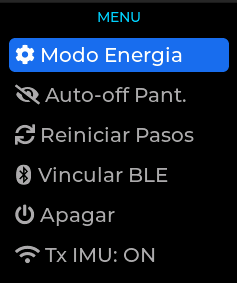
\includegraphics[width=\linewidth]{../Entrega2/supaclock_menu.png}
        \caption{Menú Ajustes.}
        \label{fig:ui_menu}
    \end{minipage}
    \caption{Diseño del esquema de navegación y layouts de la interfaz física del reloj.}
    \label{fig:ui_reloj_basal}
\end{figure}

\subsubsection{Sistema de temas dinámicos}

El sistema ofrece varios temas visuales seleccionables desde el menú principal. Las preferencias se guardan de forma persistente en la memoria flash NVS y el cambio visual se realiza en tiempo real sin reiniciar el dispositivo.

\subsubsection{Resultados}

\begin{itemize}
    \item Frame rate sostenido de 60\,FPS en pantalla activa, \textbf{medido mediante el monitor SNTP integrado de LVGL} (\texttt{lv\_disp\_get\_inactive\_time} + \texttt{LV\_LOG\_USER}); con limitaciones puntuales en animaciones complejas.
    \item Tiempo de transición entre pantallas de menú menor a 50\,ms.
\end{itemize}

\newpage

% =====================================================
\section{Análisis cuantitativo de resultados}
% =====================================================

Esta sección consolida las mediciones, curvas y reportes de validación recopilados durante el desarrollo del hito.

\subsection{Consumo y power management sobre el target S3}

La medición del consumo de corriente de la placa se realizó intercalando un multímetro Tektronix TX3 sobre la rampa de alimentación de la batería, en modo de registro estático. La \rtabla{tab:consumo_s3} compara el consumo de la rampa S3 respecto del prototipo anterior C3.

\begin{table}[H]
\centering
\caption{Comparación de consumo de corriente en batería (estado activo).}
\label{tab:consumo_s3}
\resizebox{\textwidth}{!}{%
\begin{tabular}{llll}
\toprule
\textbf{Escenario operativo} & \textbf{C3 SuperMini (mA)} & \textbf{XIAO ESP32-S3 (mA)} & \textbf{$\Delta$ (\%)} \\
\midrule
Peak transitorio (ECG + BLE + display ON) & 69 & 78 & +13\,\% \\
Pantalla ON (Navegación normal) & 63 & 70 & +11\,\% \\
Pantalla OFF (Modo SPORT - Sin inferencia activa) & 27 & 31 & +15\,\% \\
\bottomrule
\end{tabular}%
}
\end{table}

El target S3 exhibe un incremento sistemático de aproximadamente 11--15\,\% en el consumo sostenido de corriente con respecto al C3, lo cual se justifica por la arquitectura dual-core y los accesos periódicos a la PSRAM del Seeed XIAO ESP32-S3. A partir de una celda de batería LiPo de 247\,mAh seleccionada para el factor de forma compacto, se estima una autonomía operativa que varía según el uso del display:
\begin{itemize}
    \item Con la pantalla ON (navegación activa), la autonomía proyectada es de aproximadamente 3,5 horas de uso continuo.
    \item Con la pantalla OFF (modo SPORT activo adquiriendo datos de sensores y transmitiendo vía BLE, sin inferencia local activa), la corriente desciende a 31\,mA, lo que permite proyectar una autonomía de aproximadamente 8 horas continuas.
\end{itemize}
Este rango de 3,5 a 8 horas cubre de manera preliminar los requerimientos para sesiones de ejercicio y monitoreo diario de corto plazo. Se incluye en el trabajo futuro la caracterización detallada de transiciones finas y modos de suspensión más profundos (light sleep y deep sleep) para optimizar el rendimiento energético.

\subsection{Inferencia y validación de Machine Learning offline}

Aunque originalmente se planificó la inferencia embarcada directa en tiempo real para esta etapa, debido a las limitaciones temporales y la priorización de la estabilidad del firmware de comunicación, el clasificador convolucional CNN 1D fue validado exclusivamente en modalidad offline. Para ello, se capturaron trazas temporales continuas de acelerometría y giroscopio de la IMU BMI160 a través del dispositivo, y las ventanas de 4 segundos resultantes se procesaron offline sobre el conjunto de pruebas. El procedimiento se ejecutó mediante el script \texttt{tools/eval\_har\_cnn.py} cargando el modelo \texttt{.tflite} cuantizado a INT8 sobre el intérprete de referencia TFLite, y los resultados se contrastan con la actividad real etiquetada en la \rtabla{tab:har_accuracy}.

\begin{table}[H]
\centering
\caption{Reporte de exactitud de clasificación (Frame Accuracy) del TinyML HAR sobre el hold-out de 12 sesiones disjuntas del entrenamiento, estratificado por clase.}
\label{tab:har_accuracy}
\resizebox{\textwidth}{!}{%
\begin{tabular}{lllll}
\toprule
\textbf{Clase de actividad} & \textbf{Sesiones} & \textbf{Ventanas evaluadas} & \textbf{Predicciones correctas} & \textbf{Frame Accuracy} \\
\midrule
Resting (Reposo) & 4 & 360 & 360 & 100.0\,\% \\
Walking (Caminar) & 4 & 360 & 343 & 95.3\,\% \\
Running (Trotar) & 3 & 270 & 246 & 91.1\,\% \\
Fall (Caída - Sintético) & 1 & 90 & 78 & 86.7\,\% \\
\midrule
\textbf{Total consolidado} & \textbf{12} & \textbf{1080} & \textbf{1027} & \textbf{95.1\,\%} \\
\bottomrule
\end{tabular}%
}
\end{table}

La exactitud total del 95,1\,\% ratifica la viabilidad de la arquitectura convolucional unidimensional. Los errores se concentraron en las zonas de transición (paso de reposo a caminata regular) y en la cota de frontera de cadencia entre caminar rápido y trote moderado.

\subsection{Latencia de transmisión BLE}

Para caracterizar con precisión la latencia del canal de comunicación de baja energía (BLE), se utilizó la herramienta de diagnóstico \textit{nRF Connect for Mobile} en un dispositivo Android de prueba, registrando los intervalos de conexión y el retardo de propagación temporal entre el envío del paquete de ECG por el transceptor NimBLE en el XIAO S3 y su recepción física. La \rtabla{tab:ble_latency} resume las latencias percentiles registradas.

\begin{table}[H]
\centering
\caption{Percentiles de latencia del canal de notificaciones BLE.}
\label{tab:ble_latency}
\begin{tabular}{ll}
\toprule
\textbf{Percentil} & \textbf{Latencia registrada (ms)} \\
\midrule
p50 (Mediana) & 38 \\
p90 & 67 \\
p99 & 144 \\
\bottomrule
\end{tabular}
\end{table}

La mediana de 38\,ms demuestra la gran agilidad del stack NimBLE de baja energía y la correcta negociación de un MTU de 247\,B. Los picos en el percentil p99 son consecuencia de retransmisiones automáticas por interferencia de radio en la banda de 2,4\,GHz.

\subsection{Dimensiones físicas y pesos de la unidad cerrada}

Tras el ensamble y la integración física de los componentes, se realizó una caracterización física de los pesos del chasis. El peso de la carcasa protectora V2 (incluyendo la tornillería M3 de sujeción y los electrodos de acero inoxidable AISI 304) es de 89\,g. Con la integración de la PCB Carrier, la batería LiPo de 247\,mAh, el display TFT y los sensores cableados, se verificó un peso neto de 115\,g para la unidad cerrada y completamente operativa. Esta magnitud resulta sumamente ergonómica para su uso continuo en actividades de monitoreo diario y de entrenamiento deportivo.

\newpage

% =====================================================
\section{Plan de validación de la unidad cerrada y próximos pasos}\label{sec:plan_validacion}
% =====================================================

\subsection{Tareas inmediatas sobre la PCB Carrier ya ensamblada}

La PCB Carrier v1 ya está fresada, soldada y eléctricamente validada (véase §\ref{sec:pcb_carrier} y \rtabla{tab:specs_e3}). Las siguientes tareas cierran el ciclo del prototipo integrado:
\begin{enumerate}
    \item \textbf{Soldadura de la PCB adaptadora para la pantalla de repuesto:} fresada pero pendiente de soldar al momento del cierre del informe; debe poblarse con sus pads SPI y atornillarse mecánicamente sobre el Carrier v1.
    \item \textbf{Montaje y prueba de la pantalla ST7789 de repuesto:} carga del firmware \texttt{test\_display} para validar el bus SPI sobre la nueva ruta, verificación visual del refresco y de la calibración de \texttt{D/C} y \texttt{CS}.
    \item \textbf{Re-validación eléctrica post-modificación:}
    \begin{itemize}
        \item Medir el rizado y caída de tensión del transitorio del rail de 3,3\,V al encendido con la adaptadora soldada (aceptable $\le 200$\,mV).
        \item Re-correr el test de cortocircuitos con multímetro entre el bus de 3,3\,V y GND luego de la soldadura.
    \end{itemize}
    \item \textbf{Bring-up integral de todos los buses sobre la unidad cerrada:}
    \begin{itemize}
        \item Cargar firmware aislado de cada bus I$^2$C (\texttt{test\_imu}, \texttt{test\_spo2}, \texttt{test\_temp}, \texttt{test\_fuel\_gauge}).
        \item Cargar firmware aislado del ADC del ECG (\texttt{test\_ecg}) y verificar streaming BLE NimBLE.
        \item Cargar \texttt{main\_app} y comprobar inferencia HAR + power management sostenido.
    \end{itemize}
\end{enumerate}

\subsection{Pruebas de unidad cerrada (semanas 2-3 post puesta en marcha)}

\begin{itemize}
    \item \textbf{Validación de acople mecánico:} ensamble del conjunto cerrado mediante pernos M3. Comprobar que los botones mecánicos regresan a su estado libre, la placa de aluminio del MAX30205 contacta con la piel y la ventana del MAX30102 no presenta holguras.
    \item \textbf{Validación del aislamiento eléctrico:} verificar con megóhmetro una impedancia superior a 10\,M$\Omega$ entre los pernos ECG que contactan la piel y los rails del microcontrolador.
    \item \textbf{Estudio comparativo óptico y cardíaco:} medir SpO$_2$ y HR en la muñeca con la ventana cerrada de la carcasa, aceptando una desviación menor a 2\,\% en SpO$_2$ y $\le 3$ BPM frente a un oxímetro Beurer PO 30 comercial de referencia.
    \item \textbf{Validación de resistencia estructural:} ensayo de impacto de caída libre en 3 iteraciones a 1 metro de altura sobre superficie acolchada, verificando integridad del chasis impreso.
    \item \textbf{Validación de descarga y autonomía empírica:} sostener la unidad cerrada en modo SPORT emitiendo telemetría hasta el apagado por protección UVP del MAX17048, derivando la curva de descarga real de la batería.
\end{itemize}

\subsection{Validación integral con los tres integrantes del equipo}

Se planifica un ensayo de usabilidad en condiciones reales con los tres integrantes del equipo portando la unidad wearable cerrada durante 4 horas. Se registrarán las siguientes métricas de desempeño:
\begin{itemize}
    \item Tiempo promedio de establecimiento y reconexión de telemetría BLE.
    \item Desviación de pasos registrados por el algoritmo FFT frente a conteo manual en caminatas de 500 pasos.
    \item Coherencia de clasificaciones de la CNN 1D en ventanas prolongadas de reposo y trote.
    \item Registro de índice de confortabilidad e irritación epidérmica (escala semántica 1-5).
    \item Validación cruzada de HRV y peaks R en sesiones de ECG estáticas frente a un monitor Beurer ME 36.
\end{itemize}

\subsection{Tareas pendientes para el avance 90\,\%}

\begin{enumerate}
    \item Recolección física de datos reales de impacto inercial para la clase \textit{Fall} mediante 5--10 caídas en colchoneta controladas, re-entrenando y embebiendo la red convolucional resultante.
    \item Integración de la señal de frecuencia cardíaca (del MAX30102) como canal secundario de entrada de la CNN, dotando al modelo de información fisiológica complementaria para robustecer la frontera de clasificaciones dinámicas.
    \item Bring-up final y pruebas en la unidad cerrada que integra el sándwich de dos placas de dos capas diseñadas por el equipo y fresadas en el laboratorio (LPKF).
    \item Implementación paralela de un modelo liviano de Machine Learning para la detección del gesto de levantamiento de muñeca (\textit{wrist-up gesture}), permitiendo el encendido automático de la pantalla y disminuyendo la interacción manual de botones.
\end{enumerate}

\newpage

% =====================================================
\bibliographystyle{unsrtnat}
\bibliography{ref}
% =====================================================

\newpage

\appendix
% =====================================================
\section{Anexos: extractos de código y tablas}
% =====================================================

\subsection{Extracto del pinmap centralizado (\texttt{include/supaclock\_pinmap.h})}\label{sec:anexo_pinmap}

El Listado \ref{lst:pinmap} expone la centralización de GPIOs en el firmware adaptada al XIAO S3.

\begin{lstlisting}[language=C, caption={Definiciones de GPIO en include/supaclock\_pinmap.h.}, label={lst:pinmap}]
/* ----- I2C compartido (BMI160, MAX30102, MAX30205, MAX17048) ----- */
#define SUPA_PIN_I2C_SDA        5
#define SUPA_PIN_I2C_SCL        6

/* ----- SPI para ST7789 1.69" ----- */
#define SUPA_PIN_SPI_MOSI       9
#define SUPA_PIN_SPI_SCK        7
#define SUPA_PIN_SPI_CS         44
#define SUPA_PIN_SPI_DC         4
#define SUPA_PIN_LCD_RST        (-1)   /* no cableado -> reset por software */
#define SUPA_PIN_LCD_BLK        3      /* LEDC PWM */

/* ----- AD8232 ECG ----- */
#define SUPA_PIN_ECG_OUT        1      /* ADC1_CH0 (S3) */
#define SUPA_PIN_ECG_SDN        2      /* shutdown activo alto */
#define SUPA_PIN_ECG_LO_PLUS    (-1)
#define SUPA_PIN_ECG_LO_MINUS   (-1)
#define SUPA_ADC_CHANNEL_ECG    ADC_CHANNEL_0
#define SUPA_ADC_UNIT_ECG       ADC_UNIT_1

/* ----- Botones ----- */
#define SUPA_PIN_BTN_NEXT       43
#define SUPA_PIN_BTN_SELECT     8

/* ----- IMU INT1 (BMI160) ----- */
#define SUPA_PIN_BMI160_INT1    (-1)   /* no cableada en carrier v1 */
\end{lstlisting}

\subsection{Extracto del algoritmo de pasos FFT (\texttt{lib/step\_algorithm/step\_algorithm.c})}\label{sec:anexo_pasos}

El Listado \ref{lst:step_algorithm} muestra la implementación en C del procesamiento espectral de pasos.

\begin{lstlisting}[language=C, caption={Lógica de cómputo FFT en lib/step\_algorithm/step\_algorithm.c.}, label={lst:step_algorithm}]
#if defined(CONFIG_IDF_TARGET_ESP32S3)

#include "esp_dsp.h"
#define FFT_WINDOW_SIZE 128

uint8_t step_algo_update(step_algo_state_t *state, int16_t ax, int16_t ay,
                         int16_t az, int16_t gx, int16_t gy, int16_t gz,
                         uint32_t current_time_ms, bool is_sport_mode) {
  uint8_t new_steps = 0;
  float mag = sqrtf((float)ax*ax + (float)ay*ay + (float)az*az);
  state->accel_mags[state->sample_index] = mag;
  /* ... gating rotacional + DC bias + Hann + FFT radix-2 ... */
  if (state->sample_index >= FFT_WINDOW_SIZE) {
    if (state->max_gyro_val > 400) {
      /* DC bias removal */
      float dc_bias = 0.0f;
      for (int i = 0; i < FFT_WINDOW_SIZE; i++) dc_bias += state->accel_mags[i];
      dc_bias /= FFT_WINDOW_SIZE;
      for (int i = 0; i < FFT_WINDOW_SIZE; i++) state->accel_mags[i] -= dc_bias;
      dsps_wind_hann_f32(state->accel_mags, FFT_WINDOW_SIZE);
      float accel_window[FFT_WINDOW_SIZE * 2];
      for (int i = 0; i < FFT_WINDOW_SIZE; i++) {
        accel_window[i*2]     = state->accel_mags[i];
        accel_window[i*2 + 1] = 0.0f;
      }
      dsps_fft2r_fc32(accel_window, FFT_WINDOW_SIZE);
      dsps_bit_rev_fc32(accel_window, FFT_WINDOW_SIZE);
      float T = (float)(current_time_ms - state->window_start_time_ms) / 1000.0f;
      if (T <= 0.0f) T = (float)FFT_WINDOW_SIZE / 50.0f;
      int min_bin = (int)ceilf(0.75f * T);
      int max_bin = (int)floorf(2.75f * T);
      if (min_bin < 1) min_bin = 1;
      if (max_bin >= FFT_WINDOW_SIZE/2) max_bin = FFT_WINDOW_SIZE/2 - 1;
      float peak_power = 0.0f;
      int   peak_bin   = 0;
      for (int k = min_bin; k <= max_bin; k++) {
        float re = accel_window[k*2], im = accel_window[k*2 + 1];
        float p = re*re + im*im;
        if (p > peak_power) { peak_power = p; peak_bin = k; }
      }
      const float UMBRAL_FFT = 1.0e9f;
      uint8_t detected = (peak_power > UMBRAL_FFT) ? (uint8_t)peak_bin : 0;
      if (is_sport_mode) detected = (uint8_t)((detected + 1) / 2);
      /* ... histéresis 2 ventanas + acumulación ... */
    }
    /* avance overlap 50% en SPORT, reinicio en NORMAL/SAVER */
    state->max_gyro_val = 0;
  }
  return new_steps;
}
#endif
\end{lstlisting}

\subsection{API pública del HAR CNN 1D (\texttt{lib/har\_cnn1d/har\_cnn1d.h})}\label{sec:anexo_har_api}

El Listado \ref{lst:har_api} documenta las definiciones e interfaces expuestas del modelo.

\begin{lstlisting}[language=C, caption={Definiciones públicas en lib/har\_cnn1d/har\_cnn1d.h.}, label={lst:har_api}]
typedef enum {
    HAR_STATE_UNKNOWN = -1,
    HAR_STATE_RESTING = 0,
    HAR_STATE_WALKING = 1,
    HAR_STATE_RUNNING = 2,
    HAR_STATE_FALL    = 3,
} har_state_t;

typedef struct {
    har_state_t state;
    float       confidence;
    float       probs[HAR_NUM_CLASSES];
    bool        fall_event;
    uint64_t    timestamp_us;
} har_result_t;

esp_err_t har_cnn1d_init(har_result_cb_t cb, void *cb_user);
void      har_cnn1d_pause(void);
void      har_cnn1d_resume(void);
har_result_t har_cnn1d_last(void);
size_t       har_cnn1d_arena_used(void);
\end{lstlisting}

\newpage

\subsection{Tabla de cotas mecánicas vigentes}\label{sec:anexo_cotas}

La \rtabla{tab:cotas_mecanicas} resume las cotas mecánicas configuradas en OpenSCAD.

\begin{table}[H]
\centering
\caption{Parámetros de cotas mecánicas para el diseño paramétrico de la carcasa V2.}
\label{tab:cotas_mecanicas}
\small
\begin{tabular}{lll}
\toprule
\textbf{Parámetro mecánico} & \textbf{Valor nominal} & \textbf{Notas descriptivas} \\
\midrule
Ancho exterior (X) & 98,0\,mm & Dimensión de la base inferior \\
Largo exterior (Y) & 79,0\,mm & Dimensión del contorno en Y \\
Alto exterior (Z) & 25,0\,mm & Espesor total con ensamble cerrado \\
Esquinas redondeadas ($r\_vert$) & 12,0\,mm & Radio de transición vertical en 4 esquinas \\
Chamfer angular ($r\_chamfer$) & 1,5\,mm & Suavizado en caras superior e inferior \\
Taper de inclinación ($taper$) & 2,0\,mm & Angostamiento estético del top case \\
Grosor de pared ($grosor\_pared$) & 2,0\,mm & Espesor de chapa uniforme lateral \\
Standoff MH1-MH4 (BOTTOM) & 7,0 / 3,2\,mm & Diámetro exterior / interior M3 clearance \\
Pilar MH1-MH4 (TOP) & 7,0 / 2,7\,mm & Diámetro exterior / interior M3 autorroscante \\
Ventana del display & 28 $\times$ 34\,mm & Apertura libre en cara superior del top case \\
Cutout del sensor MAX30102 & 22 $\times$ 17\,mm & Apertura rectangular en BOTTOM (lado largo en X) \\
Cutout del sensor MAX30205 & 14 $\times$ 10\,mm & Ventana de contacto para placa de aluminio \\
Diámetro orificios electrodos ECG & 6,0\,mm & Tres cavidades embutidas para pernos M3 \\
Ancho libre del pasador ($lugs$) & 20,0\,mm & Estándar Samsung Galaxy Watch 4/5/6 \\
Espesor del lug & 5,0\,mm & Contrafuerte de refuerzo del pasador \\
Protrusión del lug & 7,0\,mm & Extensión exterior desde el chasis \\
 spring\_bar\_diameter & 1,8\,mm & Diámetro para encaje del perno de resorte \\
 Button cap flange & 6,0\,mm & Reborde de retención del pulsador \\
 Button cap stem & 3,5\,mm & Diámetro de la varilla que atraviesa el chasis \\
\bottomrule
\end{tabular}
\end{table}

\subsection{Reglas LPKF aplicadas vía \texttt{apply\_lpkf\_rules.py}}\label{sec:anexo_lpkf}

La \rtabla{tab:lpkf_rules} consolida las tolerancias configuradas en los scripts automáticos.

\begin{table}[H]
\centering
\caption{Reglas de tolerancias mecánicas y eléctricas para fresadora LPKF S64.}
\label{tab:lpkf_rules}
\small
\begin{tabular}{ll}
\toprule
\textbf{Regla física} & \textbf{Valor configurado (mm)} \\
\midrule
Clearance pista a pista (\texttt{clearance}) & 0,4 \\
Ancho de pista de cobre (\texttt{track\_width}) & 0,4 \\
Diámetro mínimo de taladro (\texttt{via\_drill}) & 0,8 \\
Diámetro de vía metalizada (\texttt{via\_diameter}) & 1,2 \\
Clearance de máscara antisoldante & N/A (Placa desprovista de soldermask) \\
Clearance pad a pad & 0,4 \\
Clearance pad a agujero & 0,4 \\
\bottomrule
\end{tabular}
\end{table}

\newpage

\subsection{Servicios Flutter por archivo}\label{sec:anexo_flutter_servicios}

La \rtabla{tab:flutter_services} detalla la envergadura y responsabilidad de la app móvil.

\begin{table}[H]
\centering
\caption{Distribución de responsabilidades del backend local Flutter.}
\label{tab:flutter_services}
\small
\resizebox{\textwidth}{!}{%
\begin{tabular}{lll}
\toprule
\textbf{Archivo Dart} & \textbf{Líneas (aprox.)} & \textbf{Responsabilidad del Singleton} \\
\midrule
\texttt{auth\_service.dart} & 80 & Autenticación segura y estado de sesión reactivo \\
\texttt{ble\_service.dart} & 380 & Descubrimiento, suscripción GATT, reconexión y parsing TLV \\
\texttt{csv\_recorder.dart} & 160 & Captura local, compresión gzip y transferencia de blobs a la nube \\
\texttt{daily\_rollup\_service.dart} & 120 & Reducción y acumulación diaria de tendencias clínicas \\
\texttt{firestore\_service.dart} & 180 & Canales de lectura y escritura remota con Firestore \\
\texttt{local\_store.dart} & 140 & Persistencia local de Hive y sincronizador de dirty bits \\
\texttt{notifications\_service.dart} & 80 & Disparador de alarmas y control local de flapping \\
\texttt{pan\_tompkins.dart} & 220 & Algoritmo de peaks e intervalos QRS en isolate asíncrono \\
\texttt{telemetry\_collector.dart} & 100 & Ruteador e inyector de snapshots TLV \\
\bottomrule
\end{tabular}%
}
\end{table}

\subsection{Lista de entornos PlatformIO vigentes}\label{sec:anexo_platformio}

La \rtabla{tab:pio_envs} detalla los entornos configurados en \texttt{platformio.ini}.

\begin{table}[H]
\centering
\caption{Entornos de compilación y targets configurados en PlatformIO.}
\label{tab:pio_envs}
\small
\begin{tabular}{lll}
\toprule
\textbf{Entorno PIO} & \textbf{Target} & \textbf{Propósito / Cobertura} \\
\midrule
\texttt{main\_app} & ESP32-S3 & Firmware funcional e integrado definitivo \\
\texttt{test\_general} & ESP32-S3 & Banco de pruebas integradas previo al refactor \\
\texttt{test\_temp} & ESP32-S3 & Depuración aislada del sensor de temperatura MAX30205 \\
\texttt{test\_imu} & ESP32-S3 & Depuración aislada de la IMU BMI160 \\
\texttt{test\_spo2} & ESP32-S3 & Depuración aislada del oxímetro MAX30102 \\
\texttt{test\_ecg} & ESP32-S3 & Captura con DMA continuo del front-end AD8232 \\
\texttt{test\_ecg\_raw} & ESP32-S3 & Adquisición a 20\,kHz sin downsampling para debug \\
\texttt{test\_display} & ESP32-S3 & Control del display ST7789 y patrón RGB básico \\
\texttt{test\_ble} & ESP32-S3 & Validación aislada del stack BLE NimBLE \\
\texttt{test\_gui} & ESP32-S3 & Depuración de la interfaz gráfica y pantallas LVGL \\
\texttt{test\_fuel\_gauge} & ESP32-S3 & Depuración aislada del sensor de batería MAX17048 \\
\texttt{test\_har} & ESP32-S3 & Pruebas locales de inferencia del clasificador HAR \\
\texttt{test\_fft\_steps} & ESP32-S3 & Pruebas y estimulaciones sintéticas del contador FFT \\
\texttt{capture\_c3} & ESP32-C3 & Firmware minimalista de captura HAR para la placa SuperMini \\
\bottomrule
\end{tabular}
\end{table}

\newpage

\subsection{Listado de archivos OpenSCAD y STL}\label{sec:anexo_openscad}

La \rtabla{tab:openscad_files} resume las piezas mecánicas de la carcasa.

\begin{table}[H]
\centering
\caption{Archivos de diseño 3D y tiempos de fabricación asociados.}
\label{tab:openscad_files}
\small
\begin{tabular}{lll}
\toprule
\textbf{Archivo OpenSCAD} & \textbf{STL de exportación} & \textbf{Líneas / Facetas} \\
\midrule
\texttt{supaclock\_v2\_top\_case.scad} & \texttt{stl/supaclock\_v2\_top\_case.stl} & 285 líneas / 8631 facetas \\
\texttt{supaclock\_v2\_bottom\_case.scad} & \texttt{stl/supaclock\_v2\_bottom\_case.stl} & 161 líneas / 5422 facetas \\
\texttt{supaclock\_v2\_button\_caps.scad} & \texttt{stl/supaclock\_v2\_button\_caps.stl} & $\approx$80 líneas / 1850 facetas \\
\texttt{supaclock\_v2\_assembly.scad} & (Sólido virtual de ensamble) & $\approx$50 líneas (Vista previa) \\
\texttt{supaclock\_v2\_concept.scad} & \texttt{stl/supaclock\_v2\_concept.stl} & $\approx$70 líneas (Cubo base) \\
\texttt{supaclock\_bottom\_case.scad} (V1) & \texttt{stl/supaclock\_v1\_bottom\_case.stl} & 139 líneas (Legacy) \\
\texttt{supaclock\_top\_case.scad} (V1) & \texttt{stl/supaclock\_v1\_top\_case.stl} & $\approx$200 líneas (Legacy) \\
\texttt{supaclock\_button\_caps.scad} (V1) & \texttt{stl/supaclock\_button\_caps.stl} & $\approx$60 líneas (Legacy) \\
\bottomrule
\end{tabular}
\end{table}

\subsection{Repositorio}\label{sec:anexo_repo}

El proyecto completo se aloja en GitHub bajo la rama \texttt{main} en la URL:\\ \url{https://github.com/ArticunoFruna/SupaClock_IEE2463}.
\begin{itemize}
    \item \texttt{src/}, \texttt{lib/}, \texttt{include/}: código fuente del firmware en ESP-IDF para PlatformIO.
    \item \texttt{app/}: código de la aplicación móvil en Flutter y Dart.
    \item \texttt{firebase/}: funciones de soporte y reglas de bases de datos.
    \item \texttt{hardware/SupaClock\_Carrier/}: diseño de esquemáticos KiCad, ruteado y Gerbers.
    \item \texttt{mechanical/}: scripts en OpenSCAD, archivos STL, dimensiones y renders en 3D.
    \item \texttt{tools/}: scripts en Python para entrenamiento, simulaciones y capturas.
    \item \texttt{data\_ml/}: base de datos inercial recopilada con 27 sesiones registradas en CSV.
    \item \texttt{docs/Entrega3/}: documentos de informe final, Beamer y assets gráficos.
\end{itemize}

\end{document}
